% Ltex language=en
% \documentclass[12pt, 1p, review, number]{elsarticle}
\documentclass[3p,twocolumn,preprint]{elsarticle}
%\documentclass[10pt,a4paper,3p,twocolumn]{elsarticle}
% \documentclass[5p,preprint,twocolumn]{elsarticle}
%----------------------------------------------------------------------
%                     Loading of packages
%----------------------------------------------------------------------

% for cutting words
\usepackage[utf8]{inputenc}
% a font close to that chosen by Elsevier
\usepackage[bitstream-charter]{mathdesign}
% for accentuated characters
%\usepackage[T1]{fontenc}
\geometry{top=2cm,left=1.5cm,bottom=2cm,right=1.5cm}
\usepackage{multicol}
% For treating ps:
\usepackage{psfrag}
% For subfigures
\usepackage{graphicx}
\usepackage{subcaption}
\usepackage{placeins}
% For tables
\usepackage{array}
\usepackage{multirow}
\usepackage{hhline}
\usepackage{colortbl}
\usepackage{tabulary}
\usepackage{etoolbox}
% For citations
\usepackage[numbers]{natbib}
%\biboptions{longnamesfirst,angle,semicolon}
%\citetstyle{nature}
% For color
\usepackage{color}
\usepackage{xcolor}
% For spacing
\usepackage{setspace}
%\doublespacing
\singlespacing
%\onehalfspacing
% For maths
\usepackage{amsmath, amsfonts}
\usepackage[squaren,ashgrey]{SIunits}
% For Line numbering
\usepackage[pagewise,modulo]{lineno}
%\linenumbers
% For special characters
\usepackage{pifont}
%
\usepackage[pagebackref,colorlinks=True]{hyperref}
\usepackage{wasysym}
\usepackage{color}
\usepackage{cleveref}
\crefformat{figure}{(Fig.~#2#1#3)}
\usepackage{hyperref}
\usepackage[hyperpageref]{backref}
\usepackage{lipsum}
\usepackage{booktabs} % To thicken table lines

%----------------------------------------------------------------------
%                     Commands
%----------------------------------------------------------------------
\renewcommand*{\overrightarrow}[1]{\vbox{\halign{##\cr \tiny\rightarrowfill\cr\noalign{\nointerlineskip\vskip1pt}$#1\mskip2mu$\cr}}}
%% Degree character
\DeclareTextSymbol{\degr}{T1}{6}
\newcommand{\degre}[0]{\degr C}
\DeclareUnicodeCharacter{2212}{-}
% MPam^0.5 character
\newcommand{\mpa}[0]{\mbox{MPa}\sqrt{\mbox{m}}}
%mettre de nouilles sous les tenseurs
\newcommand{\ve}[1]{{\underline{#1}}}
\def\ten#1{\oalign{$#1$\crcr\hidewidth$\scriptscriptstyle\sim$\hidewidth}} 
% derivee seconde
\newcommand{\fda}[2]{\displaystyle \frac{\partial\,{#1}}{\partial\, {#2}}}
% et al. for citations
\newcommand{\etal}[0]{{\em et al.}}
\renewcommand*\contentsname{\large{Table of contents}}
\def \hfillx {\hspace*{ -\linewidth} \hfill} % remplir espacement horizontal entre deux sous-figures de façon à remplir toute la largeur du texte.
%----------------------------------------------------------------------
%                     Colors
%----------------------------------------------------------------------
\definecolor{ashgrey}{rgb}{0.7, 0.75, 0.71}
%----------------------------------------------------------------------
%                     Pre-Document
%----------------------------------------------------------------------
\journal{Applied Energy}
%----------------------------------------------------------------------
%                     Document
%----------------------------------------------------------------------
\begin{document}

\tableofcontents

\begin{frontmatter}

%% Title, authors and addresses

%% use the tnoteref command within \title for footnotes;
%% use the tnotetext command for theassociated footnote;
%% use the fnref command within \author or \address for footnotes;
%% use the fntext command for theassociated footnote;
%% use the corref command within \author for corresponding author footnotes;
%% use the cortext command for theassociated footnote;
%% use the ead command for the email address,
%% and the form \ead[url] for the home page:
%% \title{Title\tnoteref{label1}}
%% \tnotetext[label1]{}
%% \author{Name\corref{cor1}\fnref{label2}}
%% \ead{email address}
%% \ead[url]{home page}
%% \fntext[label2]{}
%% \cortext[cor1]{}
%% \address{Address\fnref{label3}}
%% \fntext[label3]{}

\title{Ear canal dynamic motion piezoelectric energy harvester using a bistable oscillator cycled by coupled hydraulic switches made of collapsed flexible tubes.}

%% use optional labels to link authors explicitly to addresses:
%% \author[label1,label2]{}
%% \address[label1]{}
%% \address[label2]{}


\address[symme]{Laboratoire SYMME - Université Savoie Mont Blanc, 7 Chemin de Bellevue, 74940, Annecy}
\address[critias]{Laboratoire Critias - École de Technologie Supérieure, 1100 Rue Notre-Dame Ouest, Montréal, QC, H3C 1K3}


\author[symme]{Tigran AVETISSIAN}
\author[symme]{Fabien FORMOSA}
\author[symme]{Adrien BADEL}

\author[critias]{Michel DEMUYNCK}
\author[critias]{Aidin DELNAVAZ}
\author[critias]{Jérémy VOIX}


\begin{abstract}
%% Text of abstract
\end{abstract}

\begin{keyword}
%% Keywords
\end{keyword}

\end{frontmatter}

%\linenumbers

%% main text
%/!\/!\/!\/!\/!\/!\/!\/!\/!\/!\/!\/!\/!\/!\/!\/!\/!\/!\/!\/!\/!\/!\/!\/!\%
\section{INTRODUCTION}
\label{INTRODUCTION} % Ltex language=en
%/!\/!\/!\/!\/!\/!\/!\/!\/!\/!\/!\/!\/!\/!\/!\/!\/!\/!\/!\/!\/!\/!\/!\/!\%

The growing use of wireless devices and the miniaturization of electronic circuits have led to significant progress on the energy consumption of mobile devices around the human body. Energy harvesting methods have also been studied on purpose, in order to complement their power supply and enhance the autonomy of the batteries. In-ear devices such as hearing aids and cochlear implants are powered by disposable fuel cells or rechargeable batteries. The energy consumption of the best integrated devices in the literature converges around $17$J for a 10 hours daily use \cite{Scherer2019,Yip2015,Kulah2022}. Woodruff \emph{et al.} showed that patients using hearing aids sometimes struggle to change and select batteries for their devices \cite{Woodruff2021}. Another statistical study revealed that the majority of hearing aid and cochlear implants users prefer disposable batteries for the long autonomy, but would have liked rechargeable solutions if the battery cycle was sufficient to complete the day \cite{PracticesAudiology2016}. Also, the long term use makes the rechargeable solutions a more economical and more ecological choice compared to the disposable fuels. These arguments motivate the development of energy harvesting systems to enhance the autonomy of the batteries in order to prevent the premature discharge of in-ear devices.\\
The common sources are ambient such as solar or wind energy but their availability in the low size environment of the application context makes them not suitable for exploitation.
The activities of the human body generate a considerable amount of energy of different natures. Among them, the electrochemical energy from the inner ear \cite{Mercier2012}, the kinetic energy from walking or head movements \cite{Azimi2021,Smilek2016}, the body heat thermal energy \cite{Kim2014}, the strain energy from the skin deformation \cite{Jin2021} could be harvested for in-ear applications. The most relevant energy source for cochlear implants or hearing aids is the ear canal mechanical deformation as it is directly located in the area of the application. Delnavaz \emph{et al.} first showed in 2012 that the jaw movements changes de ear canal geometry during mastication. The figure \ref{fig:TMJ_on_earcanal} schematizes the mechanical interaction between the temporomandibular joint and the ear canal when the jaw is opened and when it is closed.
%%%%%%%%%%%%%%%%%%%%%%%%%%%%%%%%%%%%%%
\begin{figure}[!htbp]
	\centering
	\captionsetup{justification=centering}
	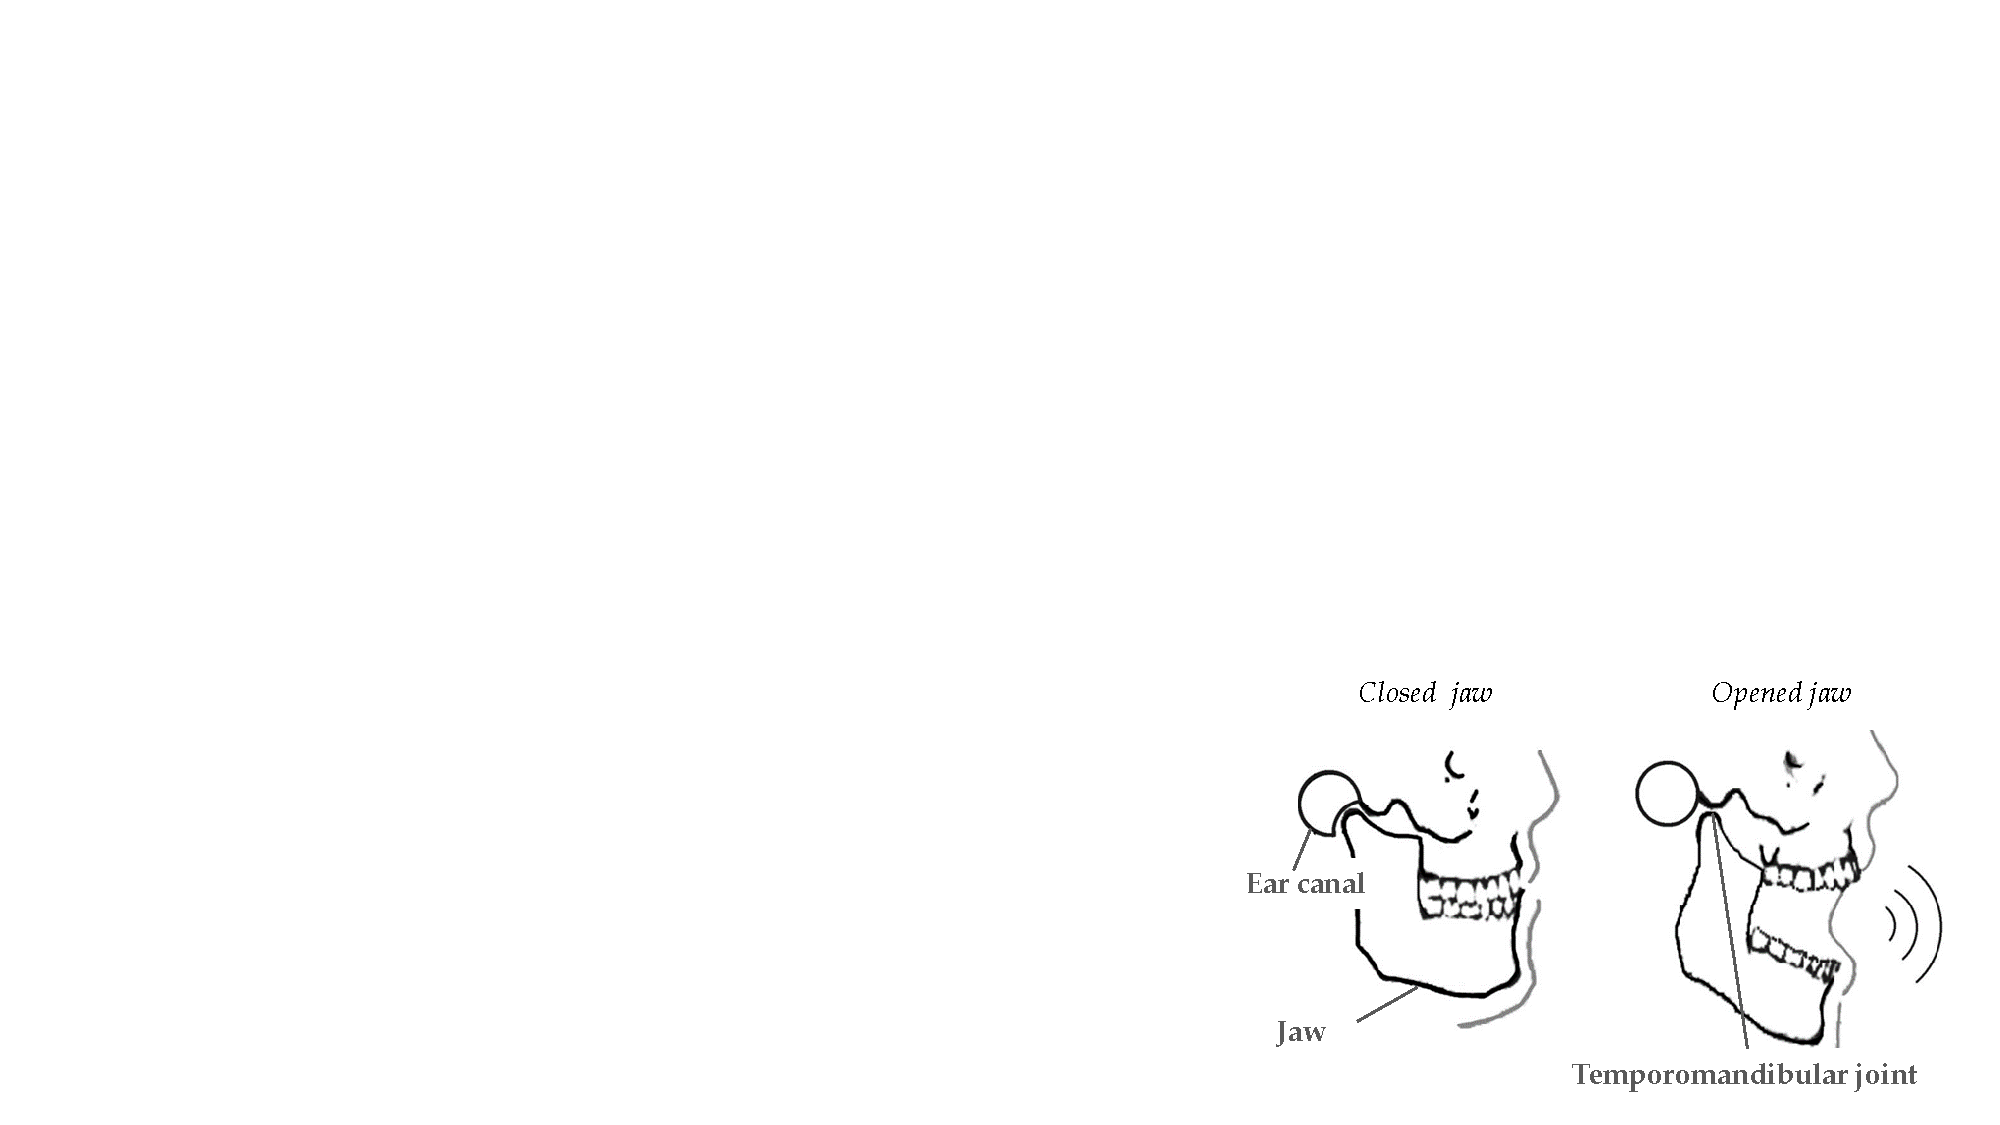
\includegraphics[trim={21cm 0cm 0cm 11.2cm},clip, width=0.9\linewidth]{figures/TMJ_on_earcanal.pdf}
	\caption{Mechanical interaction between the temporomandibular joint and the ear canal during jaw movements \cite{Delnavaz2012}}
	\label{fig:TMJ_on_earcanal}
\end{figure}
%%%%%%%%%%%%%%%%%%%%%%%%%%%%%%%%%%%%%%%
Carioli \emph{et al.} used a personalized earplug molding technic with a 3D scanner to reveal a global bending movement and a local compression area in the ear canal during mastication \cite{Carioli2016} (fig. \ref{fig:molding}). These two mechanical deformations represent an available energy source that can be exploited. This study first quantified the flexion energy amount to $5$mJ per mastication with a standard deviation of $4.9$mJ. The radial compression energy was also estimated to $1.3$mJ with $1.5$mJ of standard deviation. Besides this work, the literature exposes two technological solutions adapted to the extraction of the mechanical deformation energy in the ear canal. \\
%%%%%%%%%%%%%%%%%%%%%%%%%%%%%%%%%%%%%%
\begin{figure*}[!htbp]
	\centering
	\captionsetup{justification=centering}
	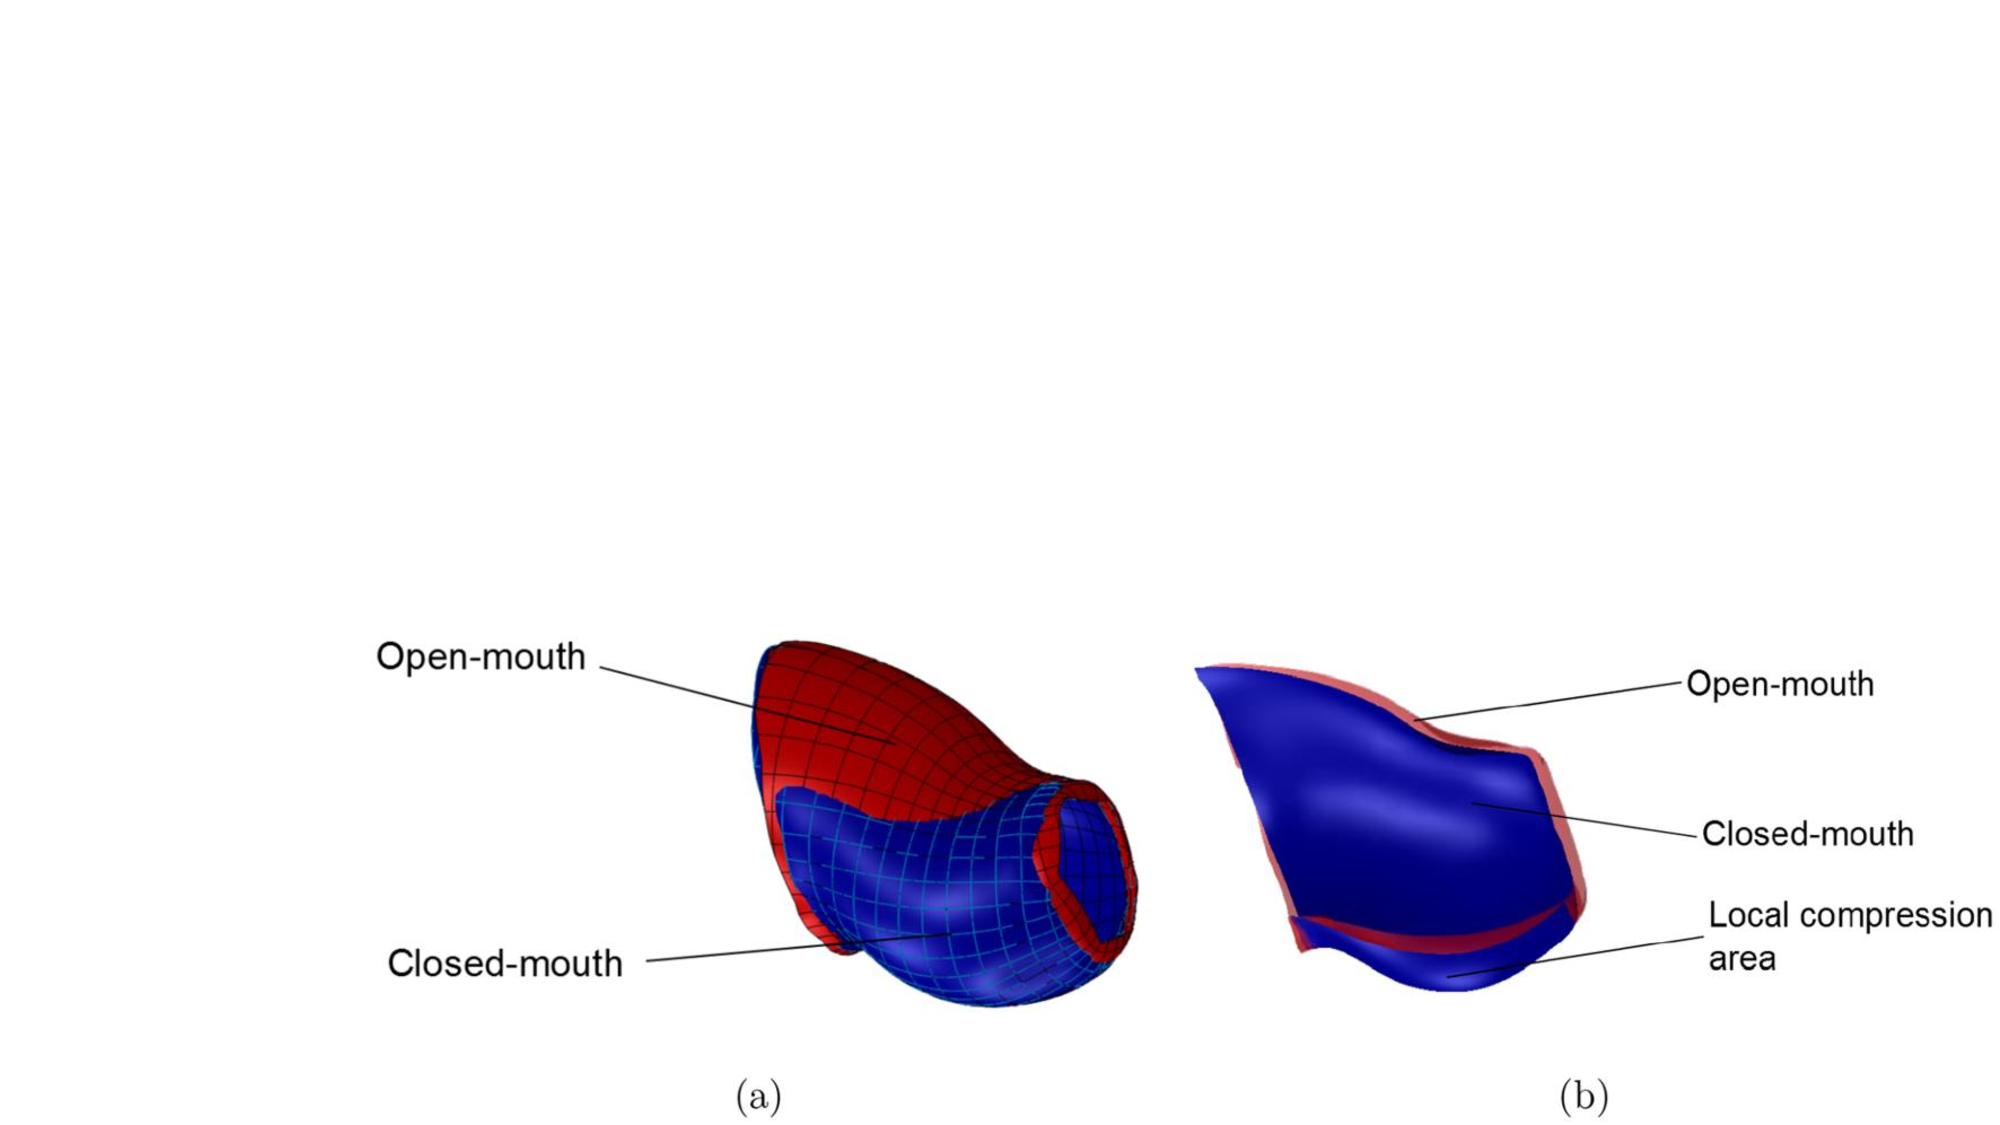
\includegraphics[trim={6cm 0cm 0cm 10cm},clip, width=0.6\linewidth]{figures/molding.pdf}
	\caption{(a) Earcanal in two extreme positions showing a global bending movement of the earcanal (b) Earcanal sectional view in two extreme positions showing a local compression area of the earcanal. \cite{Carioli2016}}
	\label{fig:molding}
\end{figure*}
%%%%%%%%%%%%%%%%%%%%%%%%%%%%%%%%%%%%%%%
Delnavaz \emph{et al.} first developed a flexible piezoelectric harvester made of a silicon earplug with a PVDF layer \cite{Delnavaz2013} (fig. \ref{fig:critias_piezo}). The earplug has been melted on the subject in order to maximize the contact surface with the ear canal. The harvester is capable of exploiting both the flexion and the compression energy sources. The experimental prototype presented on figure \ref{fig:critias_piezo} was able to extract $44$µJ from a normal mastication cycle. The soft materials facilitate the bio-integration of the harvester but the PVDF low electromechanical coupling coefficient results in an energy conversion efficiency below $1\%$. A hydroelectromagnetic energy harvester was also developed by the same researchers \cite{Delnavaz2012}. The figure \ref{fig:critias_emag} shows the harvester components and experimental test setup. The energy is extracted by a liquid filled earplug whose internal volume and pressure vary as a result of the radial compression of the ear canal internal walls during the jaw movements. These variations put into motion a moving magnet translating in a water column surrounded by a copper coil. The energy was harvested by electromagnetic induction and experimentally evaluated at 0.2µJ per mastication cycle. The hydraulic energy extraction limits the energy source to the radial compression as the ear canal global flexion does not generate any volume variation in the earplug. The low conversion efficiency ($<1\%$) is a consequence of the use of electromagnetic transduction for a low frequency energy source (1.57Hz) and a small scale application \cite{Kulah2008,Priya2017}. However, the hydraulic transmission interface allows the use of more complex and voluminous technological solutions since the energy becomes available outside the small ear canal volume. The table \ref{tab:harvesters_ear} summarizes the existing harvesters that exploit the ear canal mechanical deformation energy. \\
%%%%%%%%%%%%%%%%%%%%%%%%%%%%%%%%%%%%%%%
\begin{figure}[!htbp]
	\centering
	\captionsetup{justification=centering}
	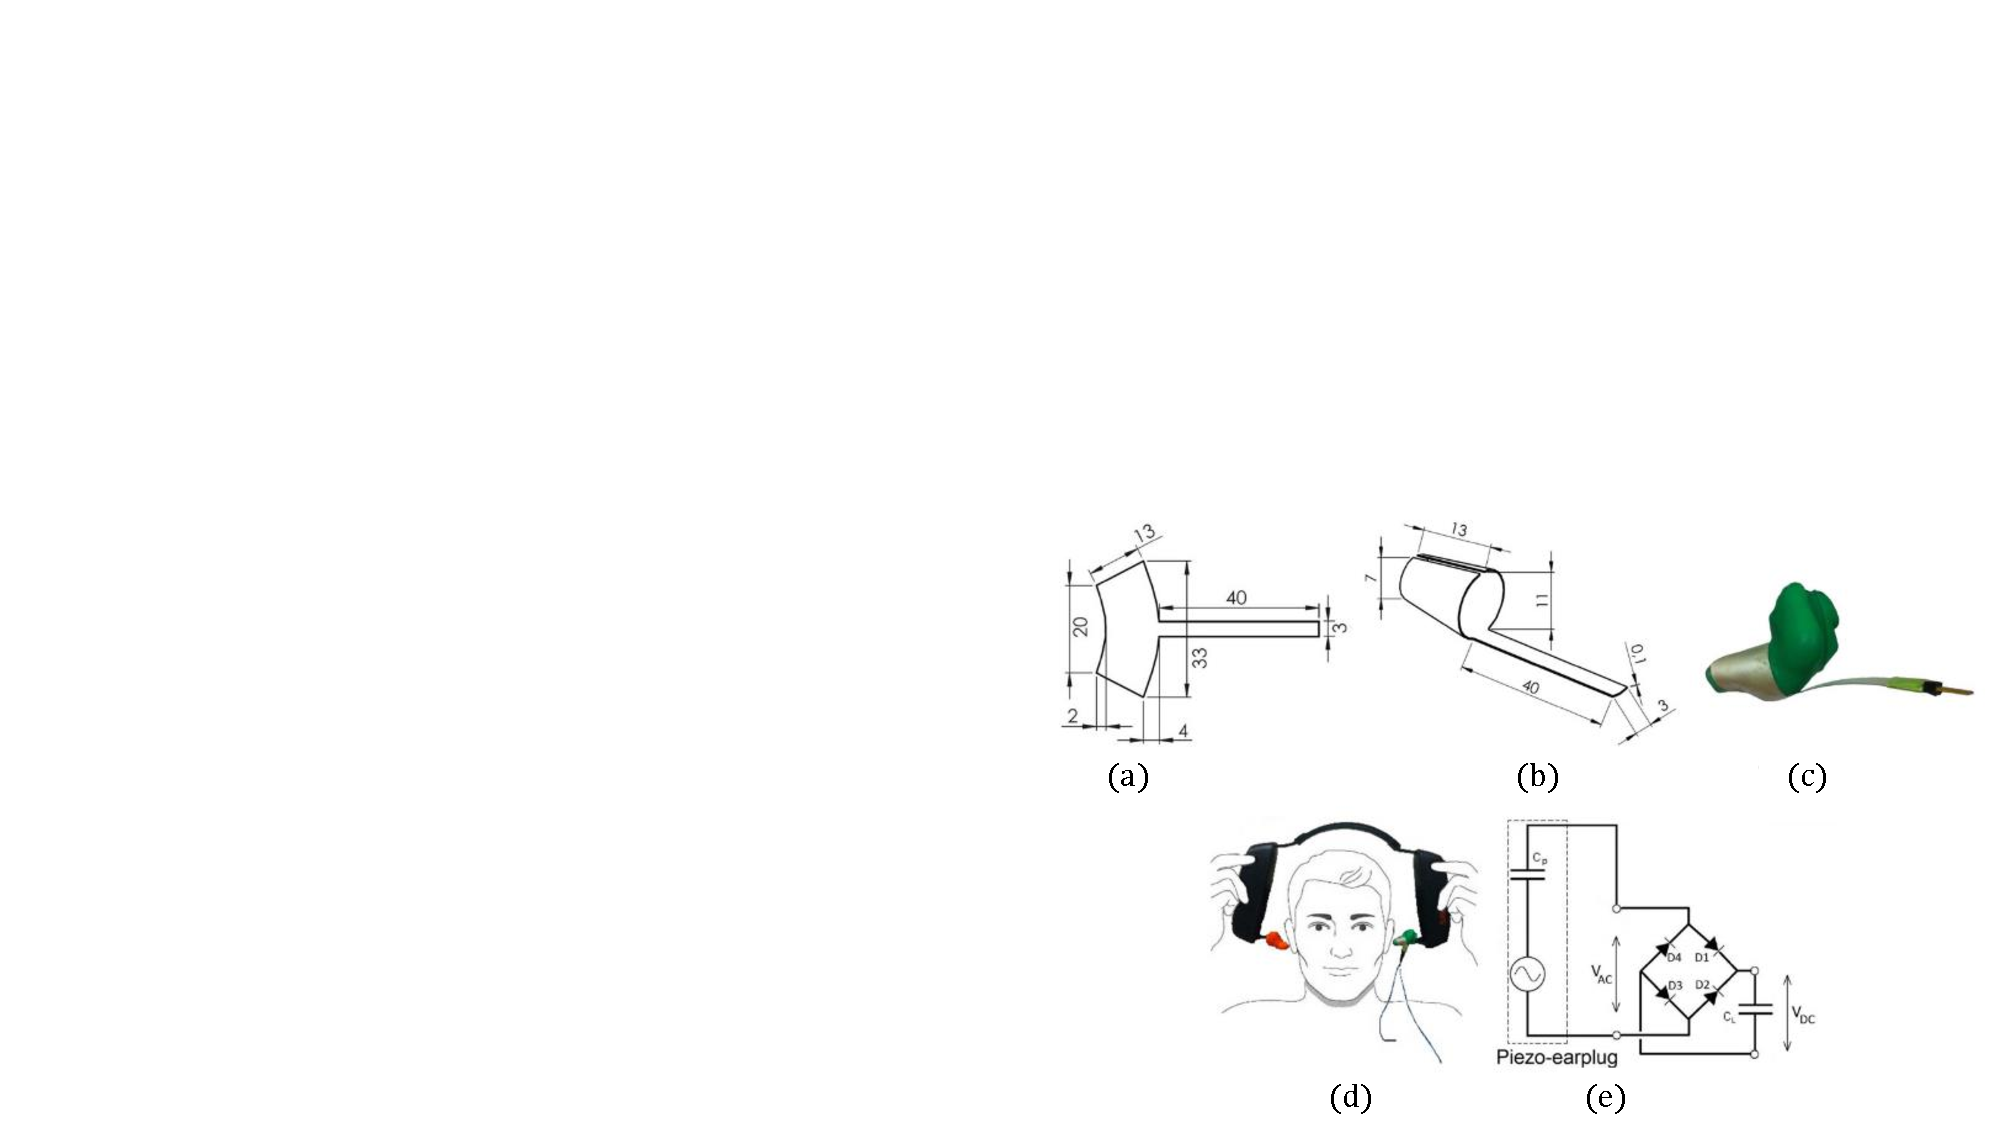
\includegraphics[trim={18cm 0cm 0cm 8.7cm},clip, width=\linewidth]{figures/critias_piezo.pdf}
	\caption{Piezoelectric energy harvester. Experimental setup (dimensions are in mm). (a) Flattened PVDF layer. (b) PVDF layer. (c) Prototype of piezo-earpiece. (d) Piezo-earpiece mounted on the headset. (e) Measuring setup. \cite{Delnavaz2013}}  
	\label{fig:critias_piezo}
\end{figure}
%%%%%%%%%%%%%%%%%%%%%%%%%%%%%%%%%%%%%%%
%%%%%%%%%%%%%%%%%%%%%%%%%%%%%%%%%%%%%%%
\begin{figure}[!htbp]
	\centering
	\captionsetup{justification=centering}
	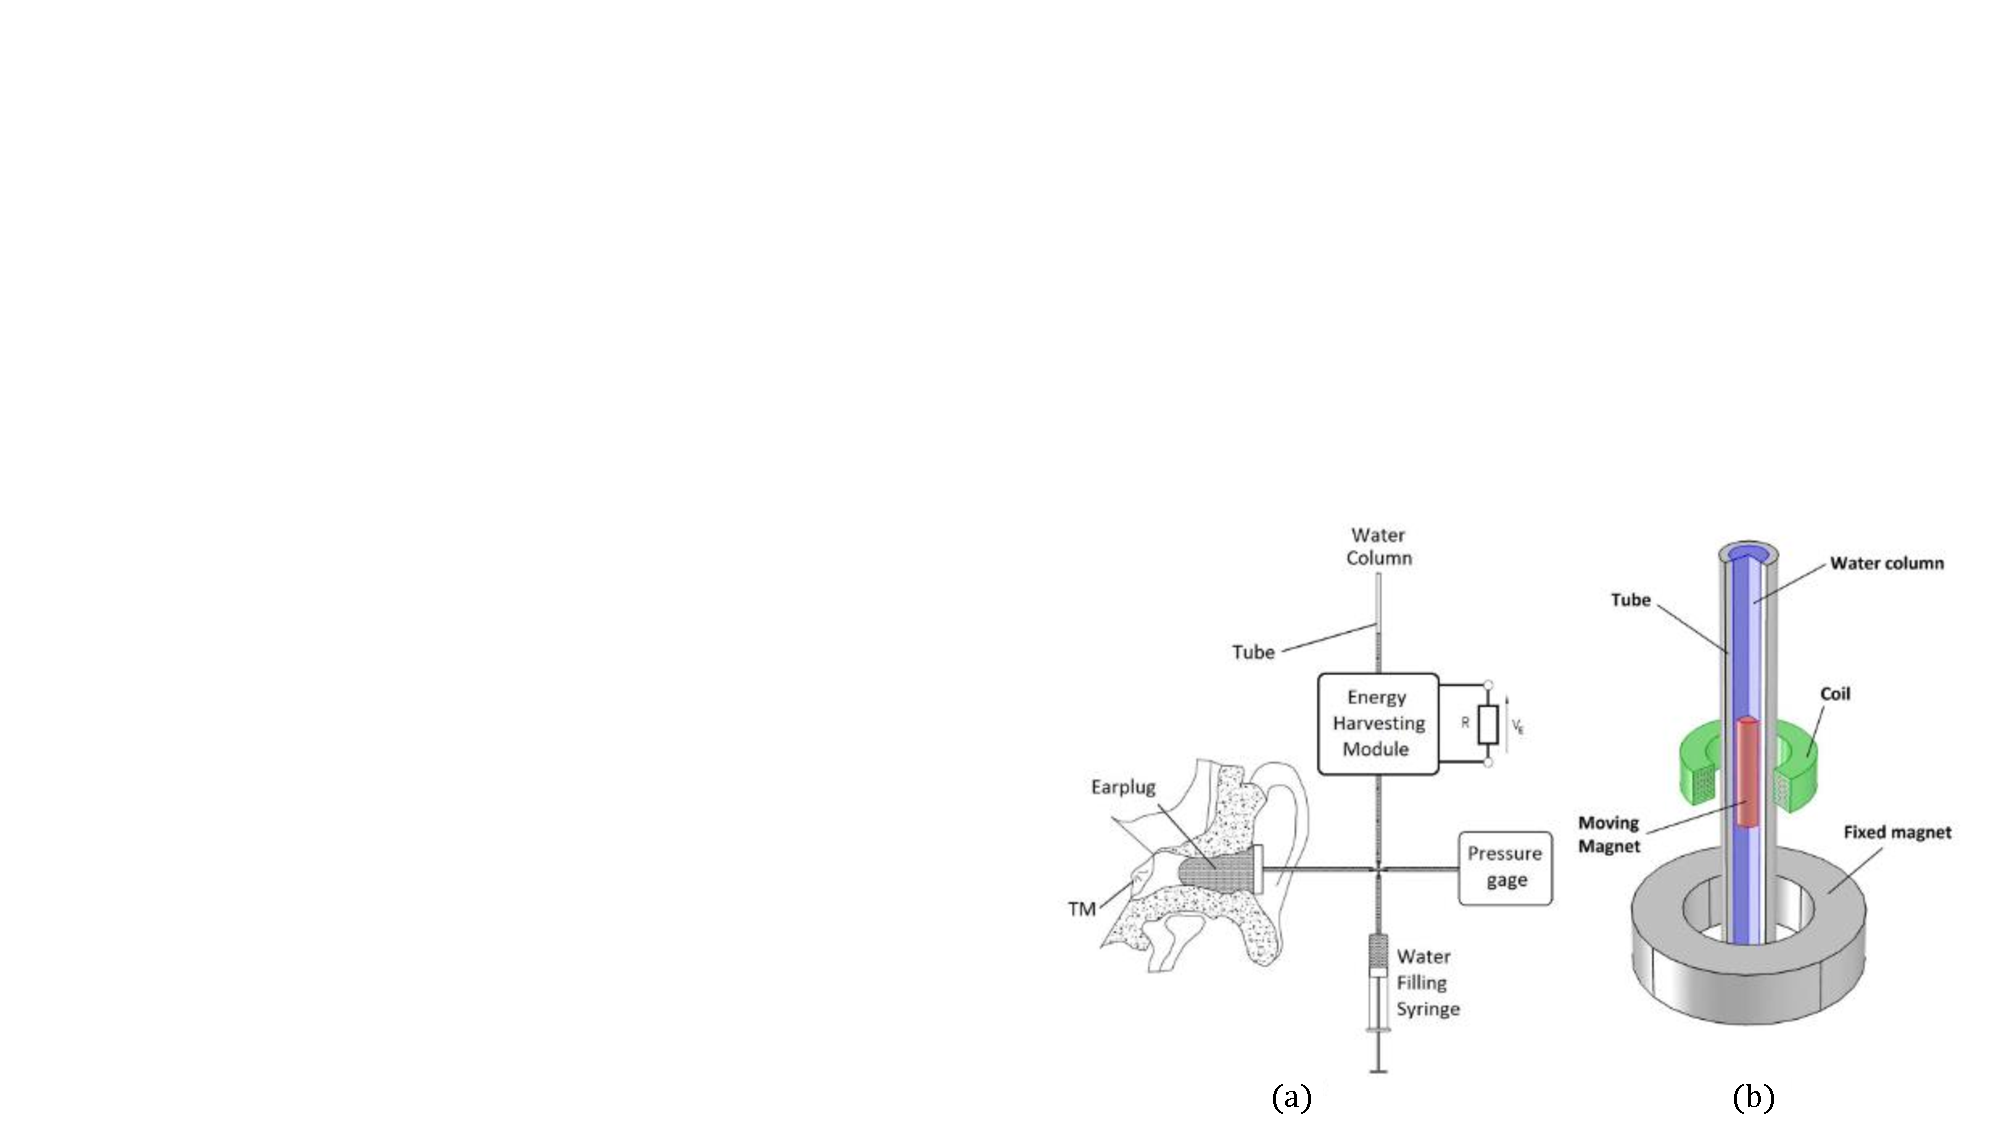
\includegraphics[trim={18cm 0cm 0cm 8.75cm},clip, width=\linewidth]{figures/critias_emag.pdf}
	\caption{Hydroelectromagnetic energy harvester. (a) Test setup. (b) Energy harvesting module. \cite{Delnavaz2012}} 
	\label{fig:critias_emag}
\end{figure}
%%%%%%%%%%%%%%%%%%%%%%%%%%%%%%%%%%%%%%%
%%%%%%%%%%%%%%%%%
\begin{table}[!htbp]
	\centering
	\captionsetup{justification=centering}
	\resizebox{\linewidth}{!}{%
	\begin{tabular}{ l  c  c  c}
		\toprule
		\multicolumn{1}{l}{\textbf{Harvester}}                        &
		\multicolumn{1}{c}{\textbf{Harvested energy per mastication}} &
		\multicolumn{1}{c}{\textbf{Reference}}                        \\
		\midrule
		Piezo earpiece        & $44$µJ 		 & \cite{Delnavaz2013} \\
	    Hydroelectromagnetic  & $0.2$µJ      & \cite{Delnavaz2012} \\
		Piezo sensor          & $0.1$µJ      & \cite{Carioli2018}  \\
		\bottomrule
	\end{tabular}}
	\caption{Existing harvesters exploiting the ear canal deformation energy}
	\label{tab:harvesters_ear}
\end{table}
%%%%%%%%%%%%%%%%%%%%%  
Based on the literature, we propose a new technological solution optimizing the energy conversion efficiency to maximize the harvested energy from the ear canal dynamic motion. Section \ref{sec:HARVESTER PRESENTATION AND OPERATION PRINCIPLE} presents the harvester and describes its operation principle. Section \ref{sec:SYSTEM MODELING AND SIMULATIONS} shows the global system  modeling and the numerical simulation on its behavior. Then section \ref{sec:EXPERIMENTAL CHARACTERIZATIONS} then exposes the experimental validation performed on the harvester critical components and section \ref{sec:MODEL RECALIBRATION WITH EXPERIMENTAL DATA} presents the experimentally adjusted global harvester model. Section \ref{sec:ANALYZE AND DISCUSSION} discusses this work major contributions and the harvester potential. Finally, a conclusion is stated in the last section.

%/!\/!\/!\/!\/!\/!\/!\/!\/!\/!\/!\/!\/!\/!\/!\/!\/!\/!\/!\/!\/!\/!\/!\/!\%
\section{HARVESTER PRESENTATION AND OPERATION \mbox{PRINCIPLE}}
\label{sec:HARVESTER PRESENTATION AND OPERATION PRINCIPLE}
%/!\/!\/!\/!\/!\/!\/!\/!\/!\/!\/!\/!\/!\/!\/!\/!\/!\/!\/!\/!\/!\/!\/!\/!\%
%%%%%%%%%%%%%%%%%%%%%%%%%%%%%%%%%%%%%%%
\begin{figure*}[!htbp]
	\centering
	\captionsetup{justification=centering}
	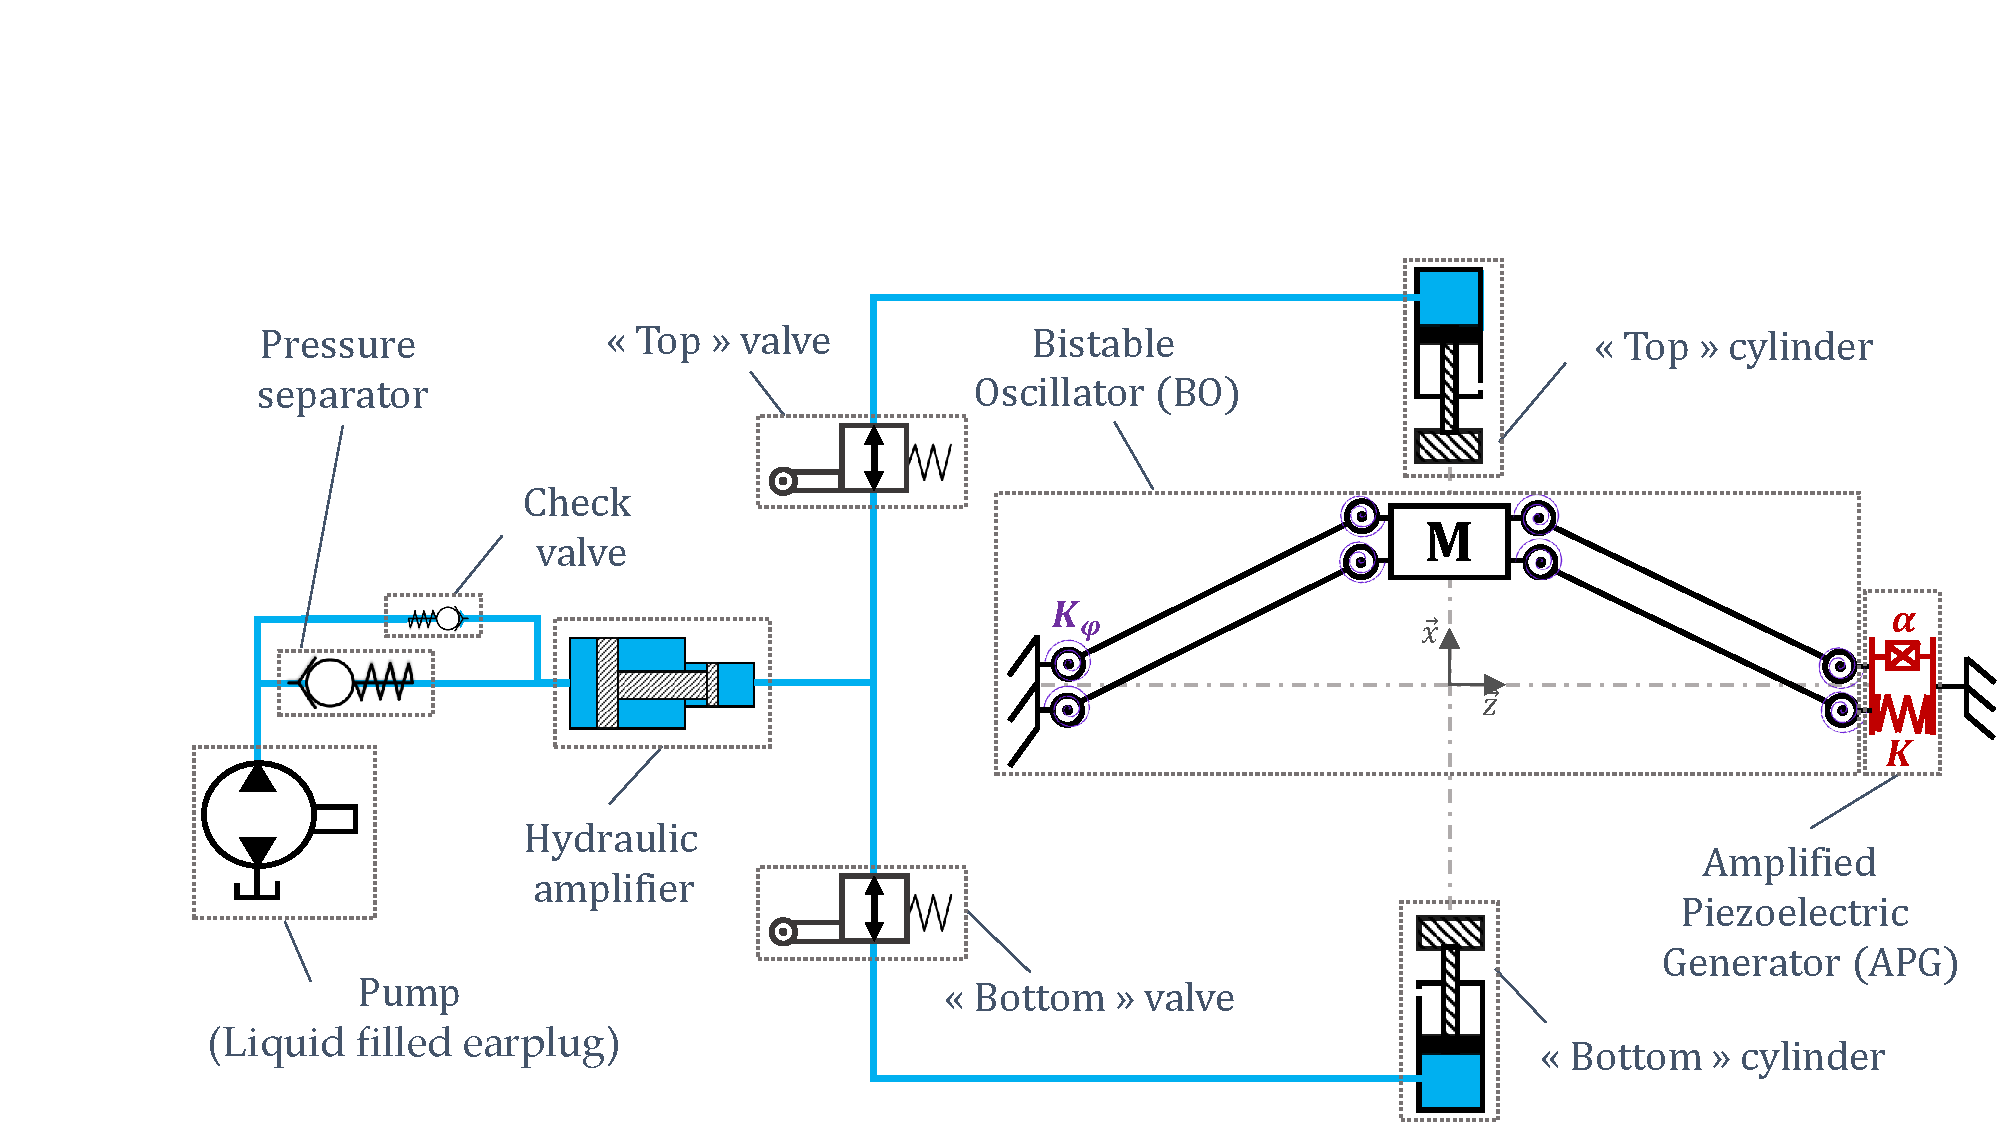
\includegraphics[trim={3.2cm 0cm 0cm 4.3cm},clip, width=0.7\textwidth]{figures/system_presentation.pdf}
	\caption{Schematic presentation of the frequency-up piezoelectric harvester exploiting the ear canal geometry variation} 
	\label{fig:system_presentation}
\end{figure*}
%%%%%%%%%%%%%%%%%%%%%%%%%%%%%%%%%%%%%%%
The figure \ref{fig:system_presentation} presents a schematic view of the energy harvesting system. It uses a liquid filled earplug to transmit the energy outside the ear canal and benefit so from larger effective space. To maximize the efficiency, the system integrates a frequency-up conversion stage performed by a bistable oscillator (BO). The latter implements an amplified piezoelectric generator (APG) made of a flextensional elastic APX4 steel structure containing stacked lead zirconate titanate (PZT) ceramics (fig. \ref{fig:APG}). The electromechanical converter composed of the BO and the APG theoretically offers higher energy conversion efficiency compared to low frequency solutions and/or flexible electromechanical transducers \cite{Guo2019,Peng2021,Kulah2008}.
%%%%%%%%%%%%%%%%%%%%%%%%%%%%%%%%%%%%	
\begin{figure}[!htb]
	\begin{center}
		\begin{subfigure}[t]{0.6\linewidth}
			\captionsetup{justification=centering}
			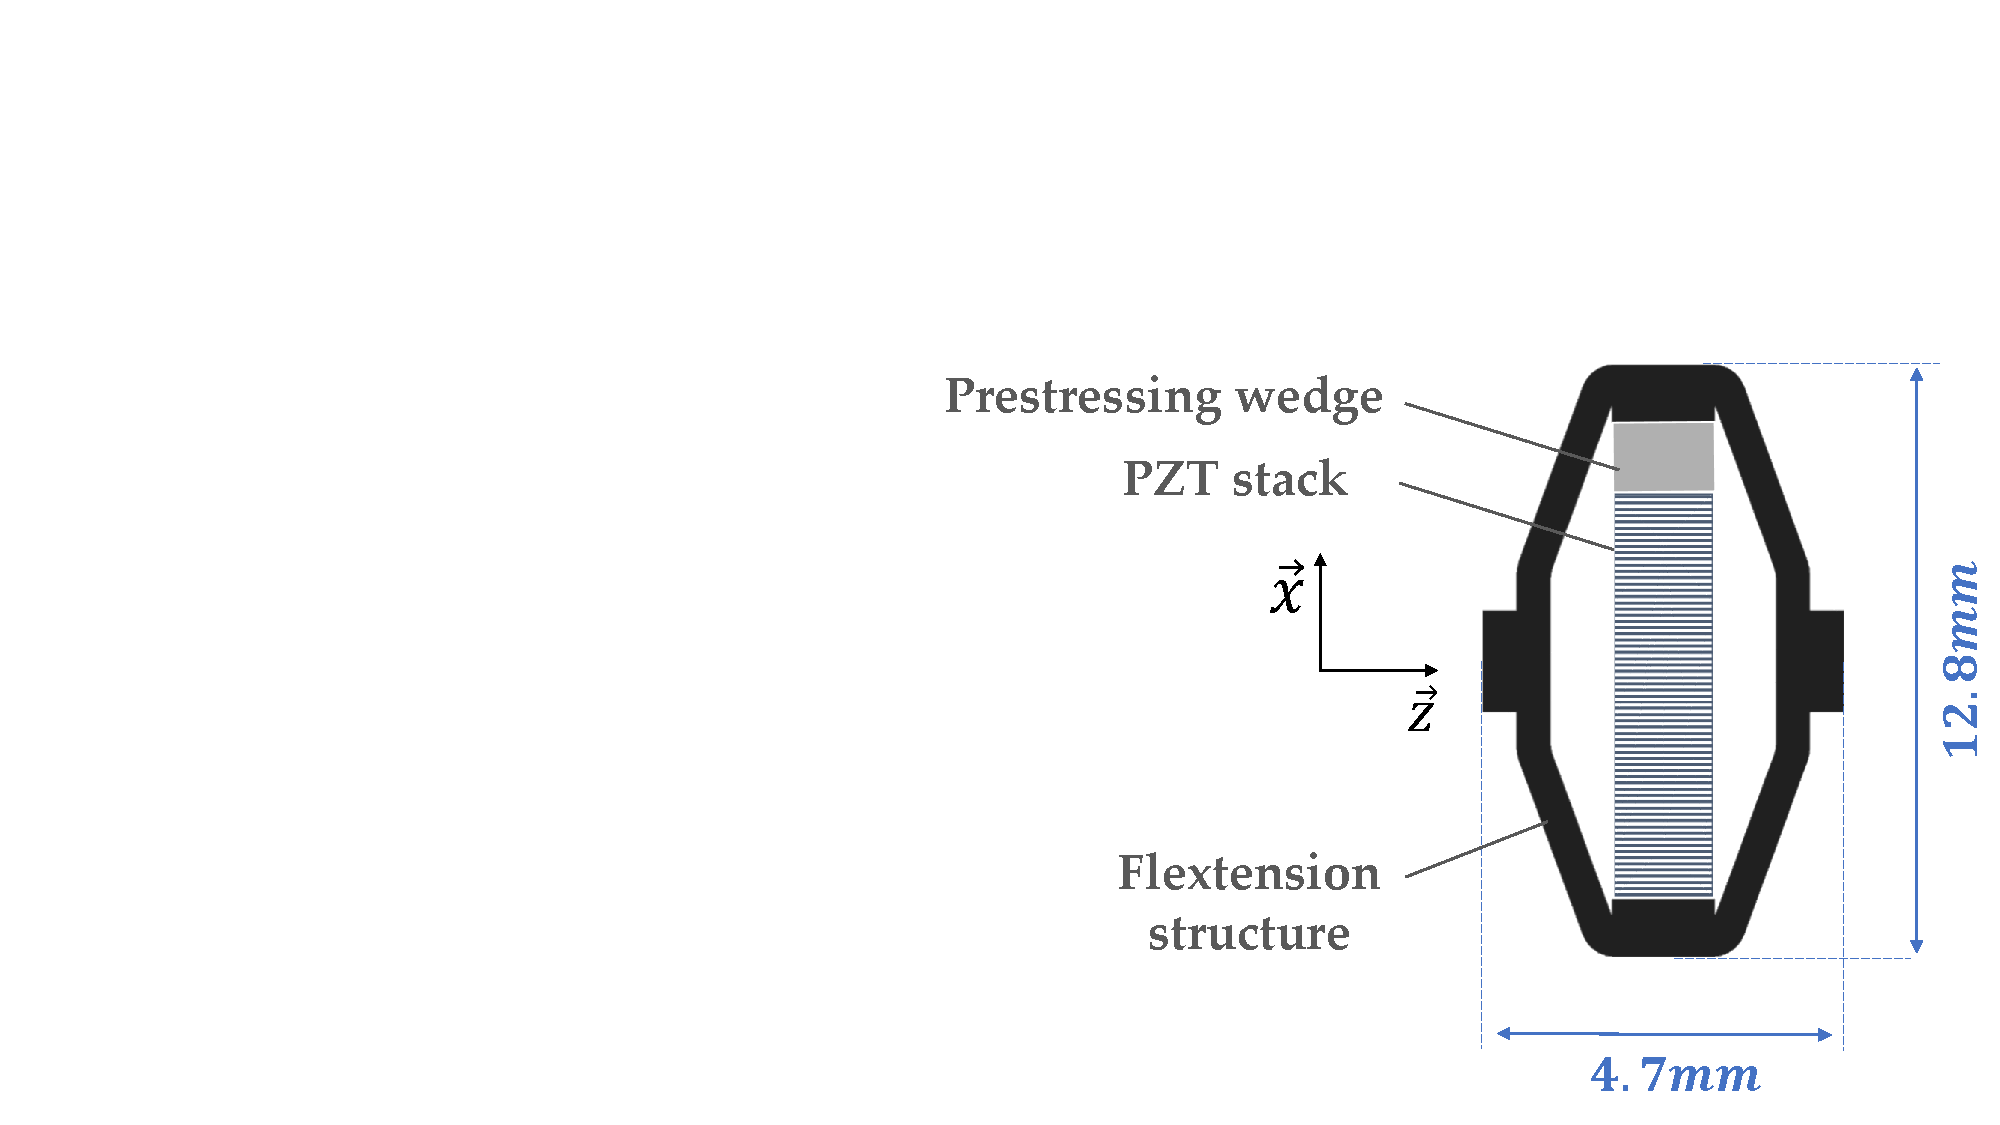
\includegraphics[trim={16cm 0cm 0cm 6cm},clip,width=\linewidth]{figures/APG_schema.pdf}
			\caption{Detailed schema}
			\label{fig:APG_schema}
		\end{subfigure}
		\hfillx
		\begin{subfigure}[t]{0.29\linewidth}
			\captionsetup{justification=centering}
			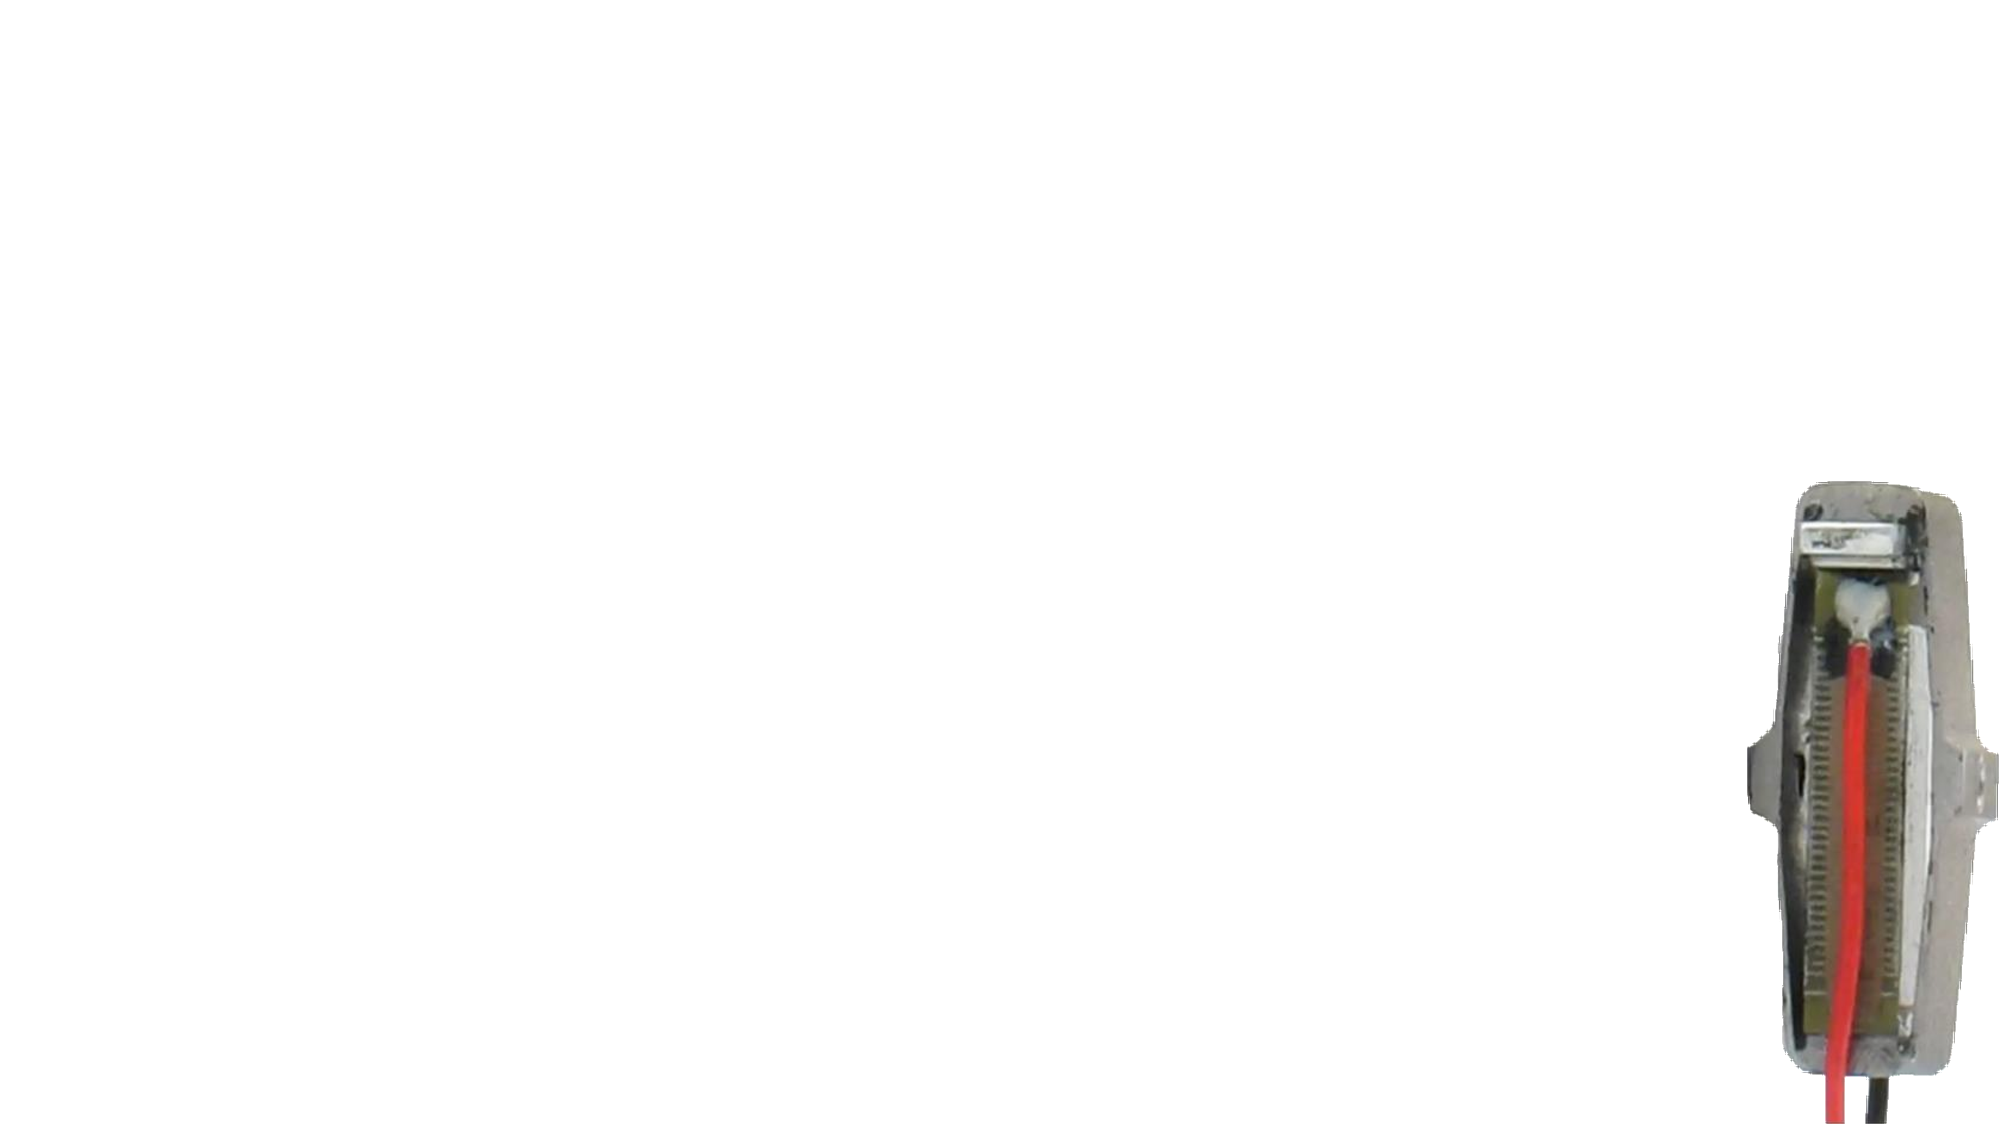
\includegraphics[trim={29.5cm 0cm 0cm 8cm},clip,width=0.65\linewidth]{figures/APG_photo.pdf}
			\caption{Picture}
			\label{fig:APG_photo}
		\end{subfigure}
		\caption{The APG presentation}
		\label{fig:APG}
	\end{center}
\end{figure}
%%%%%%%%%%%%%%%%%%%%%%%%%%%%%%%%%%%% 

The electromechanical converter is actuated, by two hydraulic cylinders (HC), with the hydraulic energy transmitted from the liquid filled earplug, through a pressure separator, a hydraulic amplifier and two hydraulic valves (HV).

To maximize the mechanical energy transfer between the ear canal and the earplug, the latter is lightly pressurized. A minimum of 14kPa is needed in order to fit the earplug to the ear canal wall \cite{Delnavaz2013}. The pressure separator ensures that this initial pressurization does not interfere on the system operation. Then, during a mastication cycle, the TMJ compresses the ear canal wall and expels so the fluid outside the earplug. The HVs ensure to led the fluid alternatively to each HC in order to actuate the BO mass back and forward. The hydraulic amplifier adapts the cylinders stroke to the available earplug flow rate and also adapts the mechanical impedance of the BO to the mechanical impedance of the ear canal wall.

The BO mass has two stable equilibrium positions, $x_m = x_0$ and $x_m = -x_0$. The harvester operates on two major phases. The first consists on the BO mass actuation, by a HC, from one stable equilibrium position toward the unstable position at $x_m = 0$. During the second phase the mass goes oscillate around the opposite stable equilibrium position until it stops, while a portion of the oscillatory energy is converted in electricity by the GPA. The mass then moves backward during the next mastication, completing so the harvester cycle.
%%%%%%%%%%%%%%%%%%%%%%%%%%%%%%%%%%%%%%%
\begin{figure}[!htbp]
	\centering
	\captionsetup{justification=centering}
	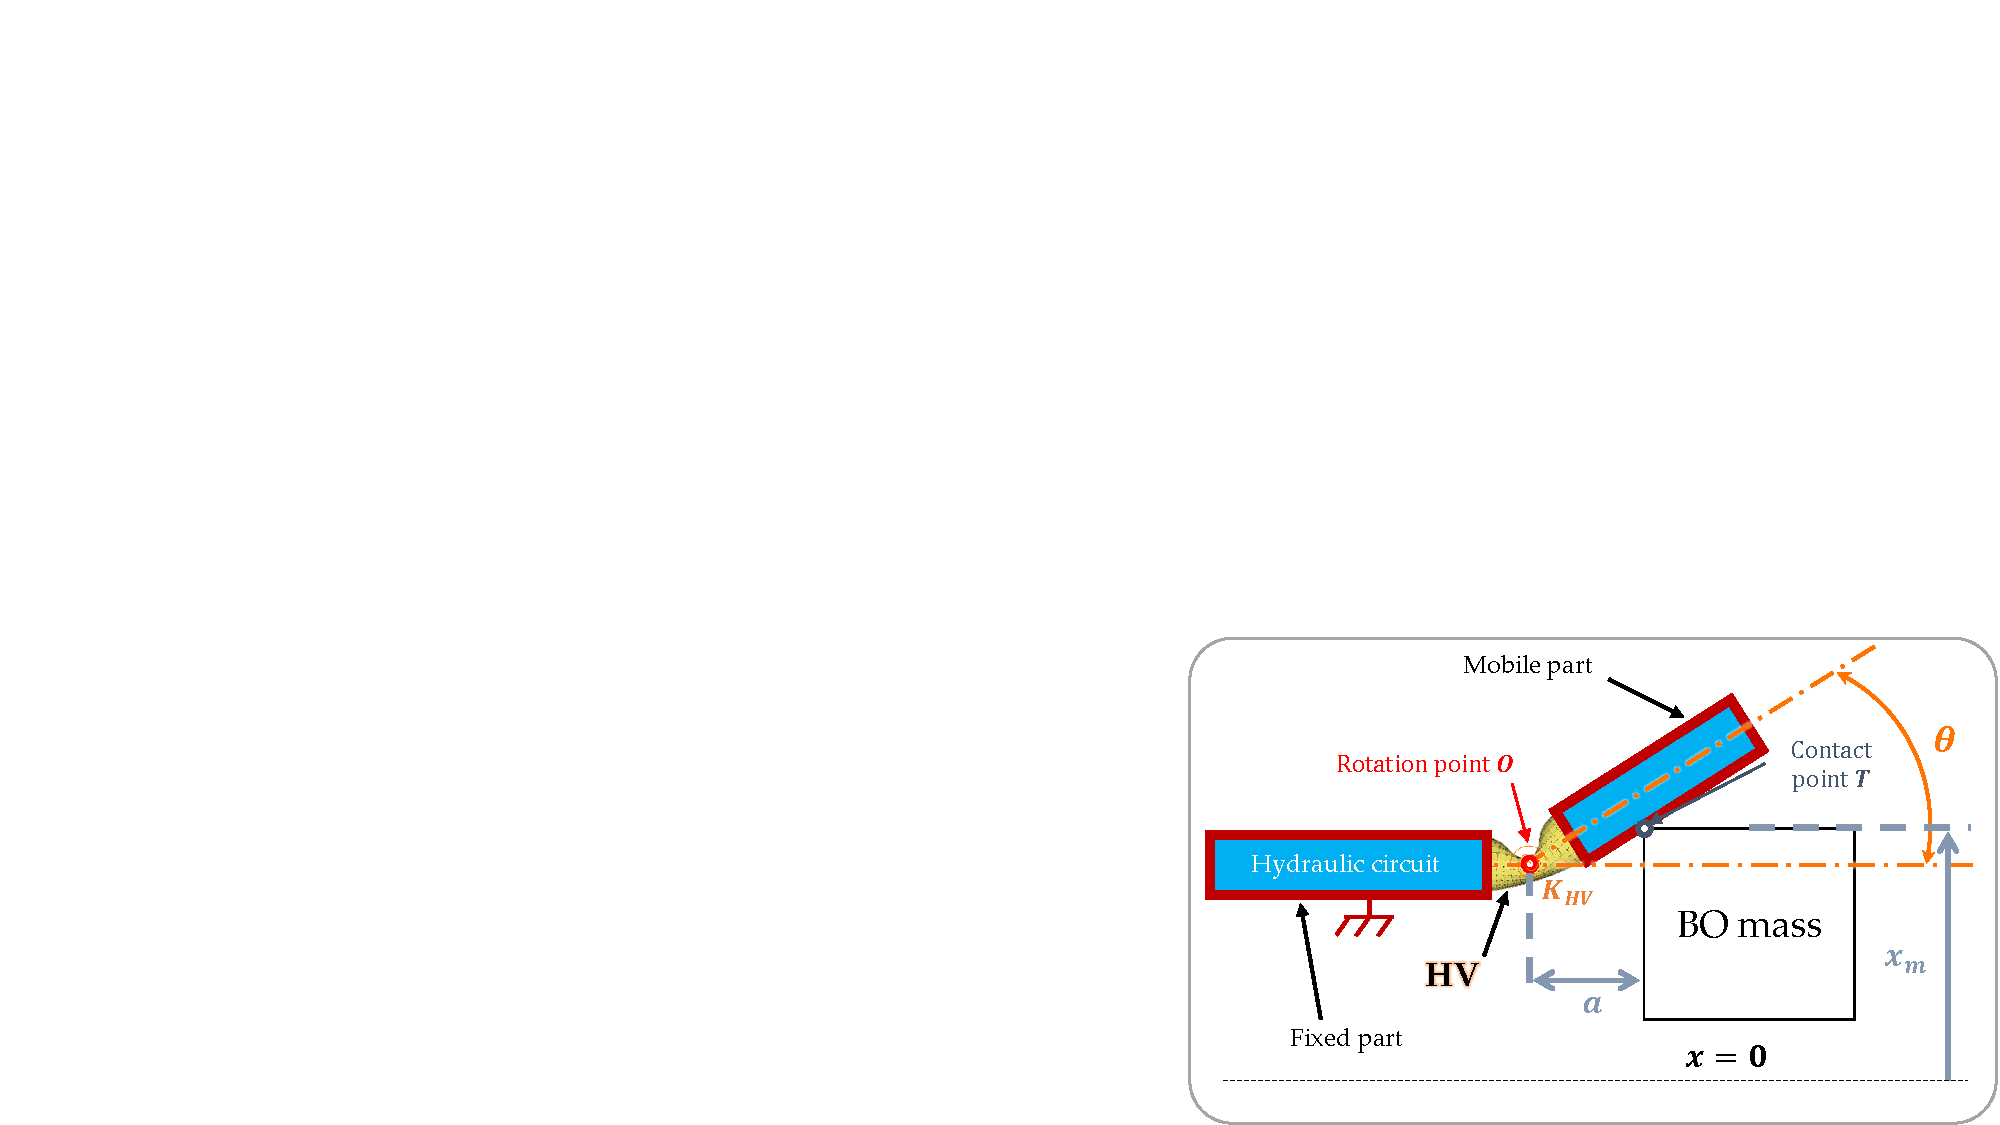
\includegraphics[trim={20cm 0cm 0cm 10.75cm},clip, width=\linewidth]{figures/HV_actuation_detail.pdf}
	\caption{Contact detail between a HV and the BO mass} 
	\label{fig:HV_actuation_detail}
\end{figure}
%%%%%%%%%%%%%%%%%%%%%%%%%%%%%%%%%%%%%%%

In order to maximize the harvested energy we must minimize the energy consumed by the HVs. A technological solution for this role is to use a flexible tube buckled by bending. The figure \ref{fig:HV_actuation_detail} schematizes the integration of such HV around the BO environment. The valve is composed of a flexible tube connected between a rigid part of the hydraulic circuit and a fixed one. The BO mass motion on the mobile part induces a bending angle $\theta$ around the rotational point $O$ located at the buckled section of the flexible tube. Consequently, a pressure loss is generated through the valve in buckled position. Thus, a HV is considered closed when the BO mass is at a stable equilibrium position ($x_m=\pm x_0$) and opened when the mass is at $x_m=0$. Two HVs symmetrically placed on each side of the $\vec{x}$ axis set up an opened hydraulic circuit on one side and a closed one on the other side, depending on the BO mass position. The HV technological choice is motivated by three major arguments. First, the absence of electromechanical transduction minimizes the energy losses for the valve operation. Then, the post-buckling softening of the bent tube minimizes the mechanical impact on the BO mass dynamic operation. Finally, it is well adapted at the millimetric application scale.

%/!\/!\/!\/!\/!\/!\/!\/!\/!\/!\/!\/!\/!\/!\/!\/!\/!\/!\/!\/!\/!\/!\/!\/!\%
\section{SYSTEM GLOBAL MODELING AND SIMULATIONS}
\label{sec:SYSTEM MODELING AND SIMULATIONS}
%/!\/!\/!\/!\/!\/!\/!\/!\/!\/!\/!\/!\/!\/!\/!\/!\/!\/!\/!\/!\/!\/!\/!\/!\%
The harvester is a multyphisic system composed of hydraulic, mechanical, and electrical components. This section presents a global multiphysic model describing the theoretical system operation. Two coupled subsystems are considered. The subsection \ref{subsec:The electromechanical converter} shows the modeling of the electromechanical frequency-up converter (BO + APG) under the mechanical influence of a HV and a HC. Then, the subsection \ref{subsec:The hydraulic circuit} discusses the design of the hydraulic circuit composed of the two HVs, the two HCs, the hydraulic amplifier, the pressure separator and the liquid filled earplug. Finally, the section \ref{subsec:Global model simulation} exposes the numerical simulation of the designed multiphysic coupled model.

    %///////////////////////////////////////////// 
	\subsection{The electromechanical converter}	
	\label{subsec:The electromechanical converter}
    %/////////////////////////////////////////////

%%%%%%%%%%%%%%%%%%%%%%%%%%%%%%%%%%%%%%
\begin{figure*}[!htbp]
	\centering
	\captionsetup{justification=centering}
	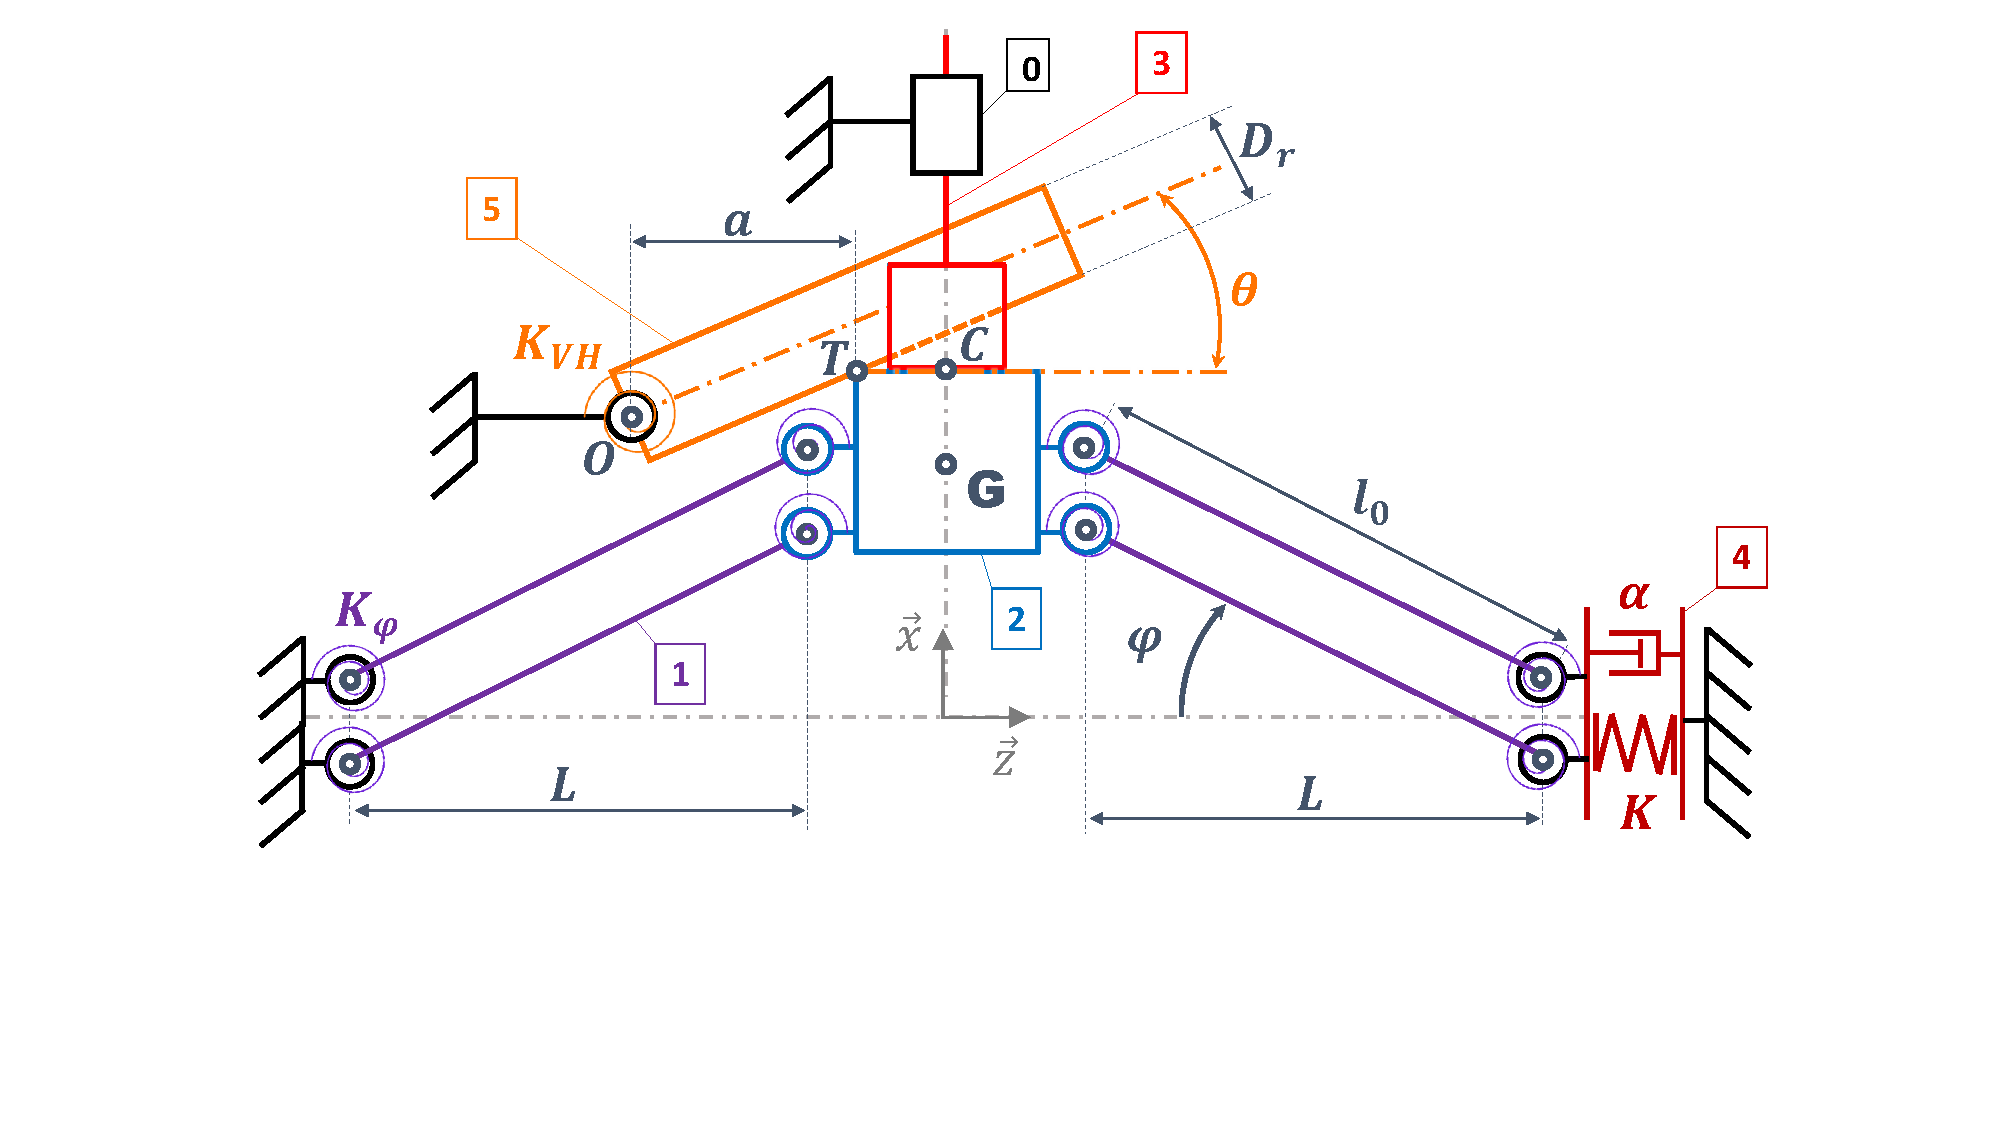
\includegraphics[trim={0cm 0cm 0cm 0cm},clip, width=0.9\textwidth]{figures/schema_cinematique1.pdf}
	\caption{Schema système complet.}
	\label{fig:schema_cinematique1}
\end{figure*}
%%%%%%%%%%%%%%%%%%%%%%%%%%%%%%%%%%%%%%


    %///////////////////////////////////////////// 
	\subsection{The hydraulic circuit}	
	\label{subsec:The hydraulic circuit}
    %/////////////////////////////////////////////

	%///////////////////////////////////////////// 
	\subsection{Global model simulation}	
	\label{subsec:Global model simulation}
	%/////////////////////////////////////////////

\lipsum[1]
%%%%%%%%%%%%%%%%%%%%%%%%%%%%%%%%%%%%%%
\begin{figure}[!htbp]
	\centering
	\captionsetup{justification=centering}
	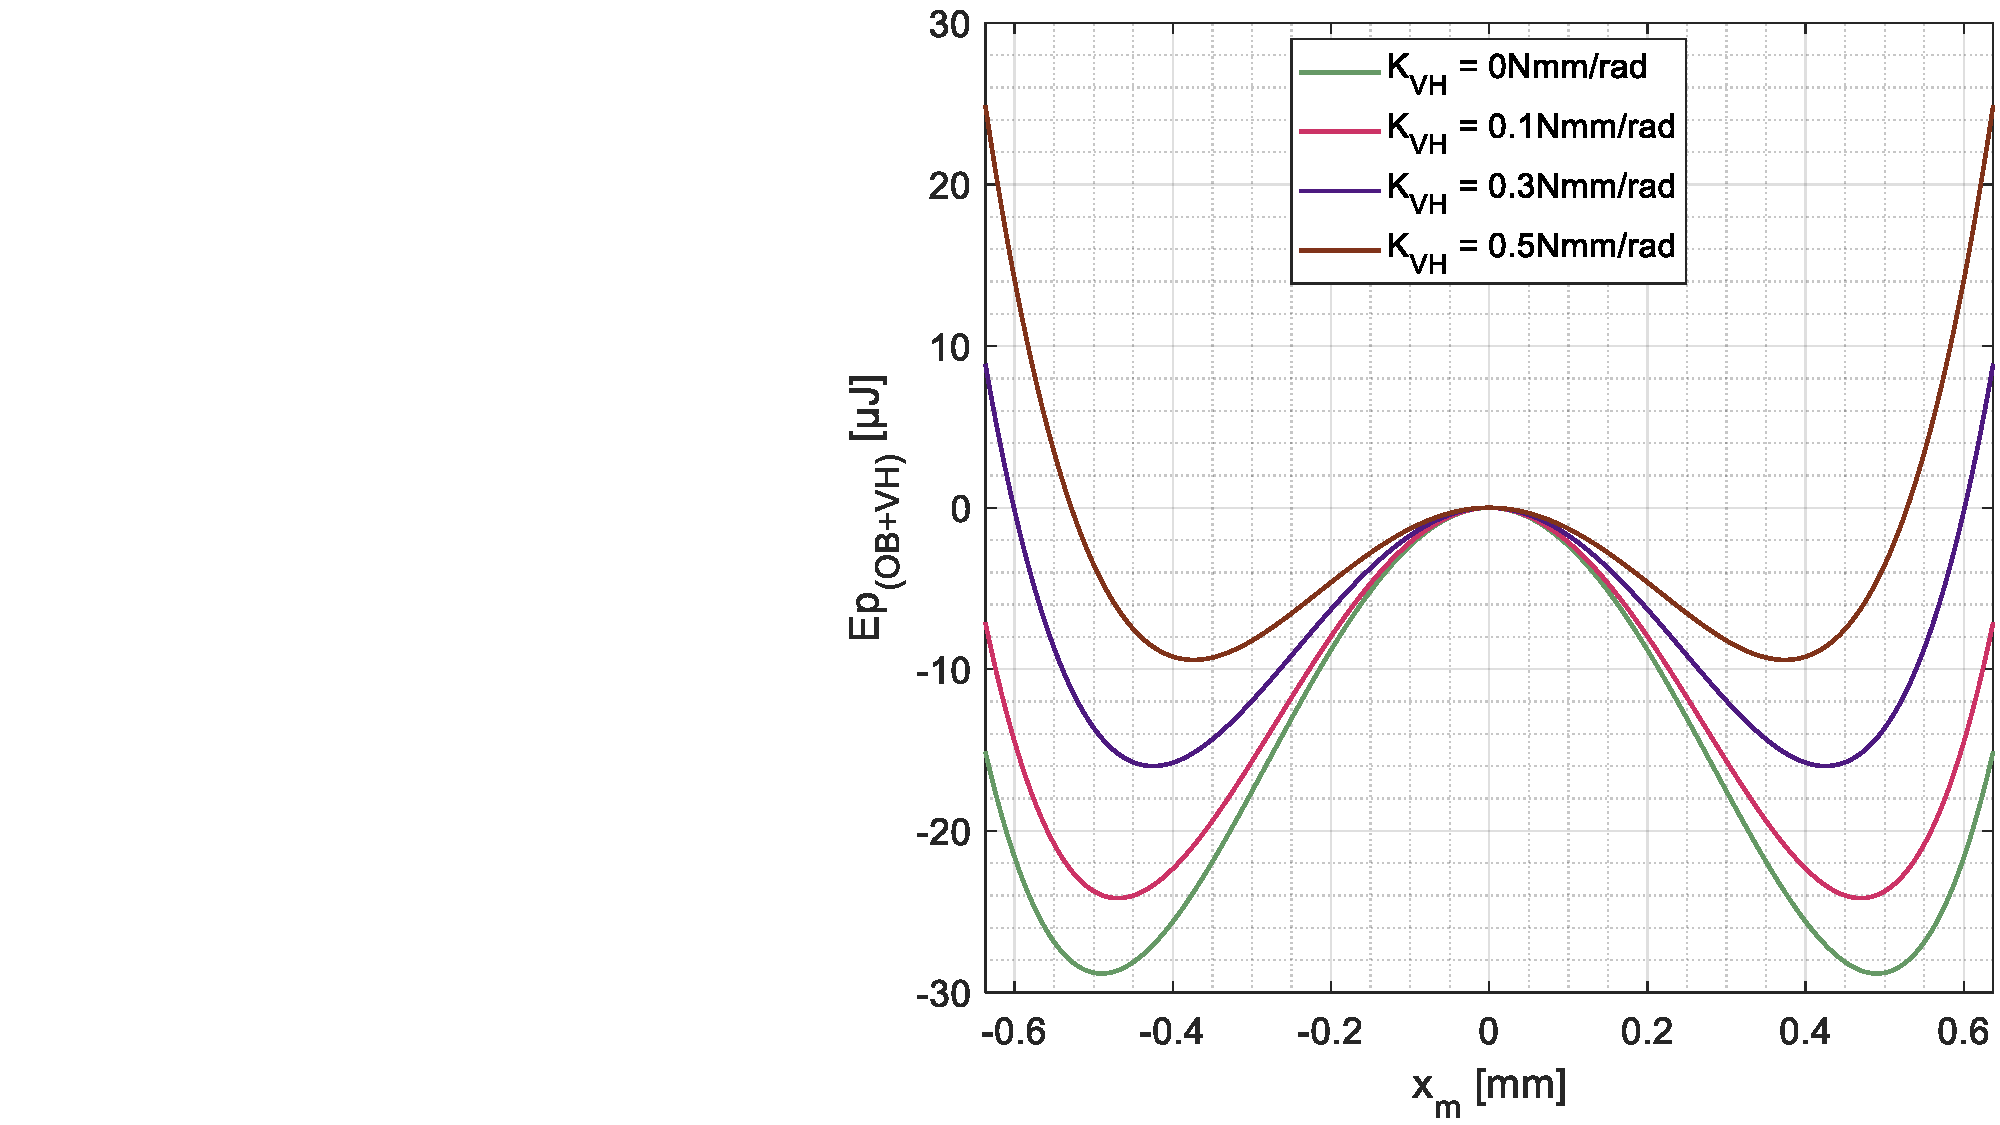
\includegraphics[trim={14cm 0cm 0cm 0cm},clip, width=0.49\textwidth]{figures/(Ep)_vs_(x_m)_avec_plusieurs_K_VH.pdf}
	\caption{$K_{HV}$ impact on the evolution of the BO mass potential energy.}
	\label{fig:(Ep)_vs_(x_m)_avec_plusieurs_K_VH}
\end{figure}
%%%%%%%%%%%%%%%%%%%%%%%%%%%%%%%%%%%%%%%

%%%%%%%%%%%%%%%%%%%%%%%%%%%%%%%%%%%%%%
\begin{figure}[!htbp]
	\centering
	\captionsetup{justification=centering}
	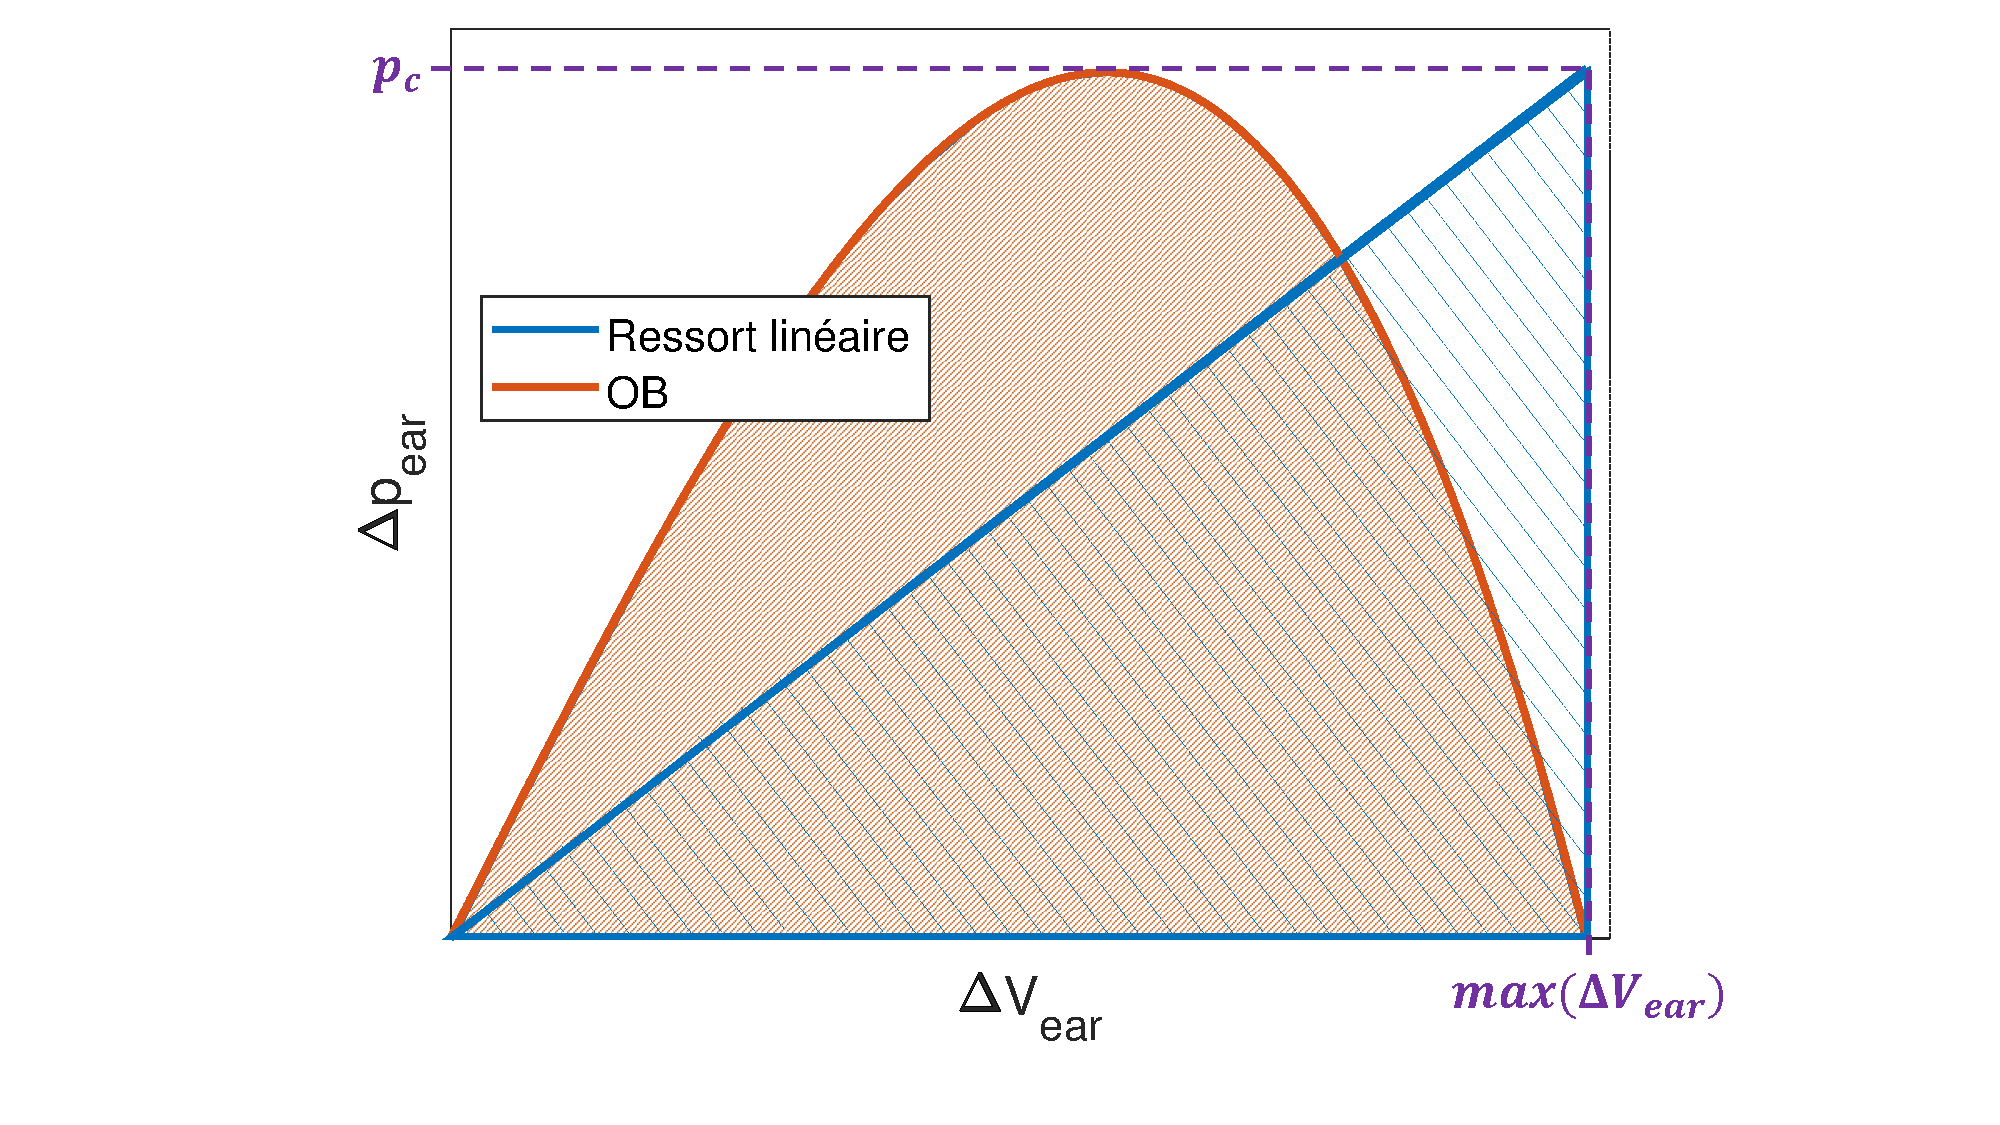
\includegraphics[trim={6cm 1cm 4cm 0.5cm},clip, width=0.49\textwidth]{figures/force_elastique_lineaire_vs_OB.pdf}
	\caption{Schema système complet.}
	\label{fig:force_elastique_lineaire_vs_OB}
\end{figure}
%%%%%%%%%%%%%%%%%%%%%%%%%%%%%%%%%%%%%%
%/!\/!\/!\/!\/!\/!\/!\/!\/!\/!\/!\/!\/!\/!\/!\/!\/!\/!\/!\/!\/!\/!\/!\/!\%
\label{NUMERICAL MODEL AND SIMULATIONS}
%/!\/!\/!\/!\/!\/!\/!\/!\/!\/!\/!\/!\/!\/!\/!\/!\/!\/!\/!\/!\/!\/!\/!\/!\%
\lipsum[1]
%%%%%%%%%%%%%%%%%%%%%%%%%%%%%%%%%%%%%%
\begin{figure*}[!htbp]
	\centering
	\captionsetup{justification=centering}
	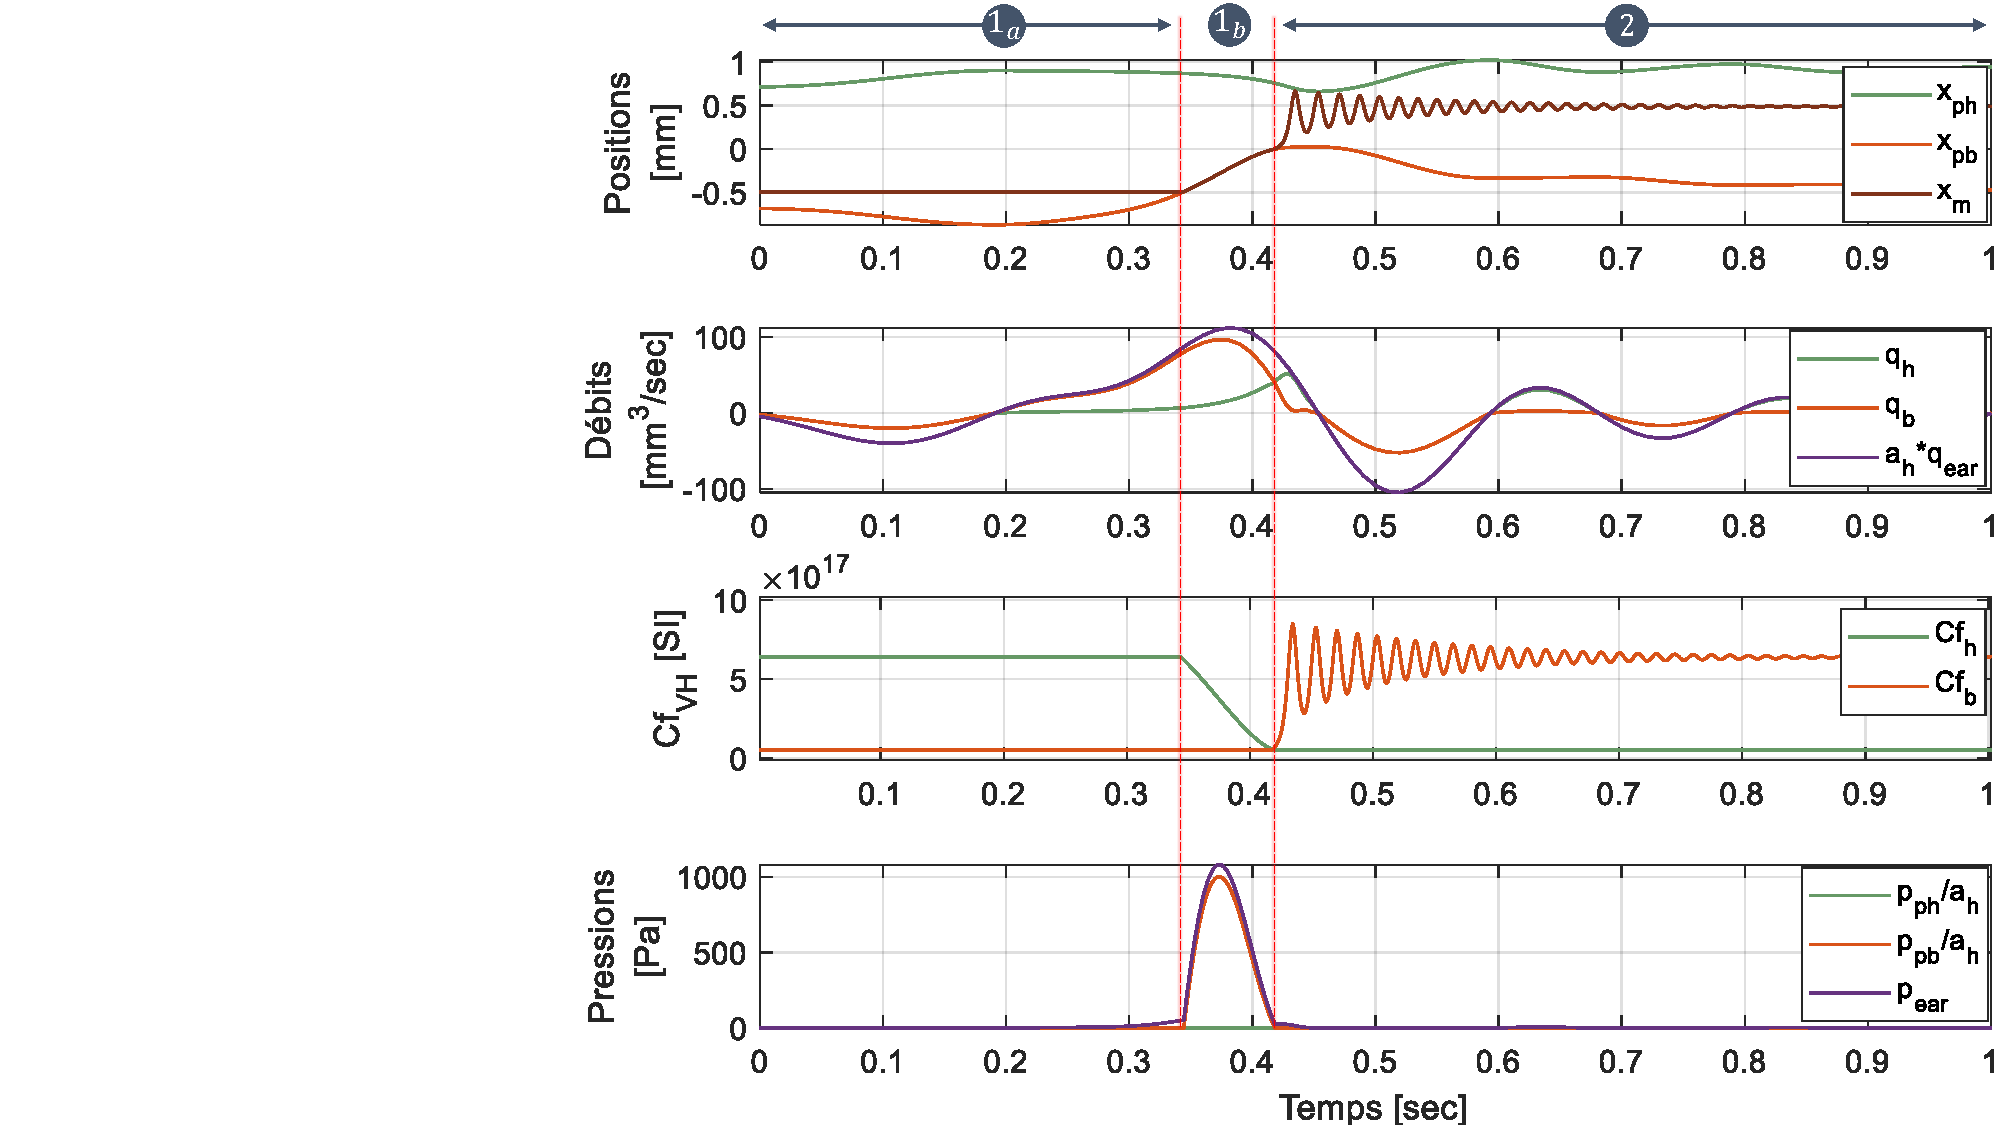
\includegraphics[trim={9.5cm 0cm 0cm 0cm},clip, width=0.7\textwidth]{figures/simu_pos_debit_Cf_pression_1CYCLE.pdf}
	\caption{$K_{HV}$ impact on the evolution of the BO mass potential energy.}
	\label{fig:simu_pos_debit_Cf_pression_1CYCLE}
\end{figure*}
%%%%%%%%%%%%%%%%%%%%%%%%%%%%%%%%%%%%%%%
\lipsum[1]
%%%%%%%%%%%%%%%%%%%%%%%%%%%%%%%%%%%%%%
\begin{figure*}[!htbp]
	\centering
	\captionsetup{justification=centering}
	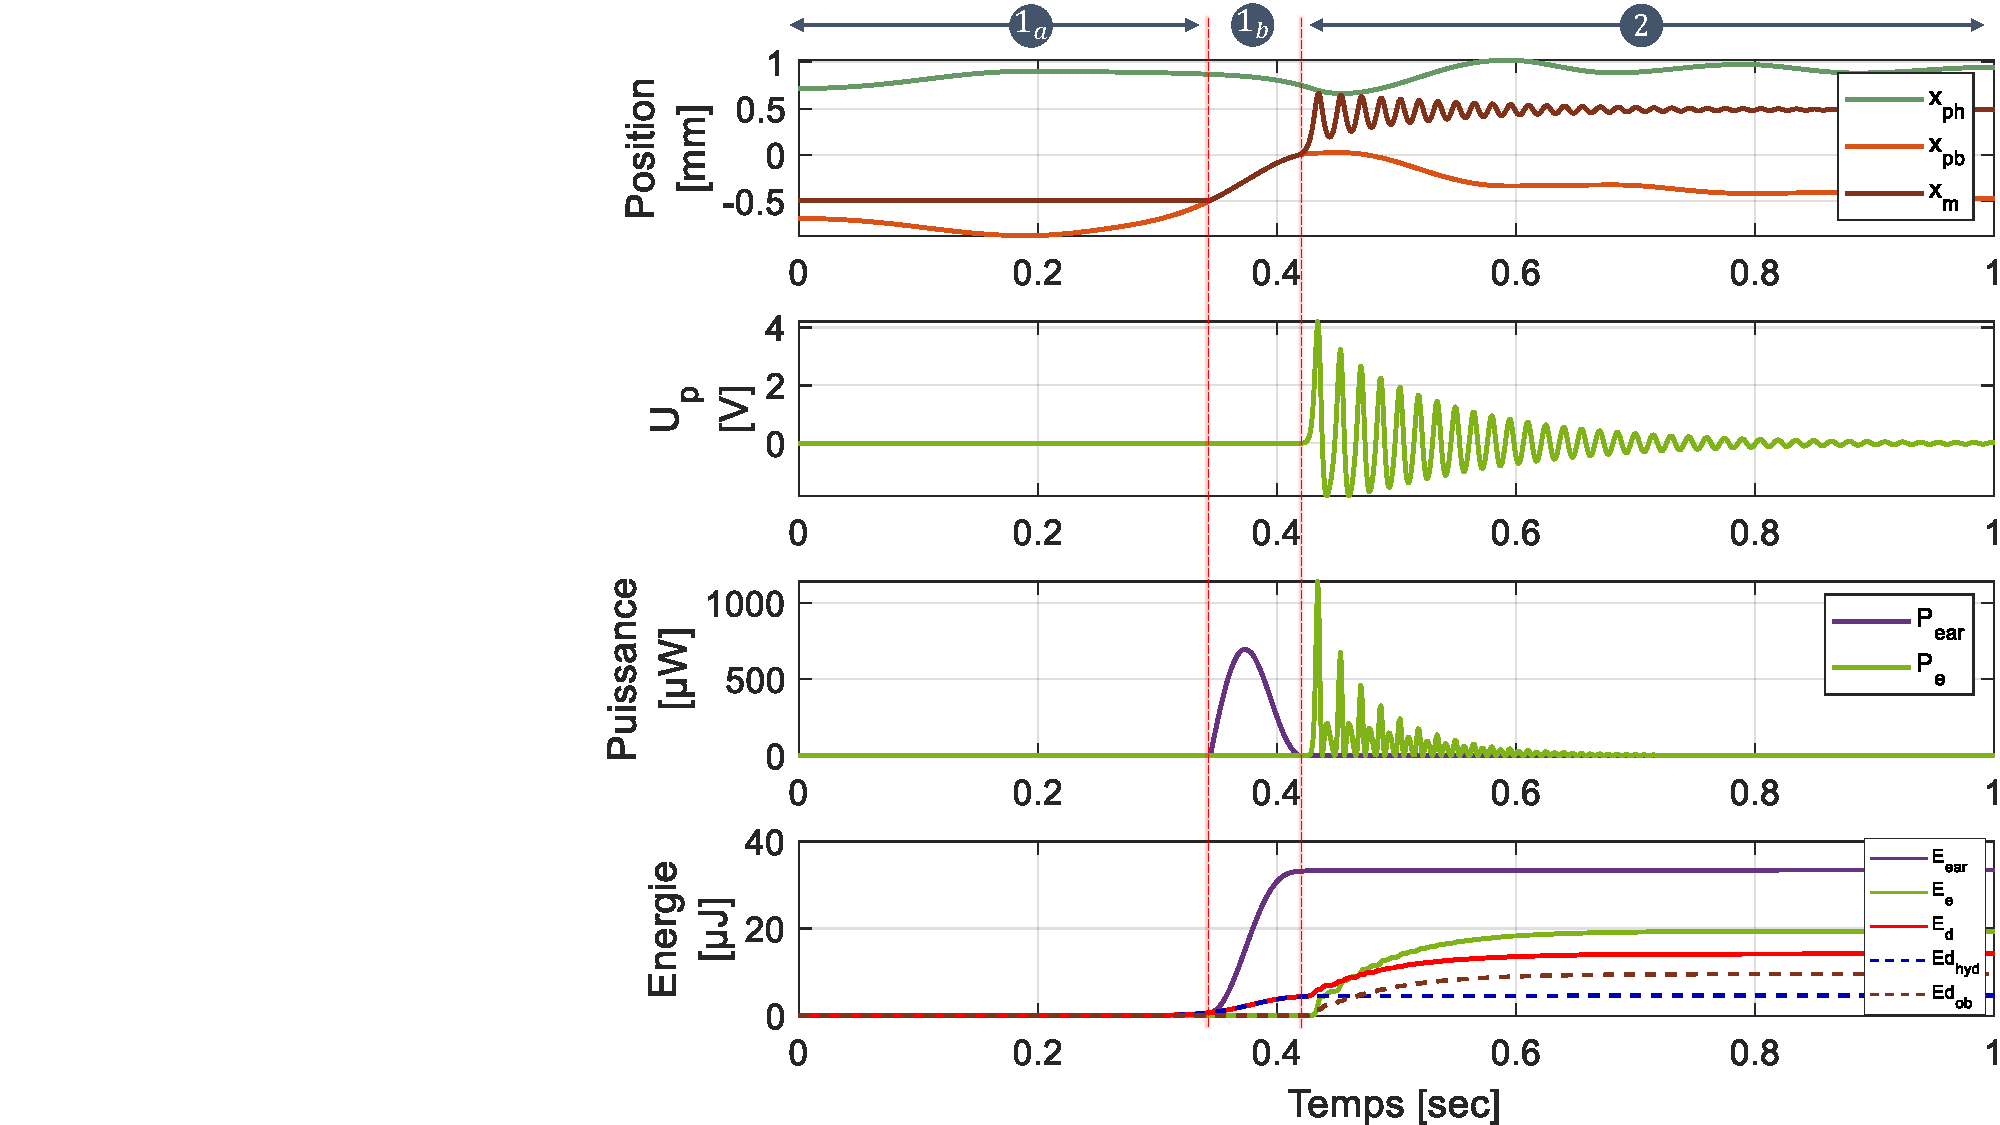
\includegraphics[trim={10cm 0cm 0cm 0cm},clip, width=0.7\textwidth]{figures/simu_pos_Up_puissances_energie_1CYCLE.pdf}
	\caption{$K_{HV}$ impact on the evolution of the BO mass potential energy.}
	\label{fig:simu_pos_Up_puissances_energie_1CYCLE}
\end{figure*}
%%%%%%%%%%%%%%%%%%%%%%%%%%%%%%%%%%%%%%%
%%%%%%%%%%%%%%%%%%%%%%%%%%%%%%%%%%%%%%
\begin{figure*}[!htbp]
	\centering
	\captionsetup{justification=centering}
	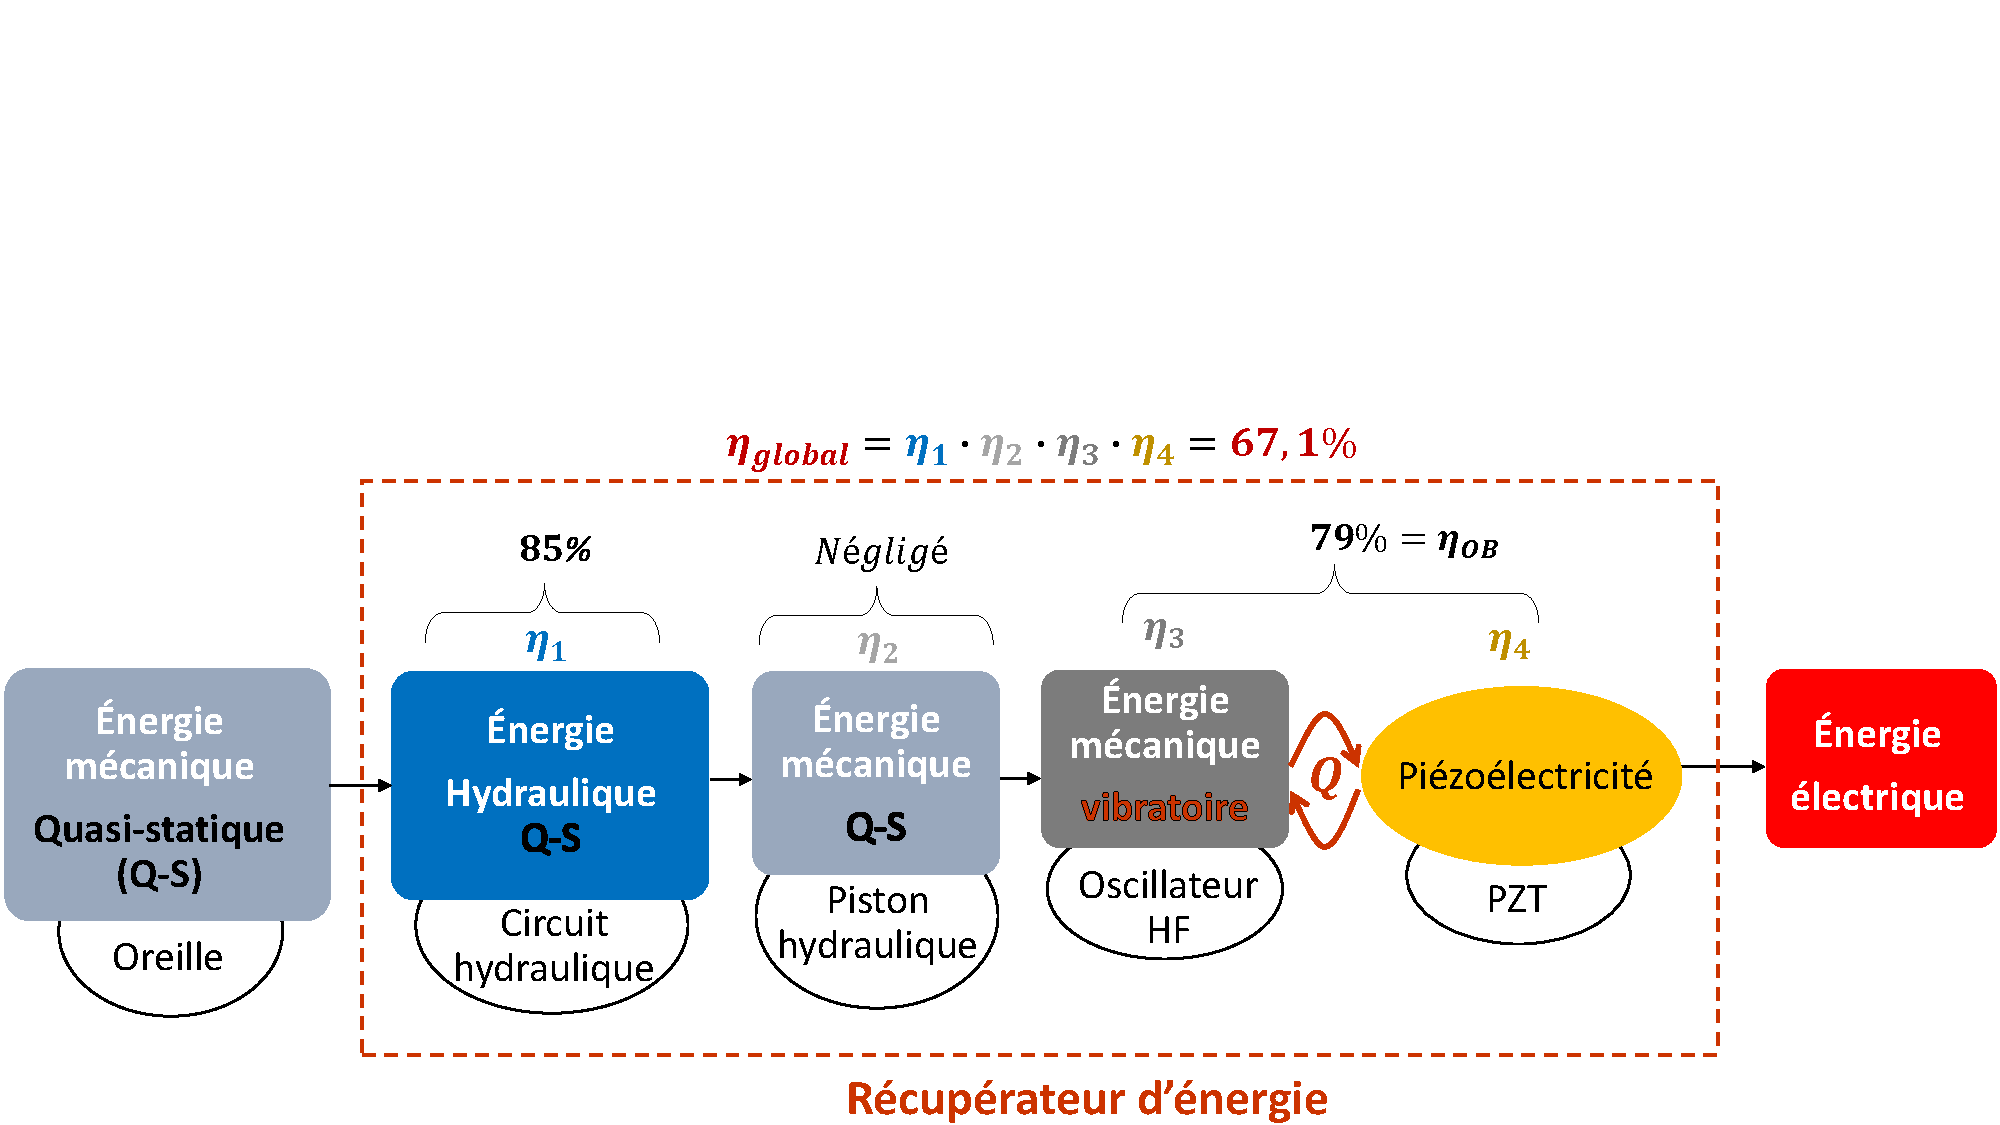
\includegraphics[trim={0cm 0cm 0cm 7cm},clip, width=0.8\textwidth]{figures/conversion_symme_rendements.pdf}
	\caption{$K_{HV}$ impact on the evolution of the BO mass potential energy.}
	\label{fig:conversion_symme_rendements.pdf}
\end{figure*}
%%%%%%%%%%%%%%%%%%%%%%%%%%%%%%%%%%%%%%%
%/!\/!\/!\/!\/!\/!\/!\/!\/!\/!\/!\/!\/!\/!\/!\/!\/!\/!\/!\/!\/!\/!\/!\/!\%
\section{EXPERIMENTAL CHARACTERIZATIONS}
\label{sec:EXPERIMENTAL CHARACTERIZATIONS}
%/!\/!\/!\/!\/!\/!\/!\/!\/!\/!\/!\/!\/!\/!\/!\/!\/!\/!\/!\/!\/!\/!\/!\/!\%
\lipsum[2]
    %///////////////////////////////////////////// 
	\subsection{The electromechanical converter}	
	\label{The electromechanical converter}
    %/////////////////////////////////////////////
%%%%%%%%%%%%%%%%%%%%%%%%%%%%%%%%%%%%%%
\begin{figure*}[!htbp]
\begin{center}
\captionsetup{justification=centering}
	\begin{subfigure} [h!]{0.49\textwidth}
		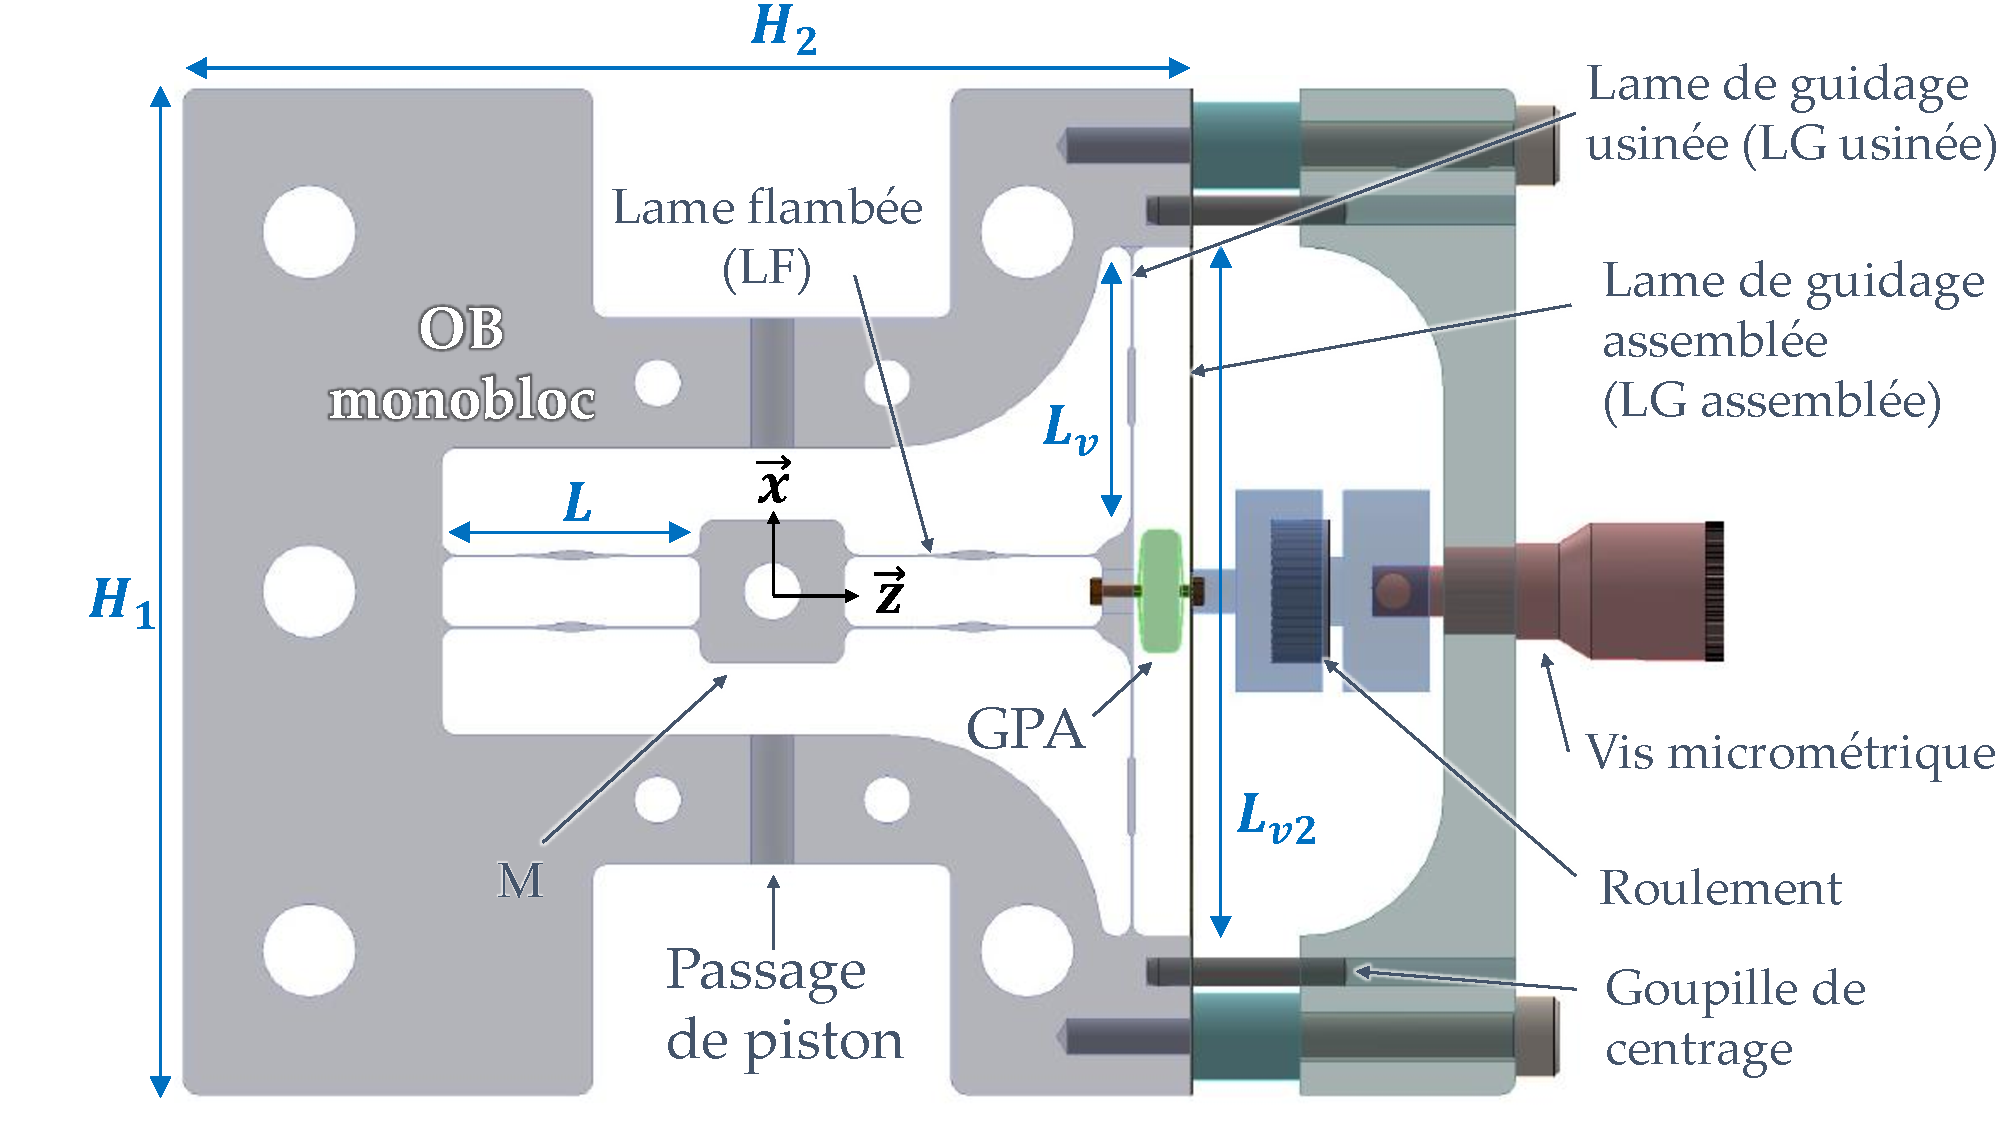
\includegraphics[trim={1.4cm 0cm 0cm 0cm},clip,width=\textwidth]{figures/monobloc+GPA_face.pdf}
		\caption{aaa} 
		\label{fig:/monobloc+GPA_face}
	\end{subfigure}
	%\hfill
	\begin{subfigure}[h!]{0.49\textwidth}
		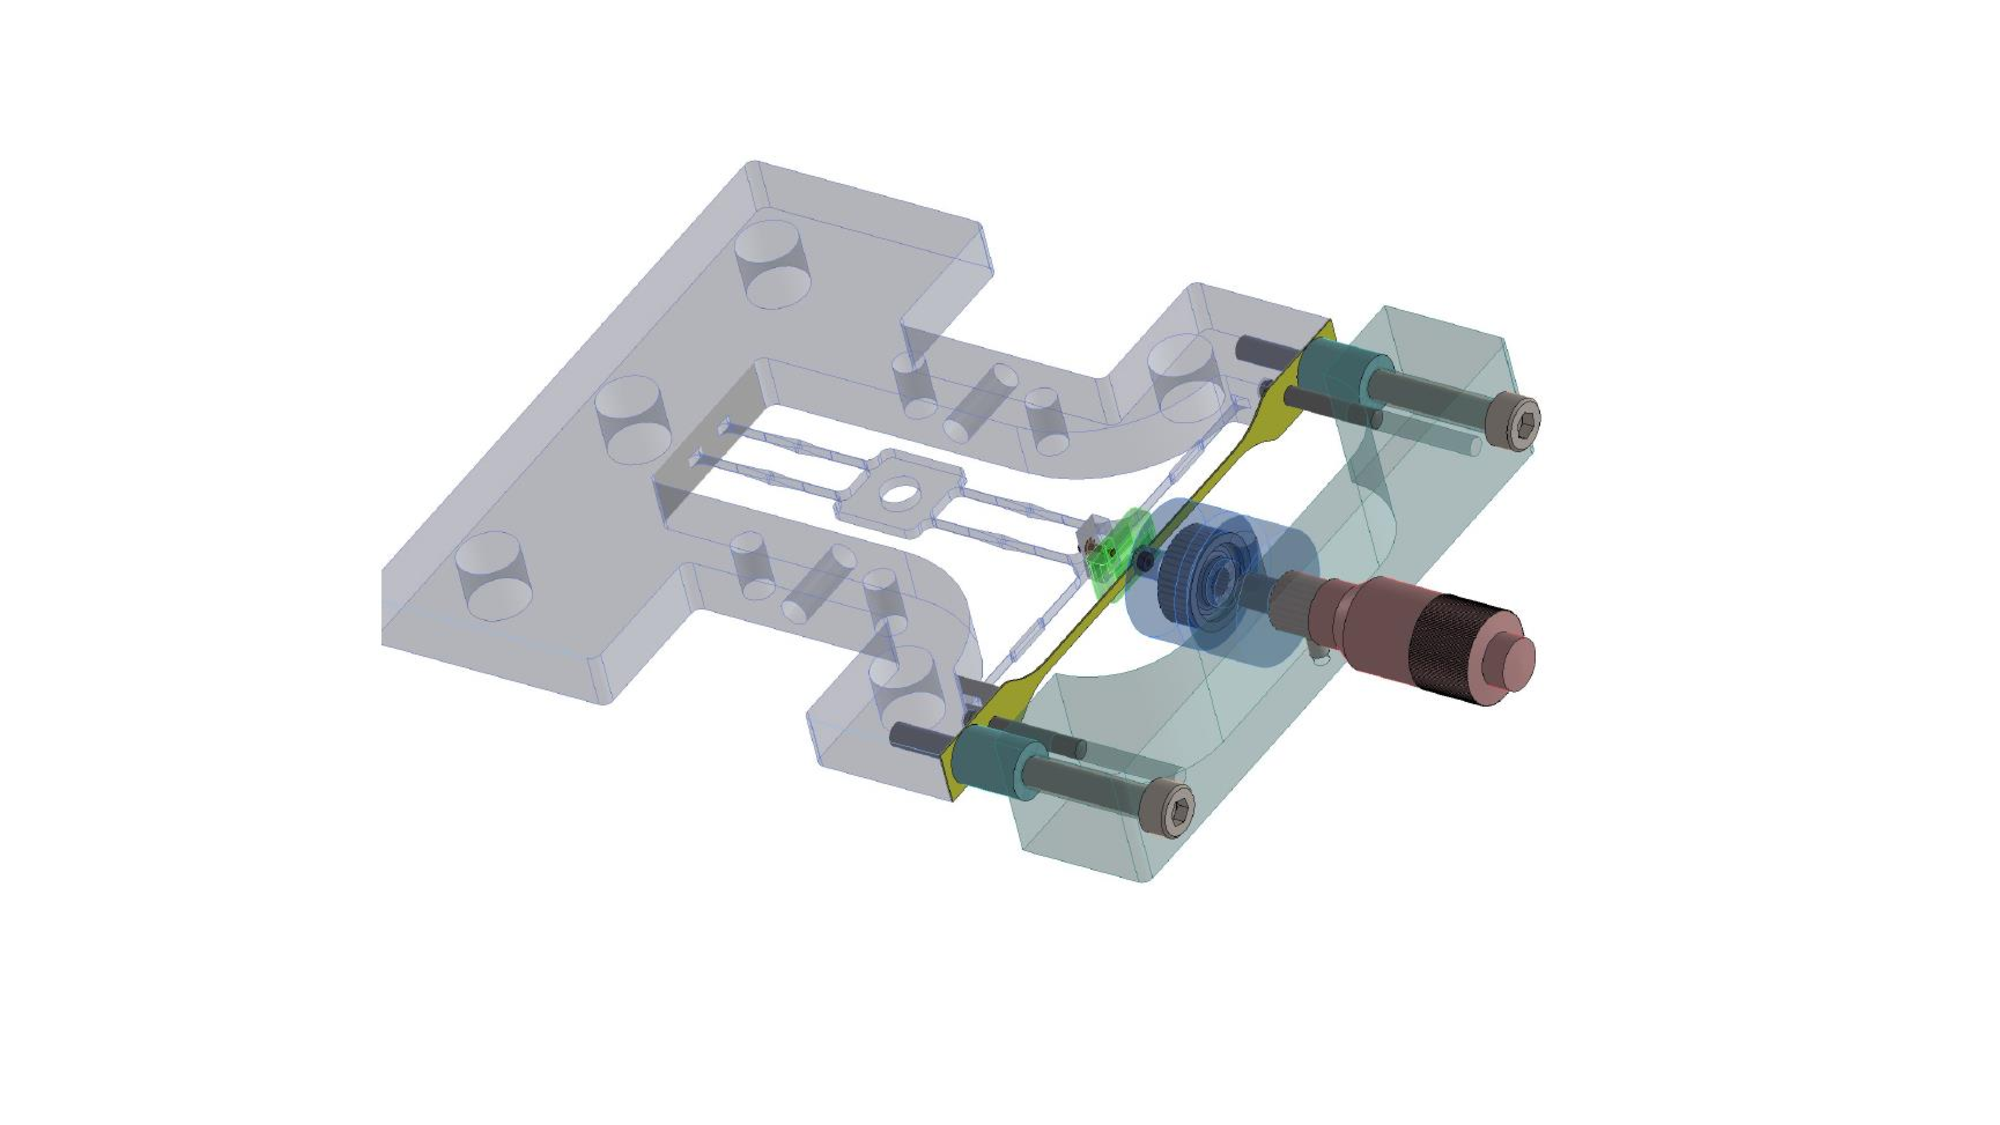
\includegraphics[trim={6cm 3cm 7.5cm 2.6cm},clip, width=\textwidth]{figures/monobloc+GPA_iso.pdf}
		\caption{aaa}  
		\label{fig:/monobloc+GPA_iso}
	\end{subfigure}
	\caption{aaa}
\end{center}
\label{fig:/monobloc+GPA_face}
\end{figure*}
%%%%%%%%%%%%%%%%%%%%%%%%%%%%%%%%%%%%%%
\lipsum[1]
%%%%%%%%%%%%%%%%%%%%%%%%%%%%%%%%%%%%%%
\begin{figure}[!htbp]
	\centering
	\captionsetup{justification=centering}
	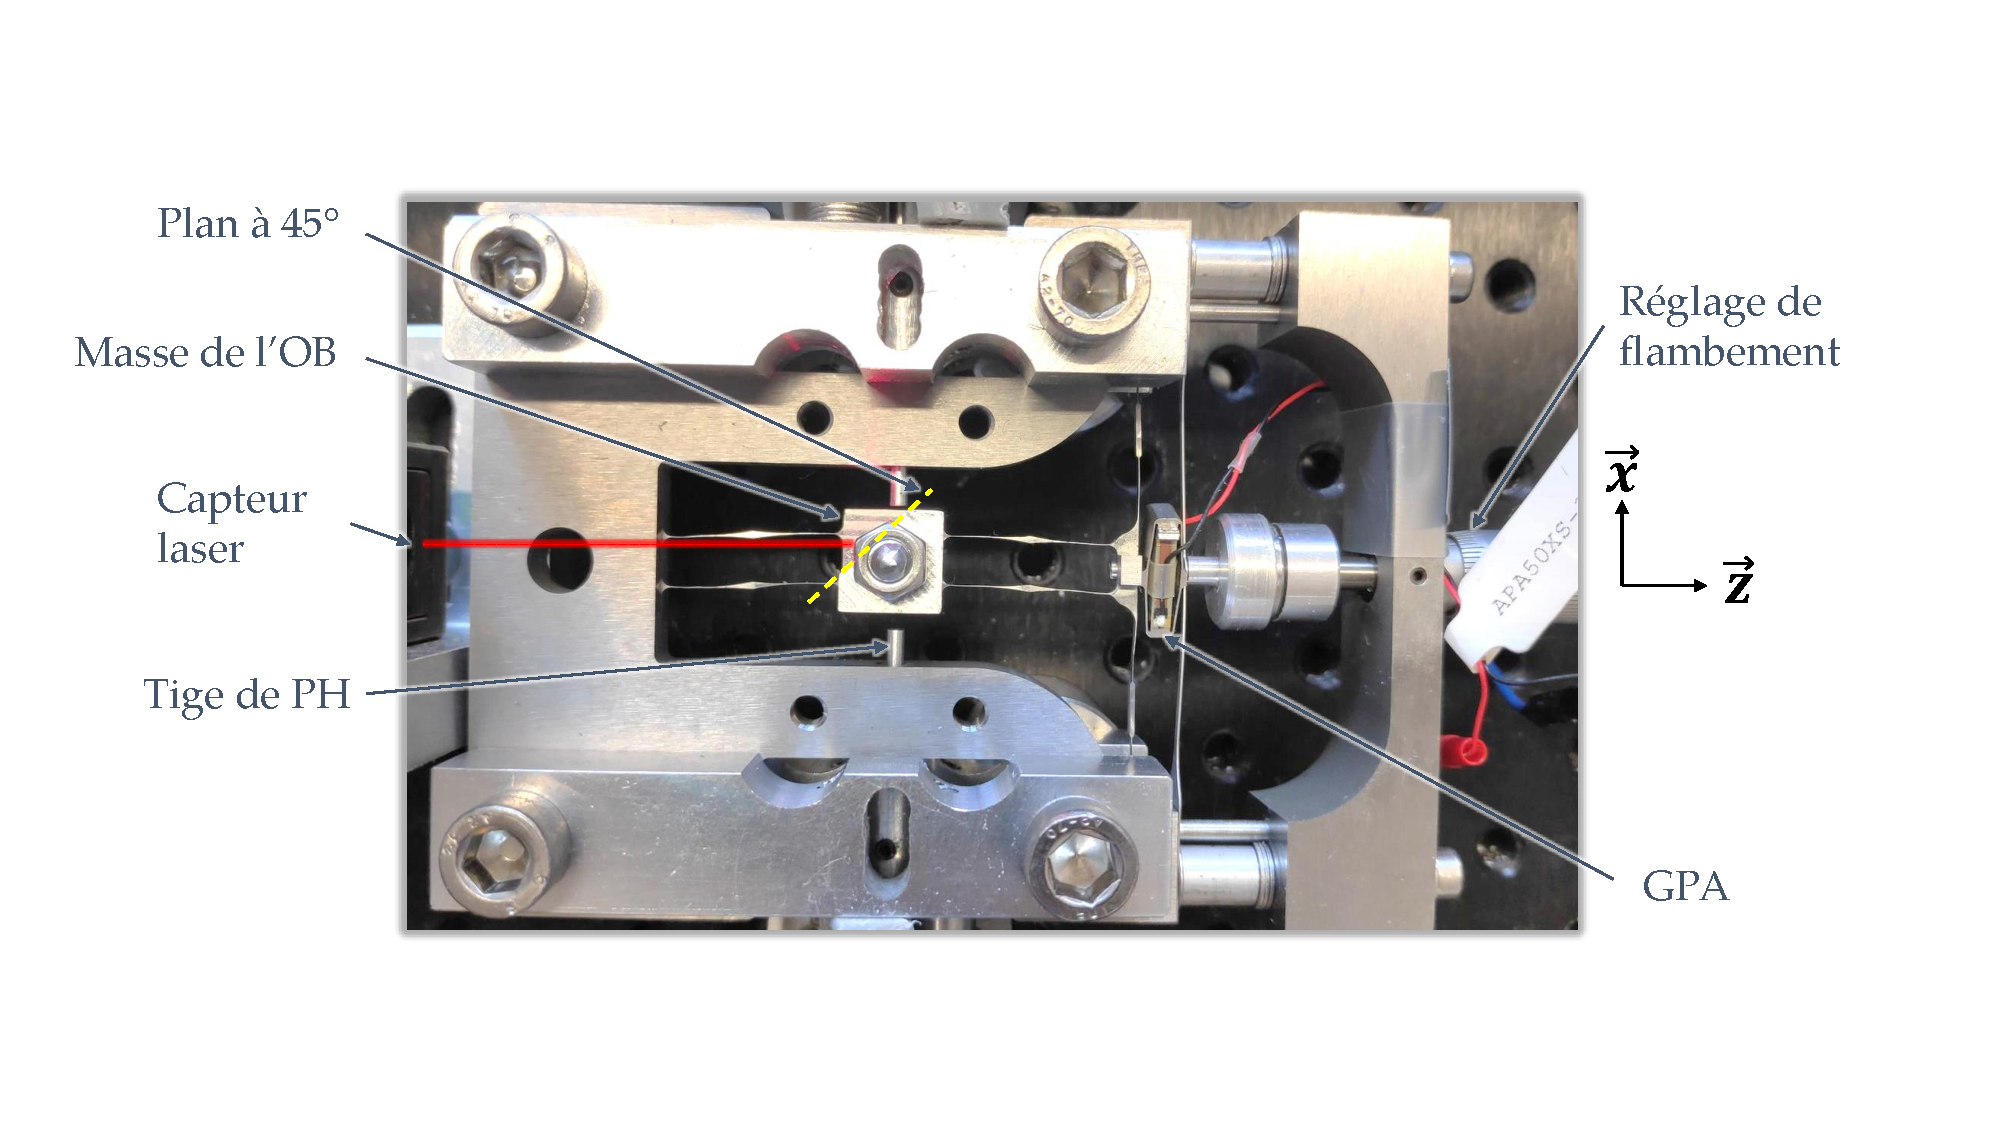
\includegraphics[trim={1cm 3cm 2cm 2.5cm},clip,width=0.45\textwidth]{figures/BDT_OB+GPA.pdf}
	\caption{Vue de face de GPA et l’OB monobloc sur le banc de caractérisation
	électromécanique.}
	\label{fig:BDT_OB+GPA}
\end{figure}
%%%%%%%%%%%%%%%%%%%%%%%%%%%%%%%%%%%%%%%
%%%%%%%%%%%%%%%%%
\begin{table*}[!htbp]
\centering
	\begin{tabular}{ l | c | c }
		\toprule
		\multicolumn{1}{c}{\textbf{Symbole}}  &
		\multicolumn{1}{c}{\textbf{Simulation avec paramètres théoriques}}  &
		\multicolumn{1}{c}{\textbf{Simulation avec paramètres expérimentaux}} \\
		\midrule
		$Q$                       & 50.0                  & 30.0 		  	\\  
		$f_0$                     & 47.0 Hz               & 27.9 Hz  		\\
		$x_0$                     & 0.49 mm               & 0.50 mm    		\\
		$K$                       & 2.56e5 N/m            & 0.85e5 N/m 		\\
		${k^2_{sys}}$             & 8.72 \%               & 1.25 \% 		\\
		$\eta_{ob}$               & 79 \%                 & 12.9 \%   		\\
		\bottomrule
	\end{tabular}
	\caption{Valeur des paramètres de l'OB issus du test de lâcher expérimental, comparés aux valeurs théoriques}
\label{tab:parametres_lacher_free}
\end{table*} 
%%%%%%%%%%%%%%%%%%%%%  
    %///////////////////////////////////////////// 
	\subsection{The hydraulic valves}	
	\label{The hydraulic valves}
    %/////////////////////////////////////////////
    		%************* 
			\subsubsection{Static characterizations}
			\label{Static characterizations of HV}
    		%************* 
	%%%%%%%%%%%%%%%%%%%%%%%%%%%%%%%%%%%%	
\begin{figure*}[!htb]
	\begin{center}
		\begin{subfigure}[t]{0.69\textwidth}
			\captionsetup{justification=centering}
			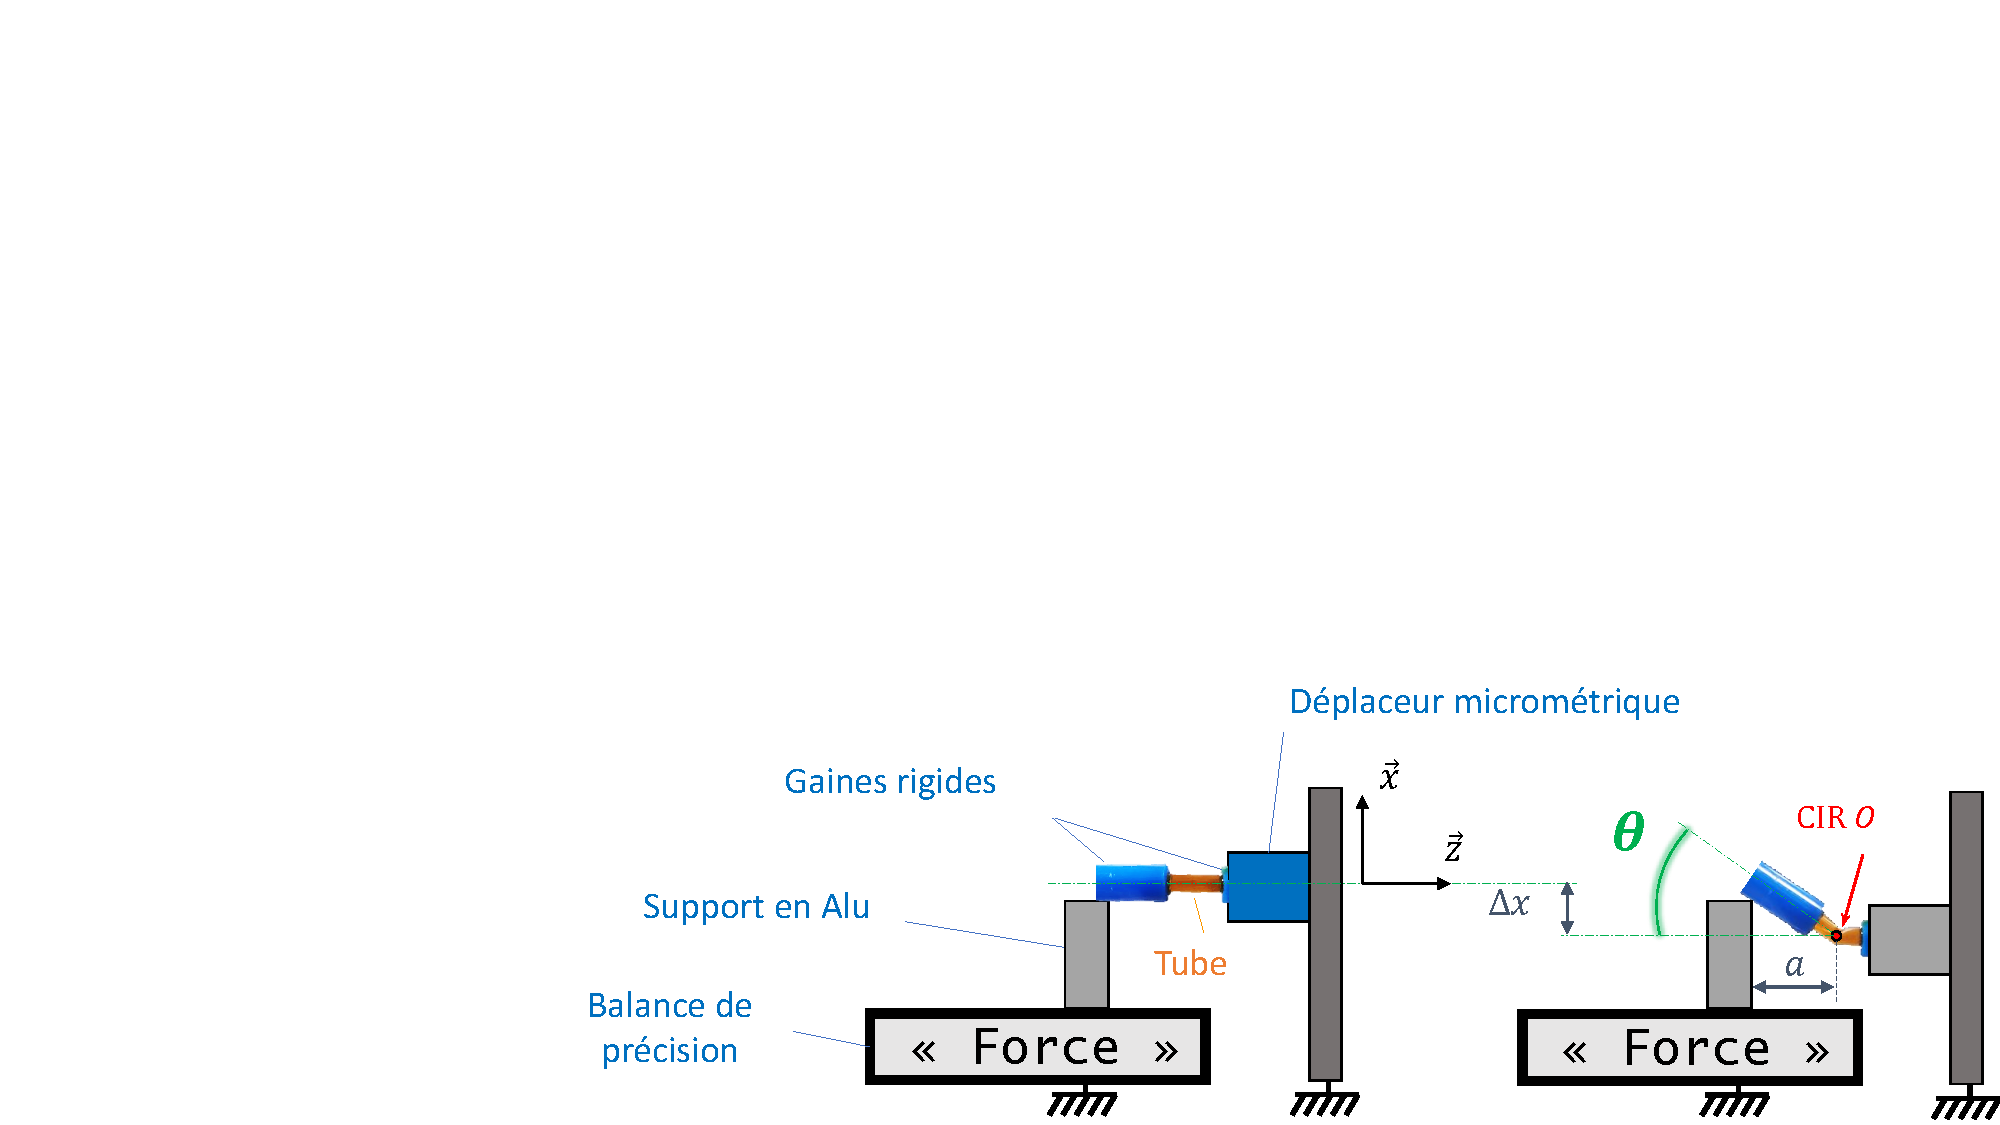
\includegraphics[trim={9.8cm 0cm 0cm 11cm},clip,width=\textwidth]{figures/essais_statique_VH.pdf}
			\caption{Vue globale}
			\label{fig:essais_statique_VH}
		\end{subfigure}
		\hfillx
		\begin{subfigure}[t]{0.29\textwidth}
			\captionsetup{justification=centering}
			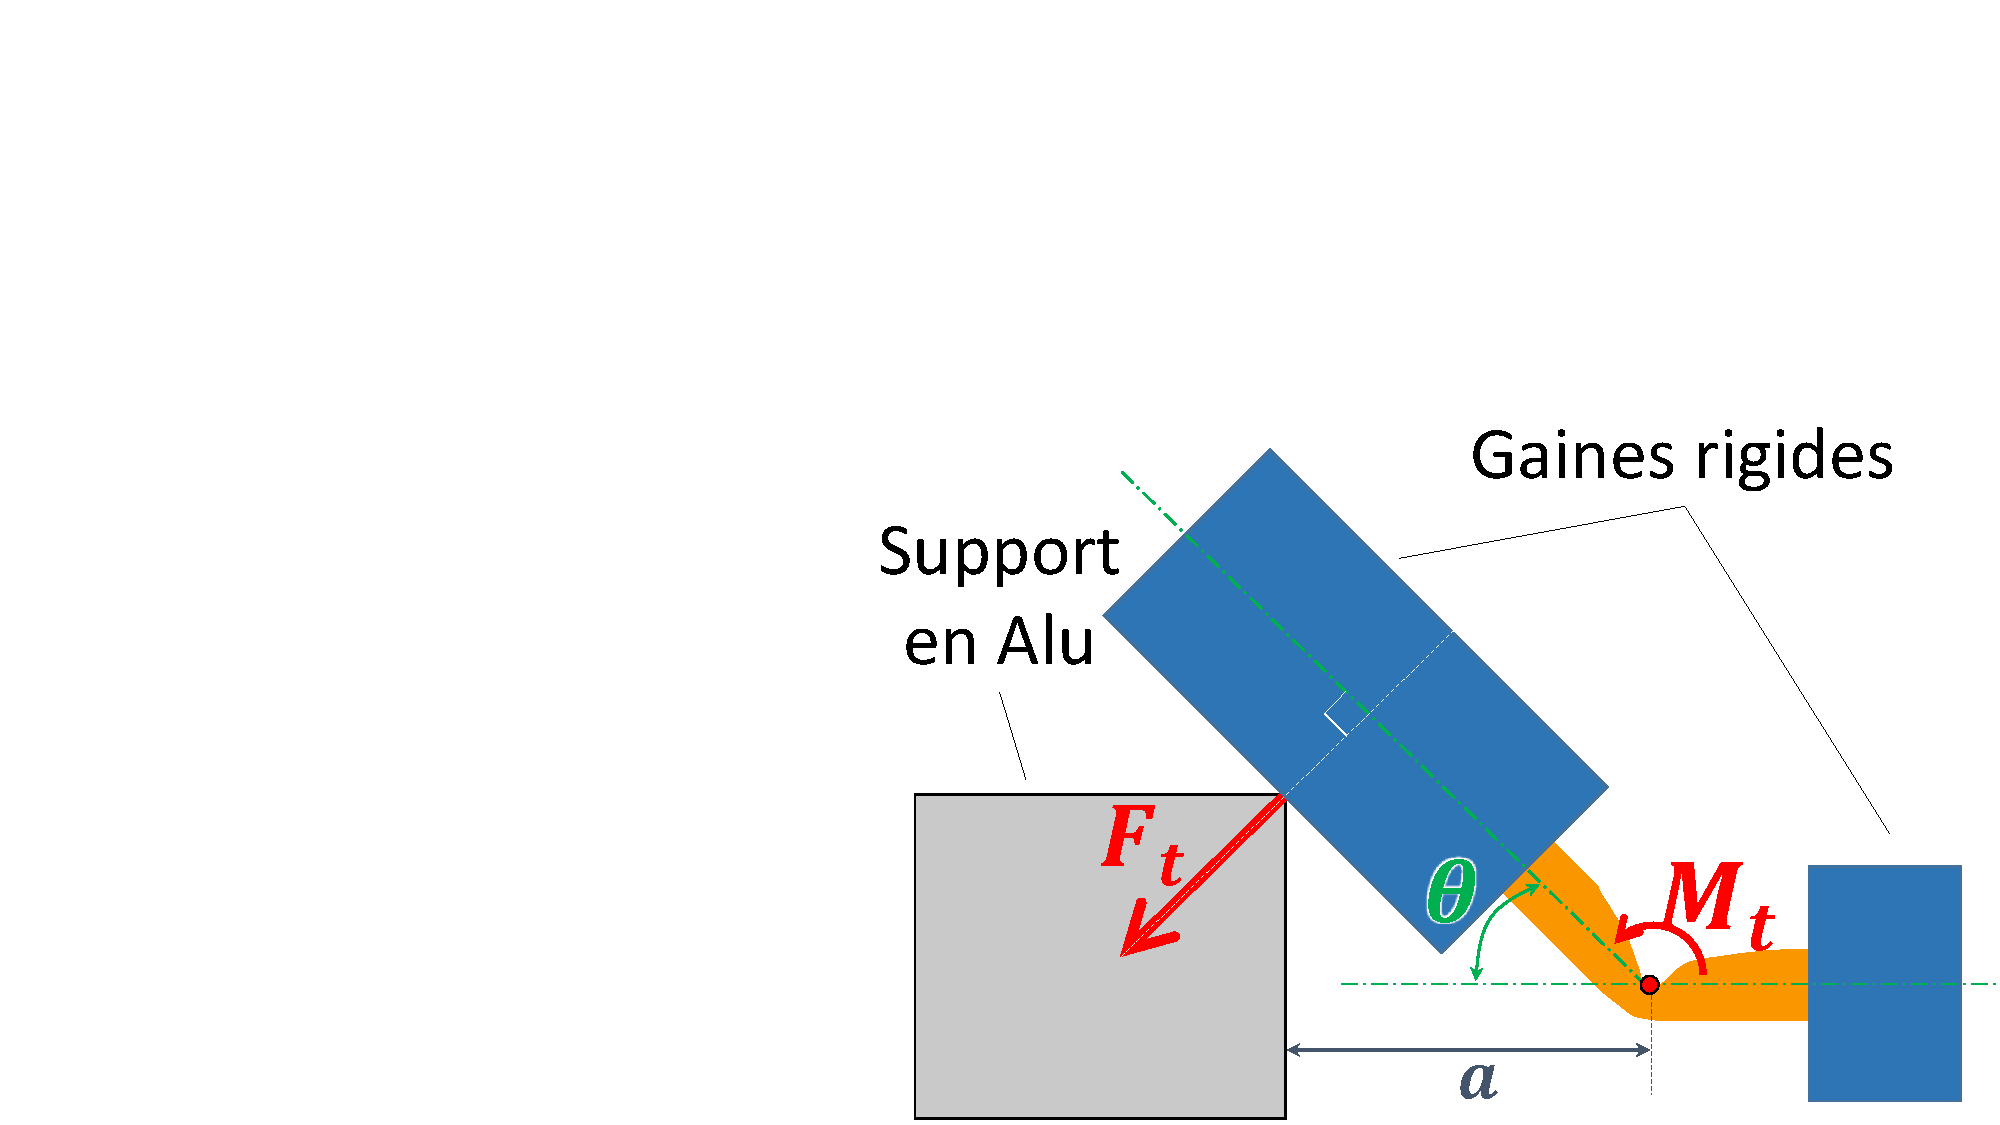
\includegraphics[trim={14cm 0cm 0cm 7cm},clip,width=\textwidth]{figures/essais_statique_detail.pdf}
			\caption{Détail du contact support-échantillon}
			\label{fig:essais_statique_detail}
		\end{subfigure}
		\caption{Schéma des essais de caractérisations statiques de tubes en flexion}
		\label{fig:essais_statique_total}
	\end{center}
\end{figure*}
%%%%%%%%%%%%%%%%%%%%%%%%%%%%%%%%%%%% 
%%%%%%%%%%%%%%%%%%%%%%%%%%%%%%%%%%%%	
\begin{figure*}[!htb]
	\begin{center}
		\captionsetup{justification=centering}
		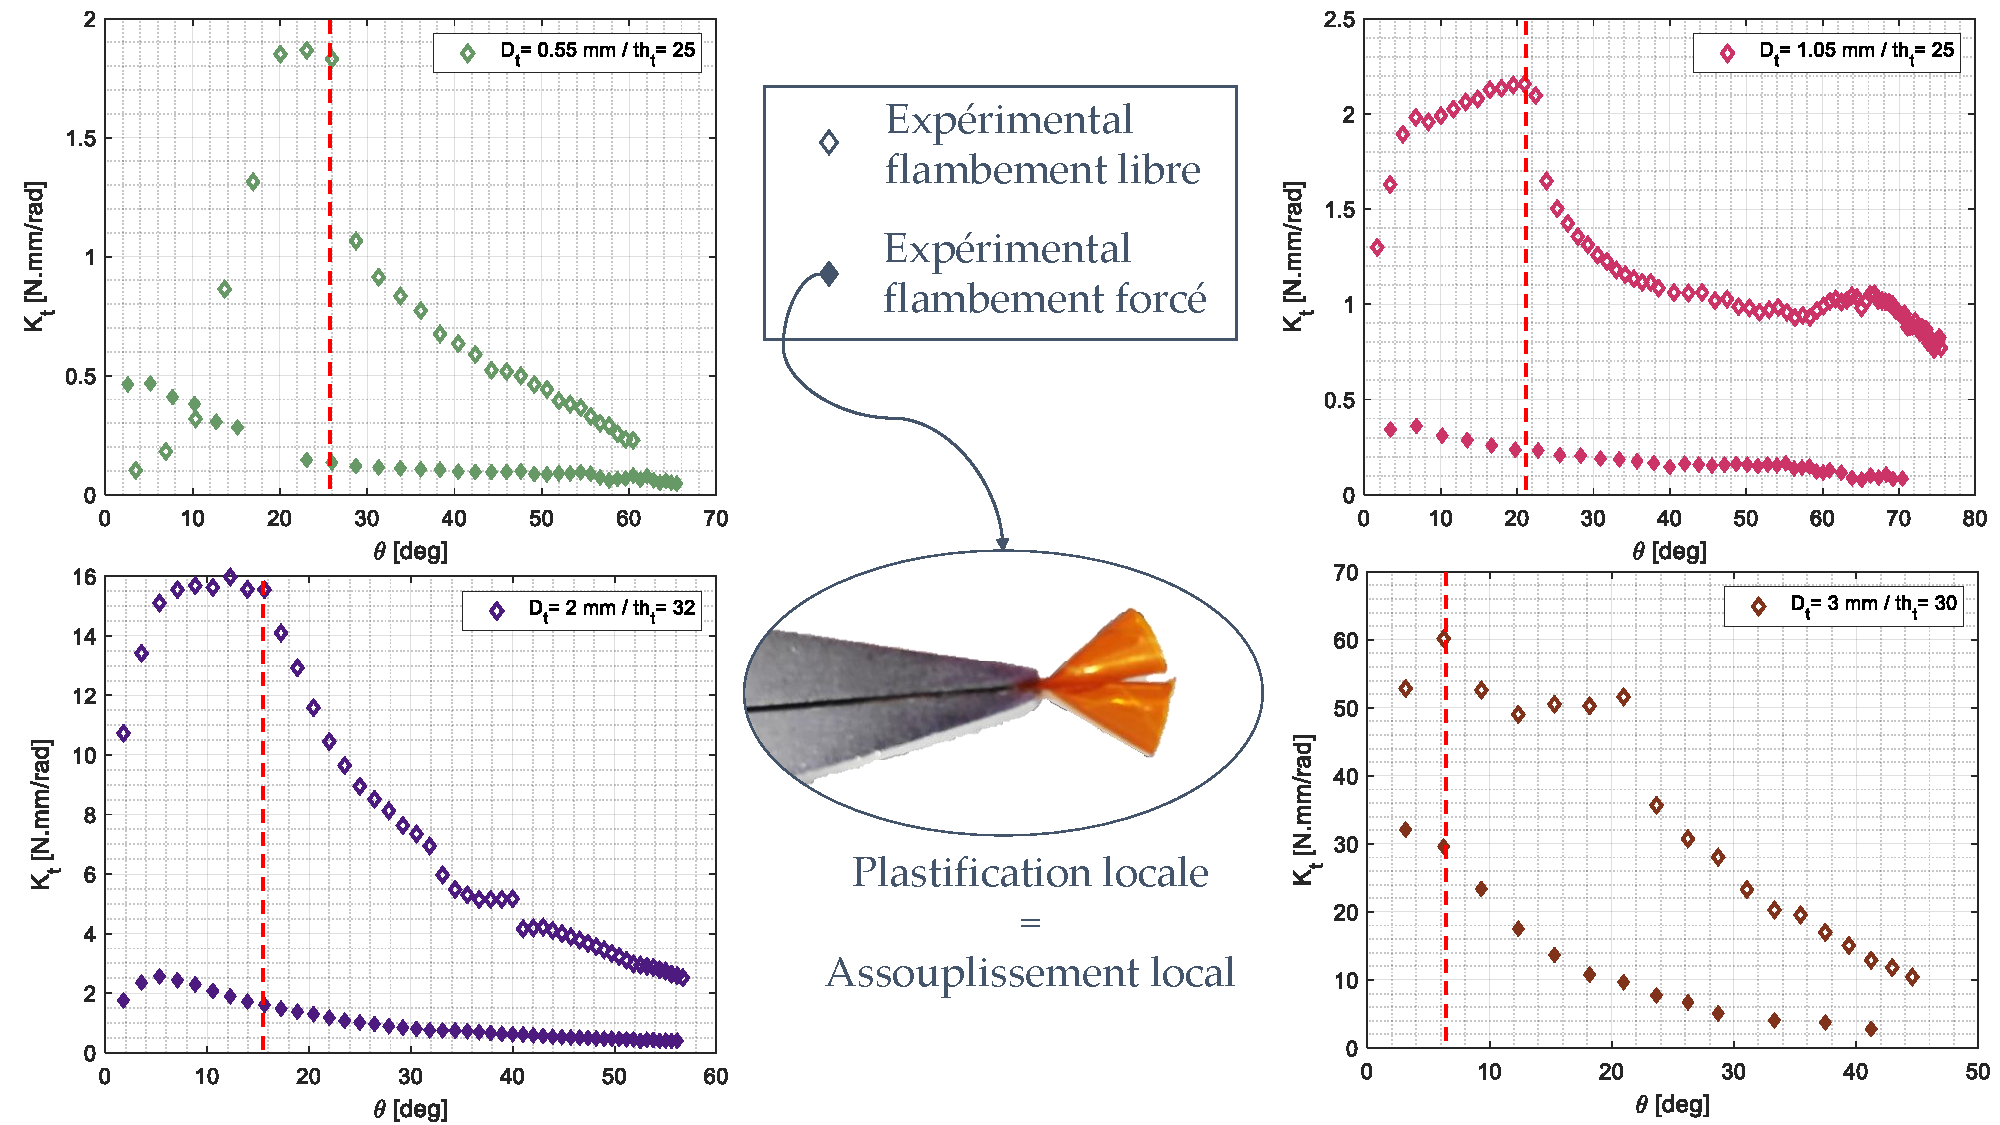
\includegraphics[trim={0cm 0cm 0cm 0cm},clip,width=\textwidth]{figures/resultats_essais_statique_VH_tous_sans_simu.pdf}
		\caption{Évolutions expérimentales de $K_t$ en fonction de $\theta$ pour quatre tubes de dimensions différentes (tab. \ref{tab:dim_tube_statique})}
		\label{fig:resultats_essais_statique_VH_tous}
	\end{center}
\end{figure*} 
%%%%%%%%%%%%%%%%%%%%%%%%%%%%%%%%%%%% 
    		%************* 
			\subsubsection{Hydraulic characterizations}
			\label{Hydraulic characterizations}
    		%************* 
%%%%%%%%%%%%%%%%%%%%%%%%%%%%%%%%%%%%	
\begin{figure*}[!htb]
\begin{center}
	\captionsetup{justification=centering} 
	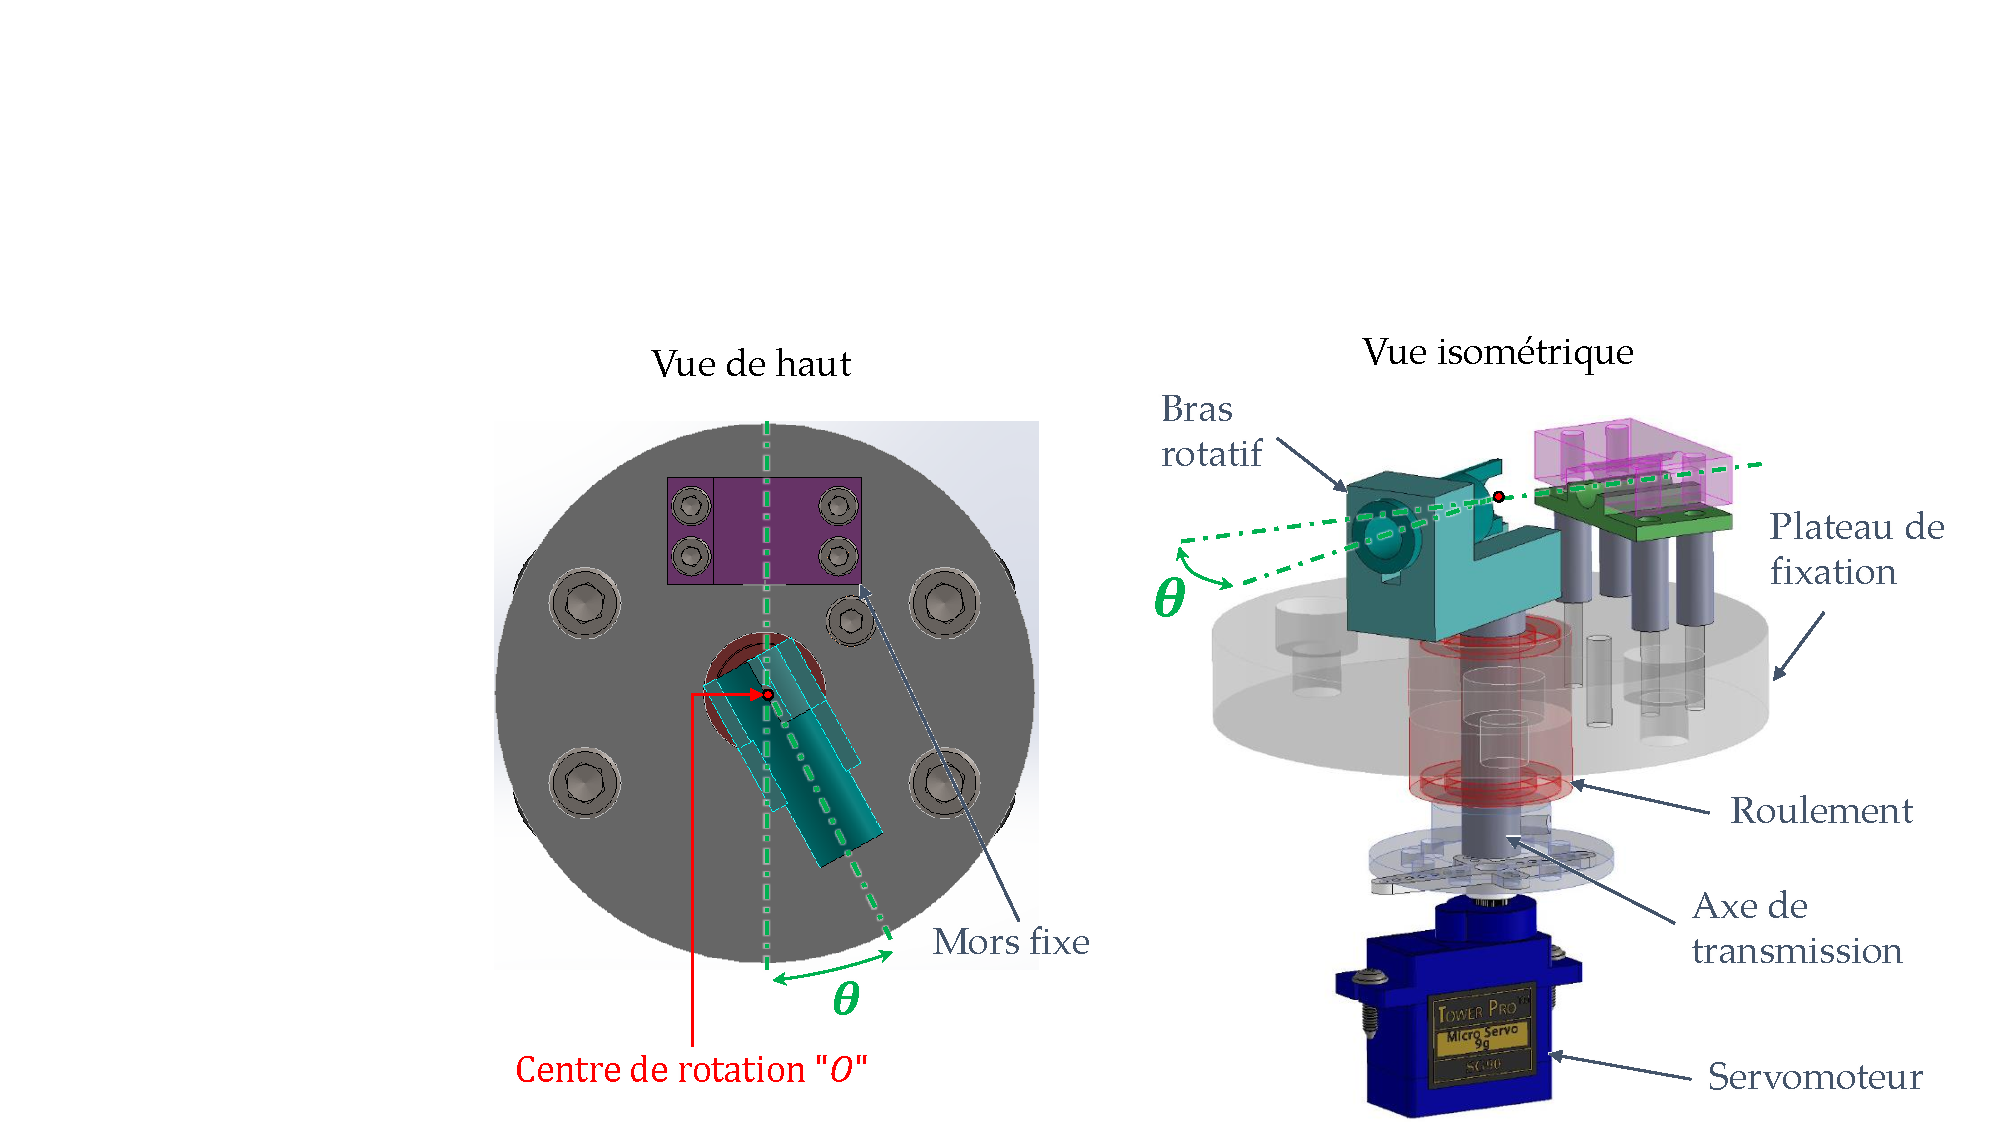
\includegraphics[trim={8cm 0cm 0cm 5cm},clip,width=0.8\textwidth]{figures/BDT_hydraulique_VH.pdf}
	\caption{Banc d'essai pour la caractérisations hydrauliques de VH}
	\label{fig:BDT_hydraulique_VH}
\end{center}	
\end{figure*}    
%%%%%%%%%%%%%%%%%%%%%%%%%%%%%%%%%%%% 
%%%%%%%%%%%%%%%%%%%%%%%%%%%%%%%%%%%%	
\begin{figure*}[!htb]
\begin{center}
	\captionsetup{justification=centering} 
	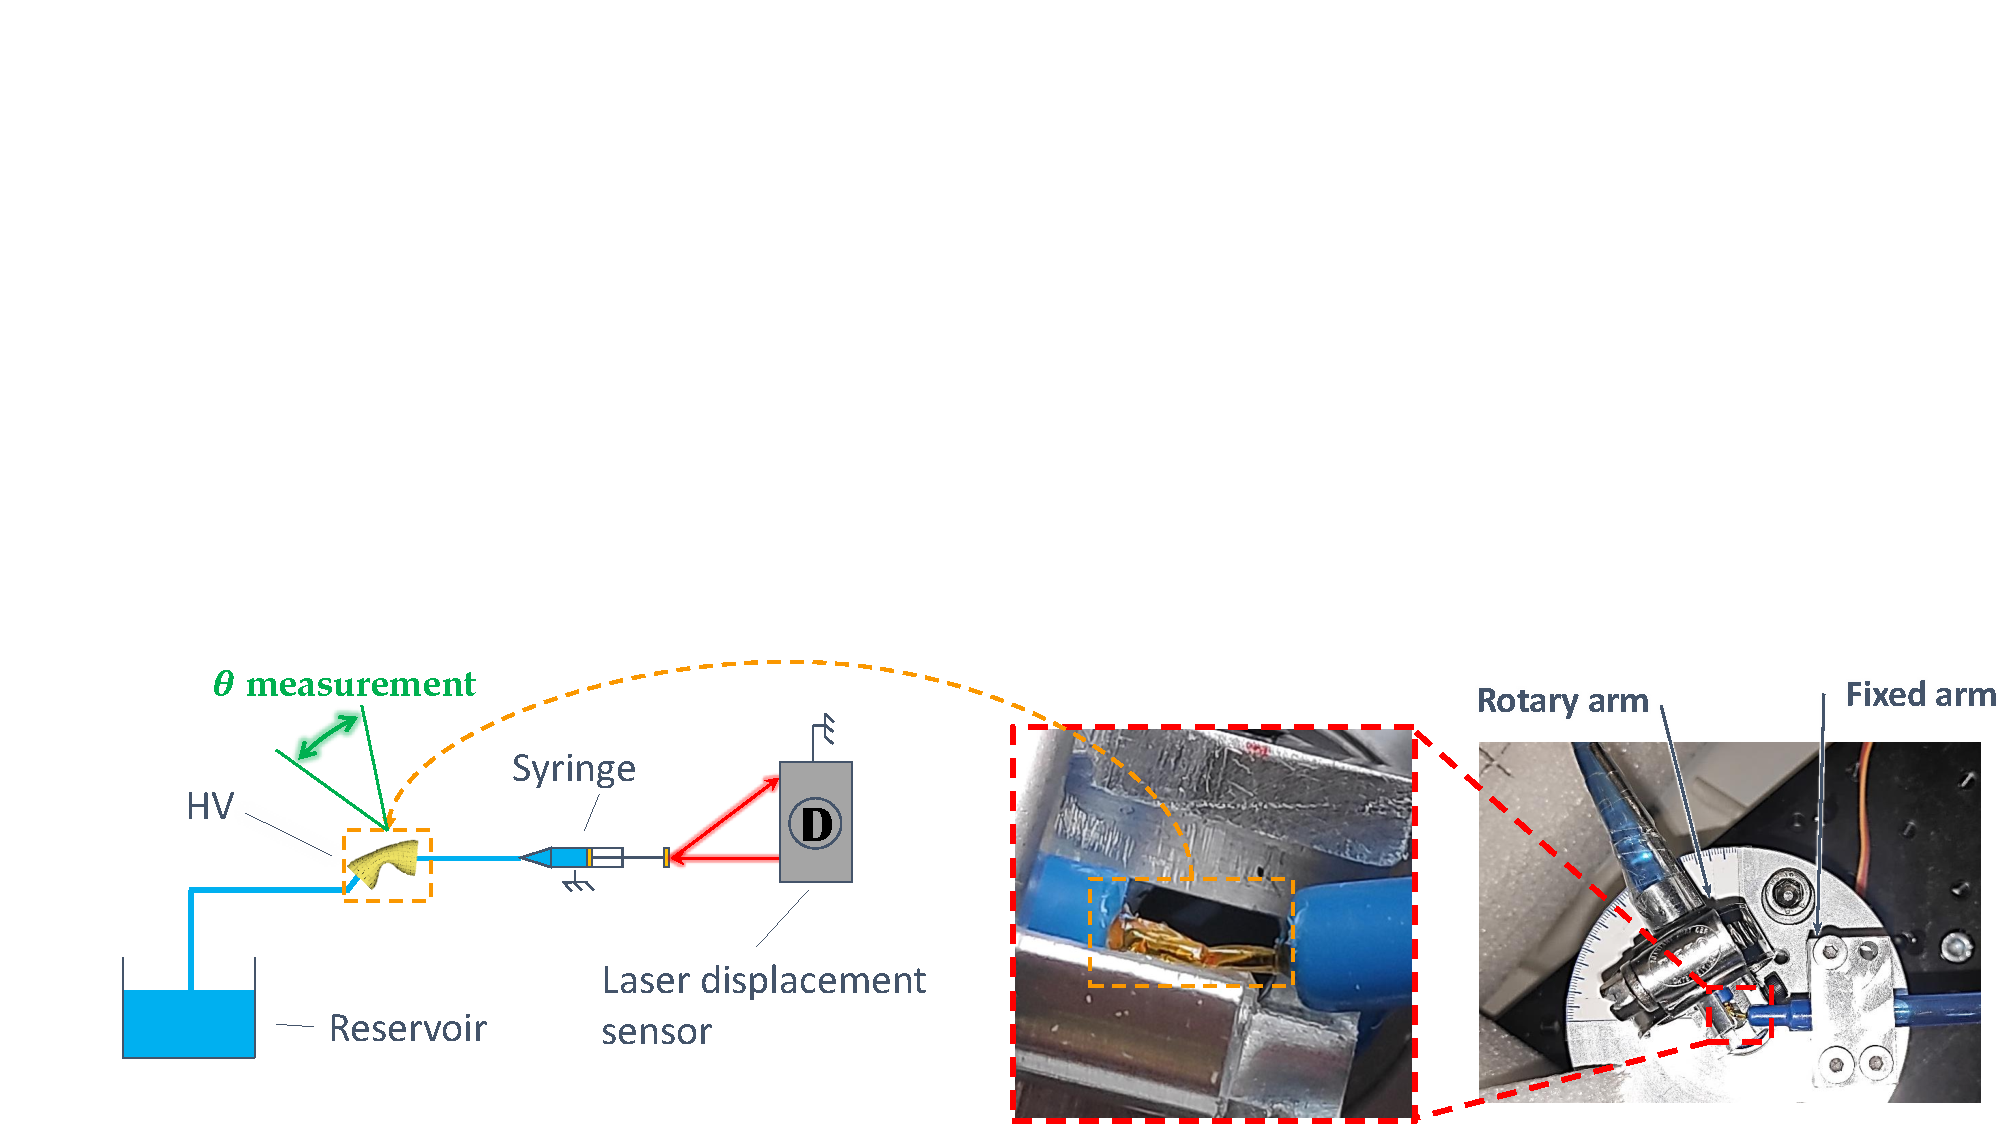
\includegraphics[trim={2cm 0cm 0cm 10cm},clip,width=\textwidth]{figures/essais_hydraulique_VH.pdf}
	\caption{Essais de caractérisations hydrauliques de VH}
	\label{fig:essais_hydraulique_VH}
\end{center}	
\end{figure*}    
%%%%%%%%%%%%%%%%%%%%%%%%%%%%%%%%%%%%  
%%%%%%%%%%%%%%%%%%%%%%%%%%%%%%%%%%%%	
\begin{figure}[!htb]
\begin{center}
	\captionsetup{justification=centering} 
	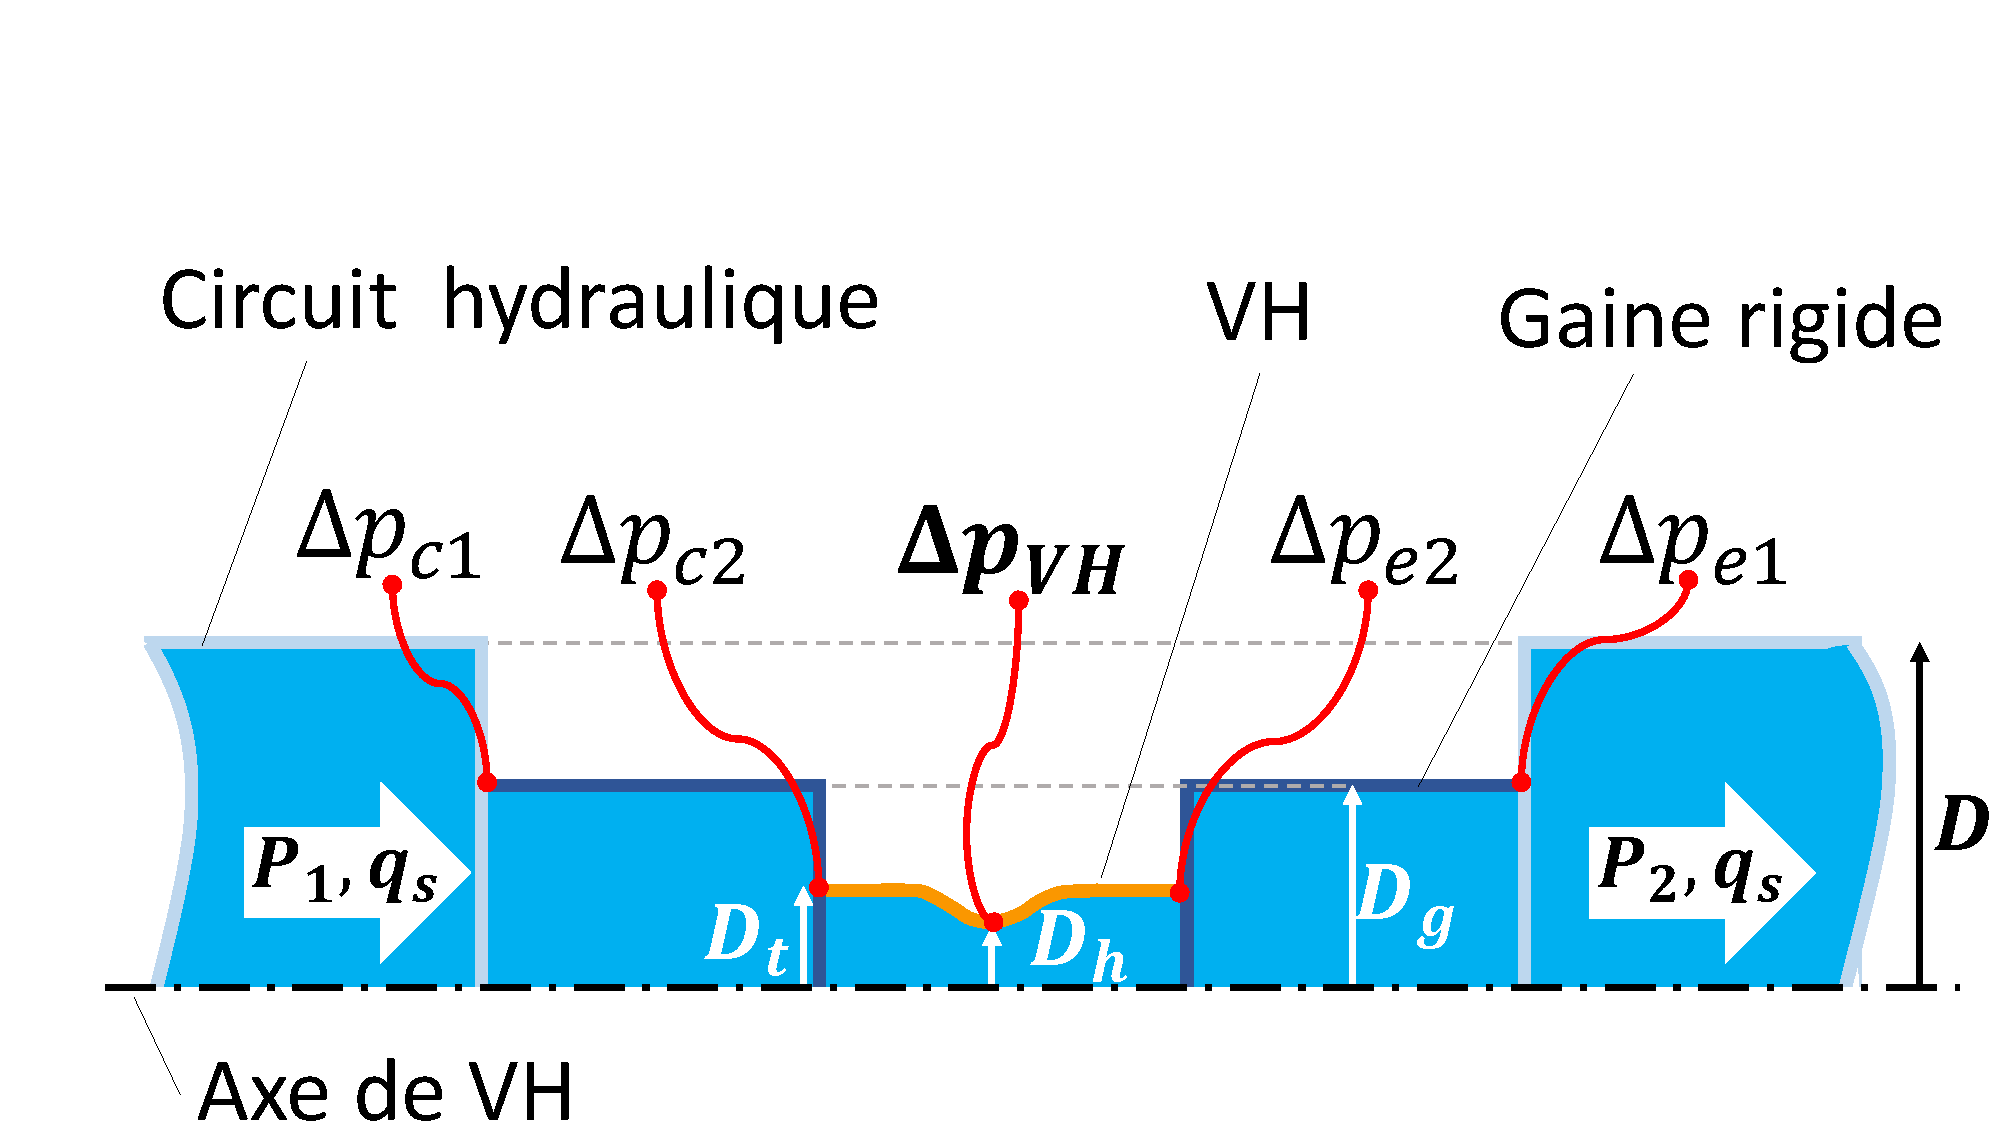
\includegraphics[trim={2cm 0cm 0cm 4cm},clip,width=0.49\textwidth]{figures/fabrication_tube_experimental.pdf}
	\caption{Méthode de fabrication de la VH}
	\label{fig:fabrication_tube_experimental}
\end{center}	
\end{figure}    
%%%%%%%%%%%%%%%%%%%%%%%%%%%%%%%%%%%% 
%%%%%%%%%%%%%%%%%%%%%%%%%
\begin{figure}[!htbp]
\begin{center}
	\captionsetup{justification=centering}
	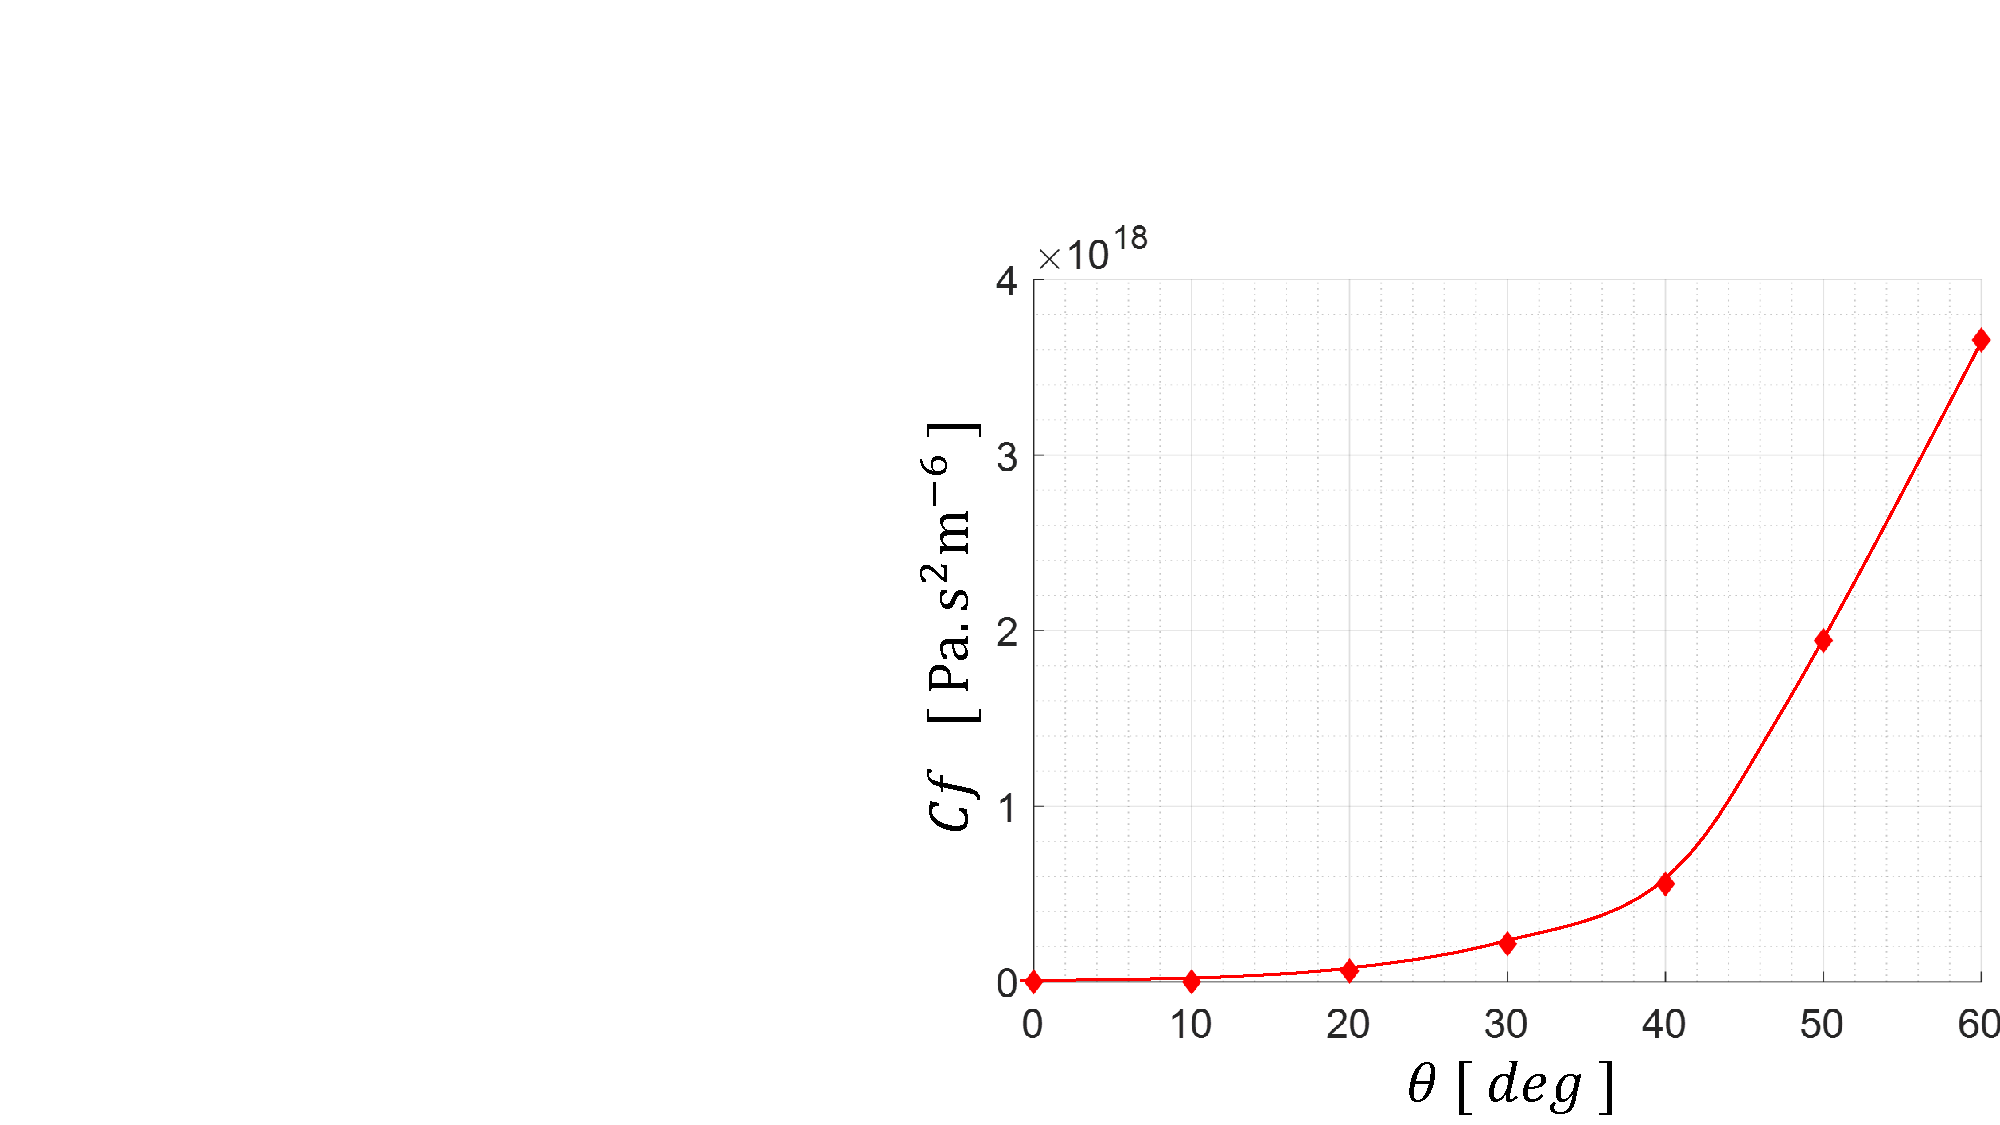
\includegraphics[trim={10cm 0cm 0cm 0cm},clip,width=0.49\textwidth]{figures/resultats_essais_hydraulique_VH_D1mm.pdf}
	\caption{$Cf_{VH}$ calculé à partir des essais pour 7 incréments d'angles}
	\label{fig:resultats_essais_hydraulique_VH_D1mm}
\end{center}
\end{figure}
%%%%%%%%%%%%%%%%
	%/////////////////////////////////////////////
	\subsection{The valve mechanical influence on the electromechanical converter}	
	\label{The mechanical influence of the valve on the electromechanical converter}
	%/////////////////////////////////////////////
%%%%%%%%%%%%%%%%%%%%%%%%%%%%%%%%%
\begin{figure*}[!htbp]
\begin{center}
	\begin{subfigure}[b]{0.49\textwidth}
	\captionsetup{justification=centering} 
	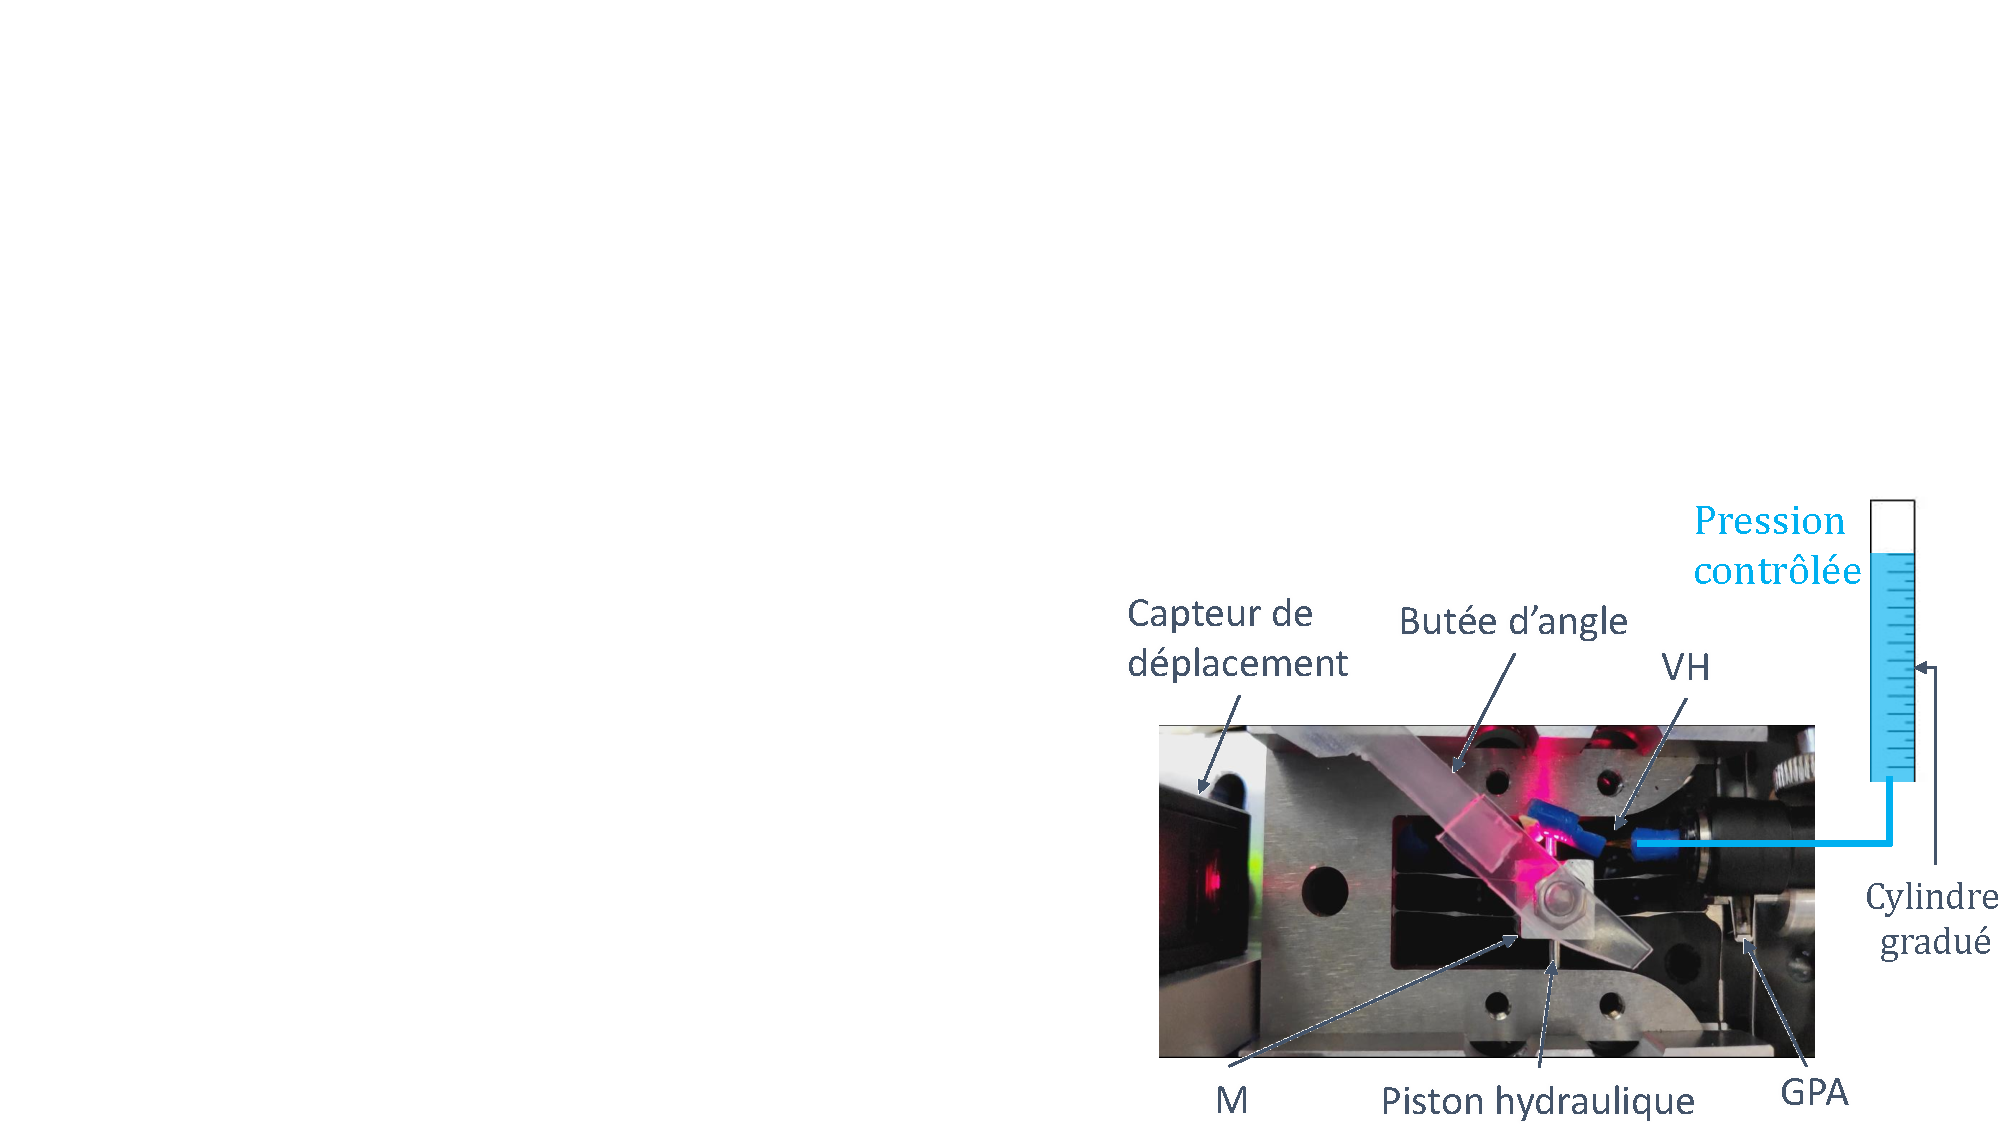
\includegraphics[trim={19cm 0cm 0cm 8cm},clip,width=\textwidth]{figures/presentation_BDT_avant_actionnement.pdf}
	\caption{Avant lâcher : $x_m=-x_0$}
	\label{fig:presentation_BDT_lacher_avant_actionnement}
	\end{subfigure}
\hfillx
	\begin{subfigure}[b]{0.49\textwidth}
	\captionsetup{justification=centering} 
	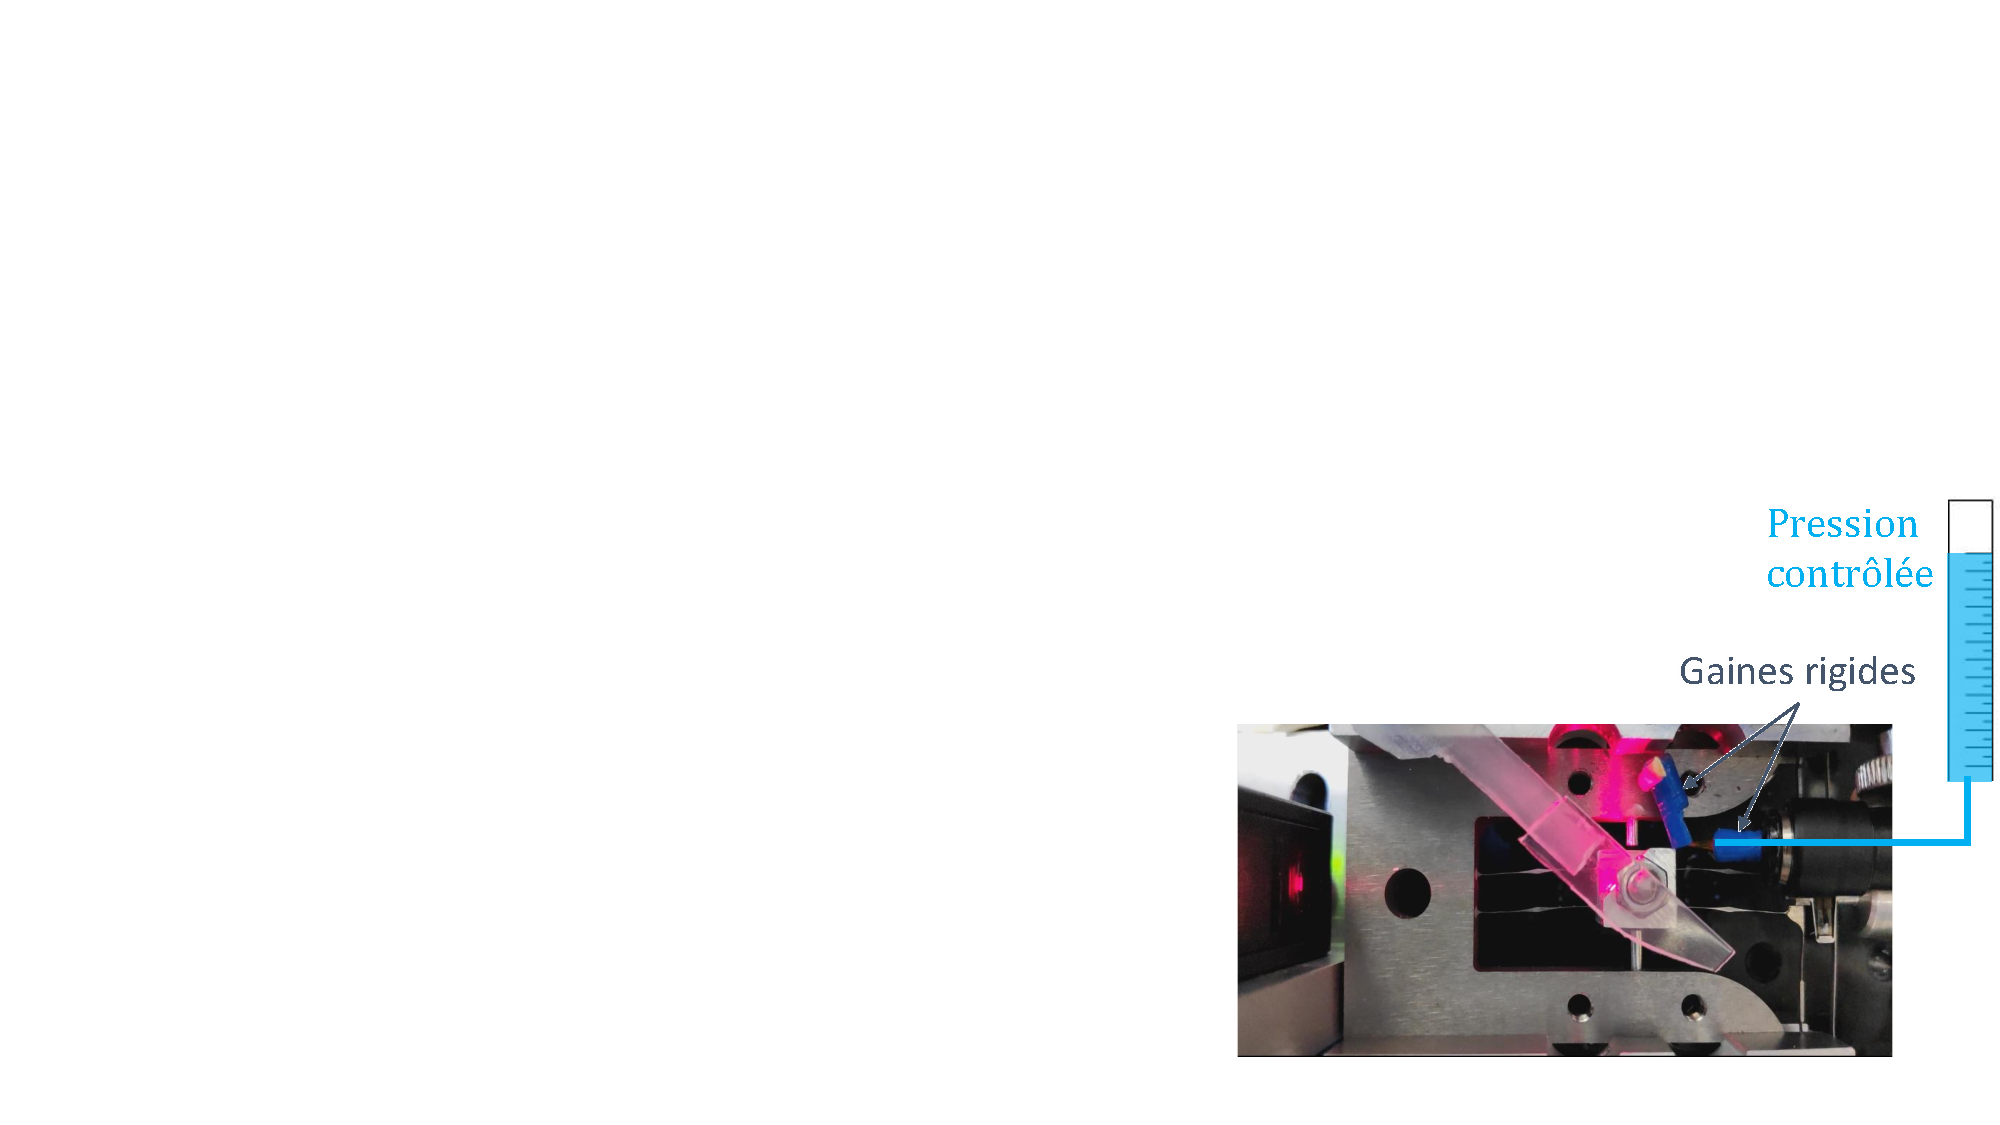
\includegraphics[trim={19cm 0cm 0cm 8cm},clip,width=\textwidth]{figures/presentation_BDT_apres_actionnement.pdf}
	\caption{Après lâcher : $x_m=x_{0,vh}$}
	\label{fig:presentation_BDT_lacher_apres_actionnement}
	\end{subfigure}
	\caption{Présentation du banc de test de lâcher avec VH}
	\label{fig:presentation_BDT_lacher_tube}
\end{center}	
\end{figure*} 
%%%%%%%%%%%%%%%%%%%%%%%%%%%%%%%%%
%%%%%%%%%%%%%%%%%%%%%%%%%%%%%%%%%%%%	
\begin{figure}[!htbp]
\begin{center}
	\captionsetup{justification=centering}
	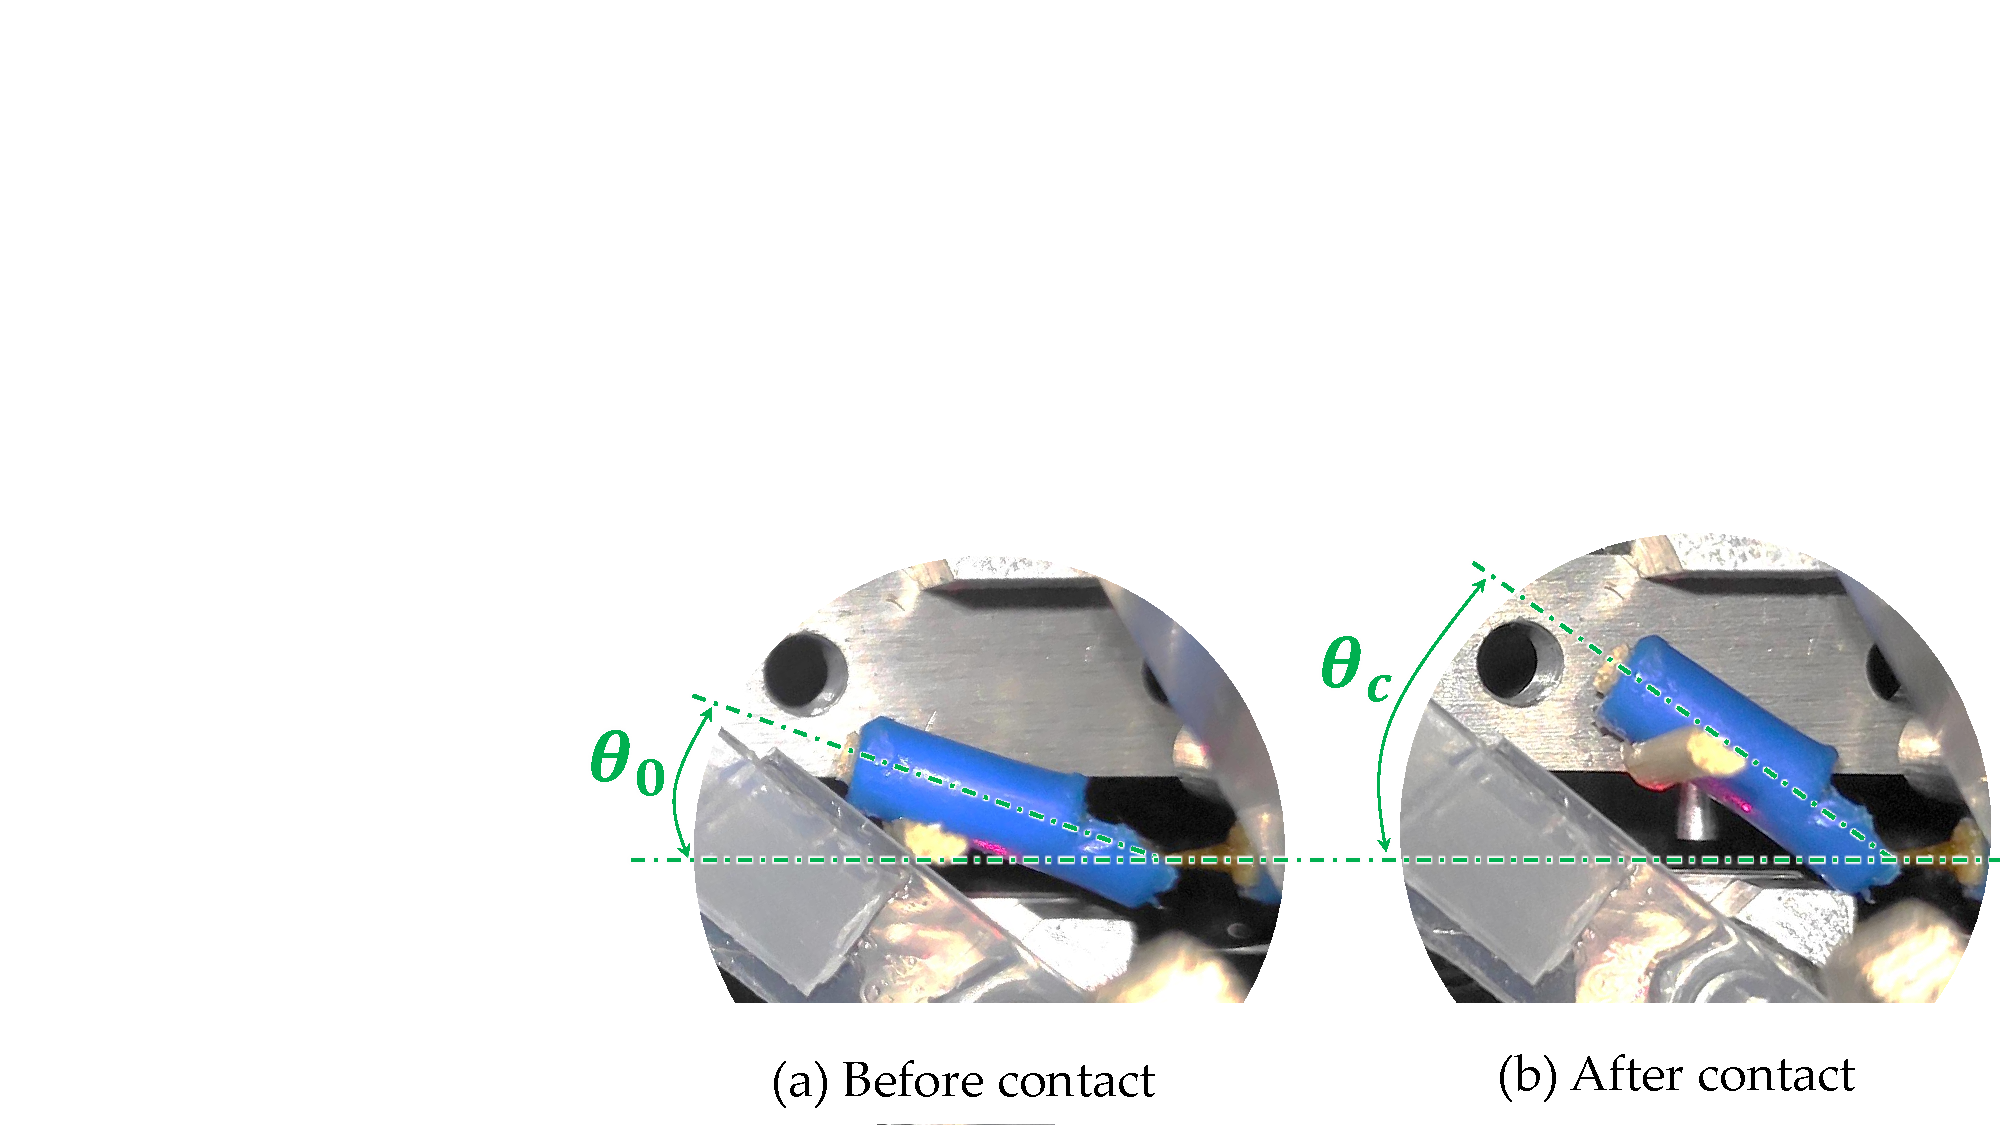
\includegraphics[trim={4cm 0cm 0cm 9.5cm},clip,width=0.7\textwidth]{figures/contact_M_VH_lachers.pdf}
	\caption{Image de la VH$_{T100p}$ lorsque $\theta_0$($x_m=-x_{0})$ et lorsque $\theta_f$($x_m=x_{0,vh}$)}
	\label{fig:contact_M_VH_lachers}
\end{center}
\end{figure}
%%%%%%%%%%%%%%%%%%%%%%%%%%%%%%%%%%%%

%%%%%%%%%%%%%%%%%%%%%%%%%%%%%%%%%%%
\begin{table}[!htbp]
	\centering
	% \resizebox{\textwidth}{!}{%
		\begin{tabular}[t]{c|c|c}
\toprule
\multicolumn{1}{c}{\textbf{Paramètre}}	&
\multicolumn{1}{c}{\textbf{Valeur OB}} 	& 
\multicolumn{1}{c}{\textbf{Valeur OBVH}}  \\
\midrule
$D_g$ [mm] 						& \cellcolor{ashgrey} 		& \textcolor{red}{4} 		\\ \hline
$\Delta\theta$ [deg] 			& \cellcolor{ashgrey} 		& \textcolor{red}{{[$\approx$ 19 ; $\approx$ 36]}} \\ \hline
$K_{T100p}(\theta_f)$ [Nmm/rad] & \cellcolor{ashgrey}  		&  0.27 					\\ \hline
$a$ [mm]         			    & \cellcolor{ashgrey}  		&  2.24				 	 	\\ \hline
$\mu_{fs}$ [~~] 				& \cellcolor{ashgrey}  		&  0.42  					\\ \hline
$K$ [N/m] 						&	84480			  	 	&  84480  					\\ \hline
$x_0$ [mm] 						& \textcolor{red}{0.59}		& \textcolor{red}{0.50}  	\\ \hline
$v_0$ [mm/s] 					& \textcolor{red}{10}		& \textcolor{red}{65}  		\\ \hline
$Q$	[~~] 						& 		24.0		 		& 5.0     					\\ \hline
$k^2_{sys}$ [\%] 				& 		1.25		 		& \textcolor{red}{1.25}   	\\ \hline
$\eta_{ob}$ [\%] 				& 		11.9		 		& 2.6   					\\ \hline	
$R_{ch}$ [k$\text{\ohm}$] 		&	\textcolor{red}{15.5}	& \textcolor{red}{15.5}    	\\ \hline		
$m$	[g]						    &	\textcolor{red}{5.88}	& 9.00   					\\ \hline	
$f_0$ [Hz]						&		32.9				& 27.9   					\\
\bottomrule	
	\end{tabular}
        \caption{Valeur des paramètres de l'OB et de l'ensemble OBVH implémentant le tube T100p suite au essais de lâchers expérimentaux}
        \label{tab:parametres lacher tube}
\end{table}        
%%%%%%%%%%%%%%%%%%%%%%%%%%%%%%%%%%%%

%/!\/!\/!\/!\/!\/!\/!\/!\/!\/!\/!\/!\/!\/!\/!\/!\/!\/!\/!\/!\/!\/!\/!\/!\%
\section{MODEL RECALIBRATION WITH EXPERIMENTAL DATA}
\label{sec:MODEL RECALIBRATION WITH EXPERIMENTAL DATA}
\section{ANALYZE AND DISCUSSION}
\label{sec:ANALYZE AND DISCUSSION}
%/!\/!\/!\/!\/!\/!\/!\/!\/!\/!\/!\/!\/!\/!\/!\/!\/!\/!\/!\/!\/!\/!\/!\/!\%

%/!\/!\/!\/!\/!\/!\/!\/!\/!\/!\/!\/!\/!\/!\/!\/!\/!\/!\/!\/!\/!\/!\/!\/!\%
\section{CONCLUSION}
\label{sec:CONCLUSION}
%/!\/!\/!\/!\/!\/!\/!\/!\/!\/!\/!\/!\/!\/!\/!\/!\/!\/!\/!\/!\/!\/!\/!\/!\%

%%%%%%%%%%%%%%%%%%%%%%%%%%%%%%%%%%%%%%
\begin{figure}[!htbp]
	\centering
	\captionsetup{justification=centering}
	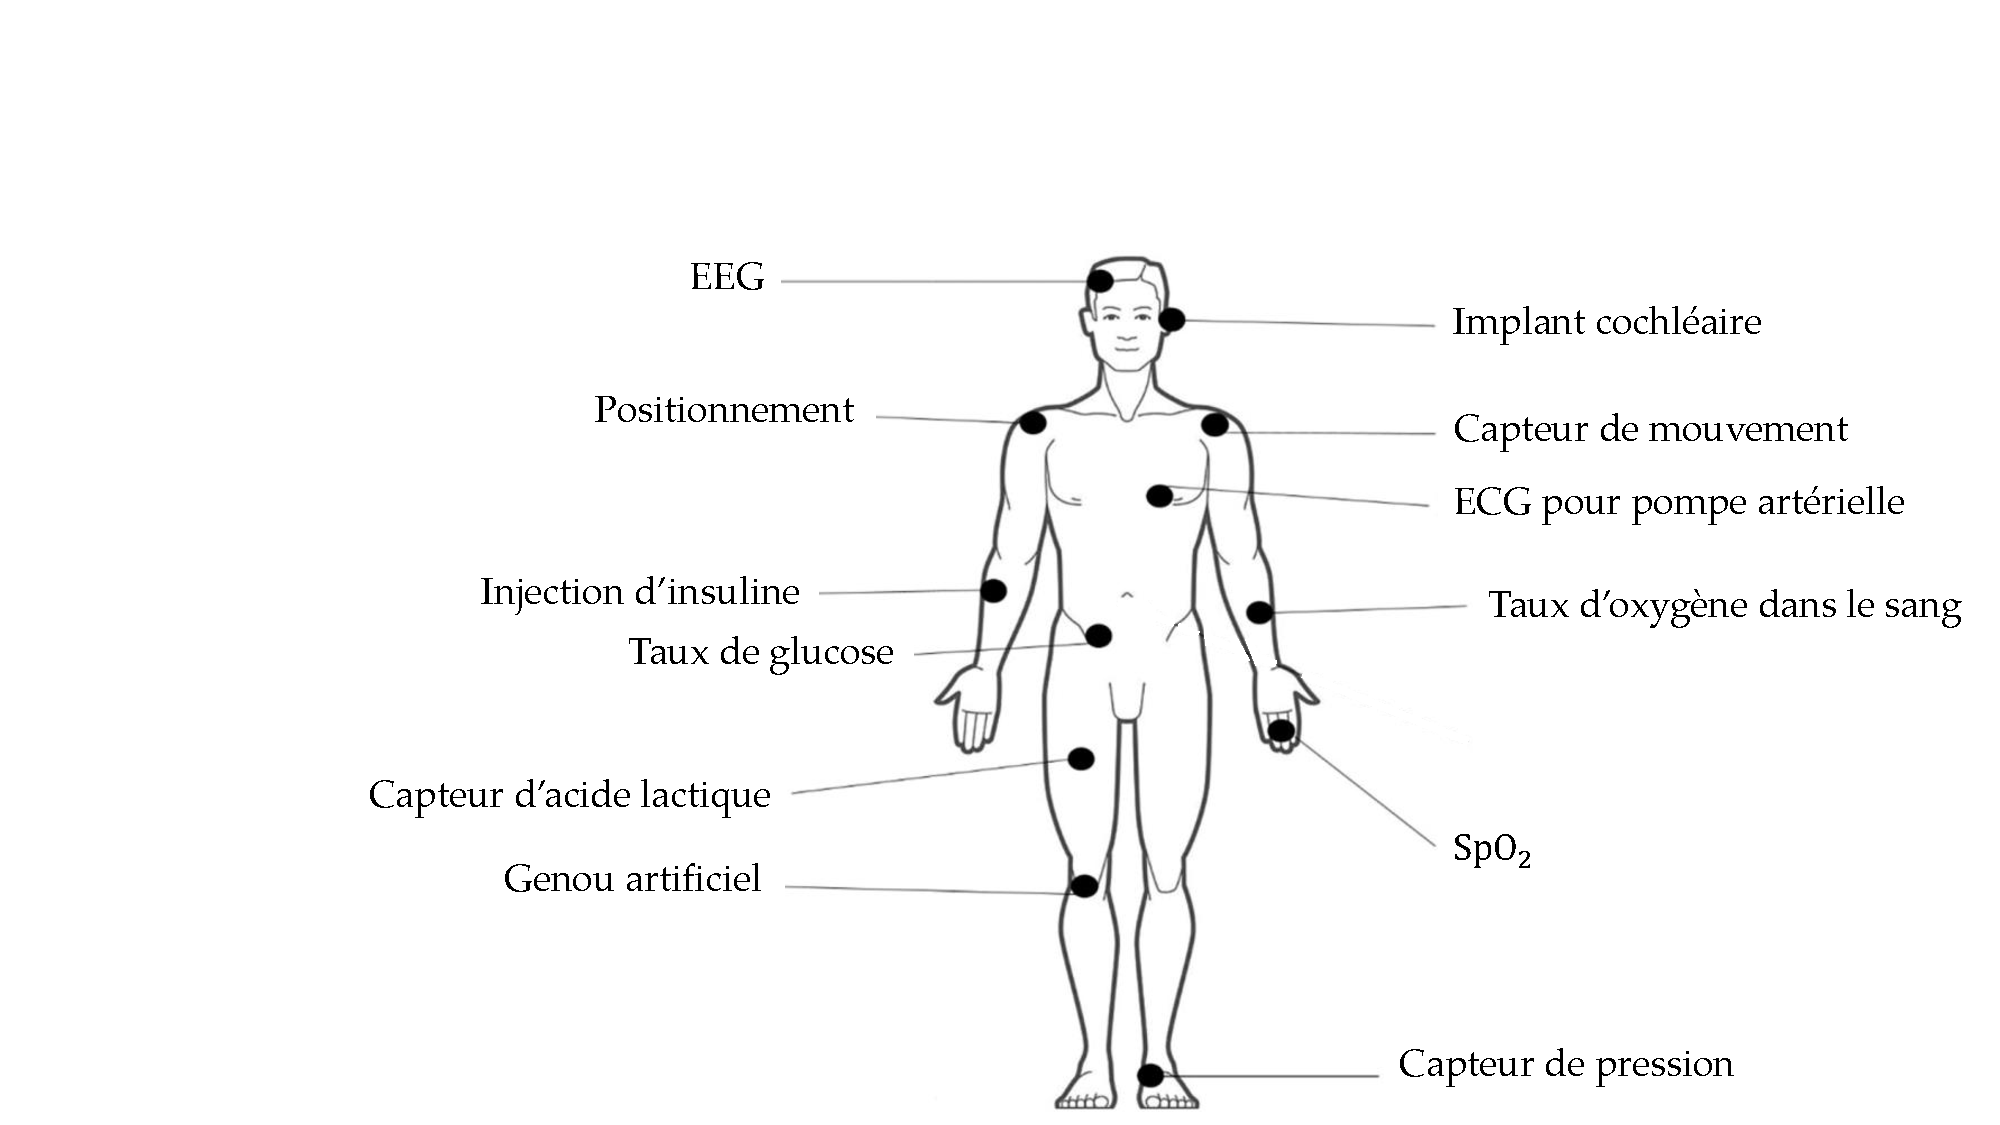
\includegraphics[trim={6cm 0cm 0cm 4cm},clip, width=0.5\textwidth]{figures/capteurs_corps_humain.pdf}
	\caption{Exemple de WBAN pour la télémédecine \cite{Abidi2020}.}
	\label{fig:capteurs_corps_humain}
\end{figure}
%%%%%%%%%%%%%%%%%%%%%%%%%%%%%%%%%%%%%%%


There is a worldwide growing interest on mobile devices in the region of the human head. Hearing aids, Bluetooth earphones, cochlear implants or wearables need to be supplied in energy for longtime use. As a complement to the batteries, or as a complete substitute, it is possible to provide this energy by harvesting it from the human head.\\
It is a common issue to see our mobile accessory off because it has no more battery. The high power density and the absence of moving parts make electrochemical energy storage the most practical and cheapest solution for portable powering \cite{Jiang2020}. However, over time, their autonomy decreases, and they also show instabilities when getting old, which can provoke leakage accidents resulting in chemical fires \cite{Tian2020}. Hence they need replacement, which can be difficult in many cases, as can be their recharging, and they also present a danger when used near human bodies. It is highly inconceivable that one day we could forgo the use of disposable batteries, but the energy harvesting can definitely complement their use by enhancing their autonomy, or in the best case substitute their use. 

Low power consumption hearing aids can operate with 1-2mW [Resound hearing aid datasheet].
Moreover, the cochlear implants can even be powered with a 150µW supply \cite{Cadei2014}. The issue is to exploit efficiently the thermal and mechanical energies produced by the human head and generally wasted in the air. The literature is filled of various studies trying to quantify the available energy and so numerous researchers have developed technologies capable to scavenge it.\\
The thermal energy is attractive because of the temperature stability of the human head. Some part of it is naturally evaporated by heat loss \cite{Starner1996}. Then, considering the Carnot efficiency and the figure of merit of the state of the art thermoelectric elements, the natural thermal radiation of human head makes available a power of 850µW to 2mW, depending on the ambient temperature \cite{Goll2011}. This amount is realistically reachable if the entire head is covered by thermoelectric wearables. Yet it is arduous to imagine an efficient wearable avoiding any discomfort if it has to fit all the available skin on the head. Thus the harvested power drops promptly by reducing the specific surface in contact witch the thermoelectric harvester.\\ 
The mechanical energy is much more exploited by the researchers because of the large panel of technological solutions compared to the thermoelectric transducers. \cite{Smilek2016} have been able to harvest 61 to 478µW from human walking phases, by placing resonating system on the head. Some others like \cite{Chaudhuri2017} went to the eardrum to scavenge its very low density vibration energy in order to supply energy for a cochlear implant.

The CRITIAS laboratory proved that the jaw movements create a dynamic motion in the ear-canal \cite{Carioli2016}. The latter is in fact compressed and bent when the temporomandibular joint comes in contact, as a consequence of the jaw motion. That periodic and natural phenomena generates a certain amount of energy that has been quantified. Carioli showed that the bending energy is in average 5 times higher than the compression energy, based on 12 subjects. However, as it is technologically difficult to adapt a transducer capable to harness the bending energy, they choose to concentrate on the ear canal compression energy which has a mean value of 2mW on the 12 test subjects. Their idea was to use an in-ear molding technology to produce personalized ear plugs capable to stick efficiently with the internal walls of the ear canal. Now there are two main issues for harvesting energy in the ear. The first one is to capture efficiently the compression energy and the second one is to convert it by minimizing the losses.\\
The developed electromagnetic harvester capable of harvesting 0.3µW in a single mastication cycle of 1.5Hz \cite{Delnavaz2012}. The poor efficiency can be explained by the scale reduction which is conversely proportional to the efficiency of electromagnetic conversion \cite{Arnold2007}. Their second harvester on the other hand uses a thin polyvinylidene fluoride (PVDF) film that envelopes the earplug to fit the ear canal walls \cite{Delnavaz2013}. The PVDF has been chosen for its great environmental compatibility and its flexibility. So the piezoelectric harvester has supplied 77µW per mastication cycle, a lot more than the electromagnetic transducer. Yet we need harder materials to improve the global efficiency but it could cause discomfort, or we need more place, which is limited by the ear canal. Further, the electromechanical coupling of piezoelectric polymers is known to be poor, and this parameter rules the electromechanical transducer’s capacity to harvest energy \cite{Roundy2005}.

The ear canal deflection energy is not a usual source because of the soft tissues and the low frequency of mastication. Thus the traditional transducing methods are not suitable enough for the application. Nevertheless, the frequency-up conversion could benefit to adapt the source to harvesters with better electromechanical coupling \cite{Ashraf2011}. Galchev et al. \cite{Galchev2009} used permanent magnets coupled to coils to rise the frequency of an ambient vibration source with a bistable mechanism. Kulah et al. \cite{Kulah2008} designed a complex but compact system with flat coils on cantilevers and permanent magnets to get a frequency-up conversion. A majority of the papers use as well mechanical stops with piezoelectric ceramic cantilevers to rich high frequencies with a good mechanical coupling \cite{Edwards2013,Gu2011,Lee2007}. Our application is not suitable for magnetic interactions because of the high non-linearities of magnetic fields at small scales. The piezoelectric ceramics yet appear like a good candidate, but the use of mechanical stops is very dissipative, and the contact shall wear the parts at long-term.\\
The paper is composed of \emph{X chapters}. The second chapter shows how the frequency-up conversion occurs through the bistable resonator under an external mechanical solicitation. The third chapter develops the design method we followed to couple the ear to the resonator through hydraulic circuits. This will bring us to the fourth chapter that establishes the hydraulic passive switches needed to cycle the bistable movement. Finally, the next chapters discuss the results and conclude the study.
%/!\/!\/!\/!\/!\/!\/!\/!\/!\/!\/!\/!\/!\/!\/!\/!\/!\/!\/!\/!\/!\/!\/!\/!\%
%/!\/!\/!\/!\/!\/!\/!\/!\/!\/!\/!\/!\/!\/!\/!\/!\/!\/!\/!\/!\/!\/!\/!\/!\%
%/!\/!\/!\/!\/!\/!\/!\/!\/!\/!\/!\/!\/!\/!\/!\/!\/!\/!\/!\/!\/!\/!\/!\/!\%

\newpage
\section{Frequency-up conversion}

% The \cref{fig:critias_harvesters} shows the 2 different transducing technologies that Delnavaz and al. used to exploit this energy. The electromagnetic harvester was actuated by a liquid filled earplug while the PVDF harvester fitted directly between the ear canal walls and the earplug.
% \begin{figure*}[!htbp]
% \begin{center}
% \captionsetup{justification=centering}
% \begin{subfigure} [h!]{0.49\textwidth}
% 	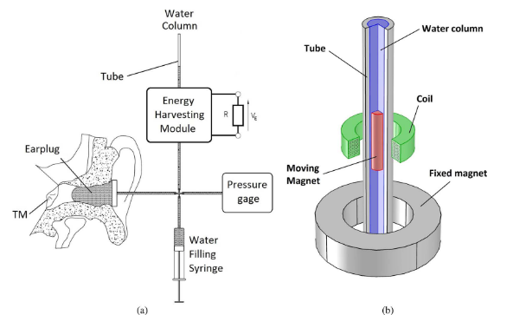
\includegraphics[width=\textwidth]{figures/critias_emag.png}
% 	\caption{Electromagnetic harvester \cite{Delnavaz2012}} \label{fig:critias_emag}
% \end{subfigure}
% %\hfill
% \begin{subfigure}[h!]{0.49\textwidth}
% 	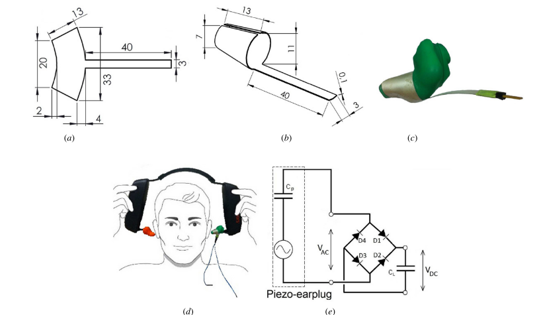
\includegraphics[width=\textwidth]{figures/critias_piezo.png}
% 	\caption{Piezoelectric harvester \cite{Delnavaz2013}}  \label{fig:critias_piezo}
% \end{subfigure}
% \caption{Micro harvesters developed by the CRITIAS laboratory}
% \end{center}
% \label{fig:critias_harvesters}
% \end{figure*}
For both those configurations, the energy source frequency was based on the mastication period. The previous studies show that the latter was about 1.5Hz. As mentioned in the previous chapter, the electromagnetic harvesters are not suitable for low frequency sources. Moreover, the low frequency actuation coupled to the PVDF very low electromechanical coupling coefficient lead to high energy losses and decrease so the global harvesting efficiency.
We use the liquid filled earplug as a pump defined by its pressure $p_e$ and its mass flow $q_e$, in order to externalize the harvesting device inside a hearing aid which is behind the ear. The amount of space allows the implementation of a frequency up converter which in our case is a bistable resonator.\\
The \cref{fig:mass_piston} shows a schematic view of the actuation of the harvester, by the ear deflection. The present structure is essentially composed of a liquid pressurized earplug, a bistable resonator containing lead zirconate titanate (PZT) structures and a hydraulic circuit allowing the coupling between those. Note that the bistable oscillator has two stable positions, called here $x_0$ and $-x_0$. The actuation occurs when the TM joint compresses the ear-canal walls, leading the fluid toward the piston. The latter pushes the resonator mass from its stable equilibrium position $x=x0$ until it is passed the potential barrier at its unstable equilibrium position ($x=0$). At this point the piston goes back due to the negative mass flow (\cref{fig:deltaV}) generated by the TM joint withdraw, while the mass goes resonate around the other stable equilibrium position at $x=-x_0$. The bistability of the resonator allows the frequency-up conversion of a quasi-static energy source, by maximizing the efficiency of the energy transfer and avoiding the use of wearing parts
\begin{figure}[!htbp]
\begin{center}
\captionsetup{justification=centering}
\begin{subfigure} [h!]{0.49\textwidth}
	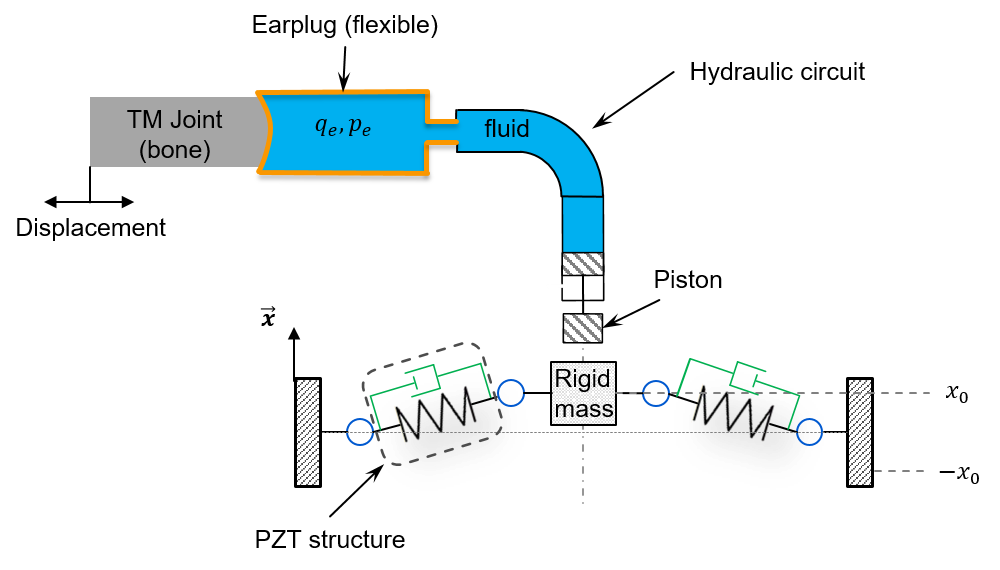
\includegraphics[width=\textwidth]{figures/masse_piston.png}
	\caption{Actuation for frequency-up conversion} \label{fig:deltaV}
\end{subfigure}
%\hfill
\begin{subfigure}[h!]{0.49\textwidth}
	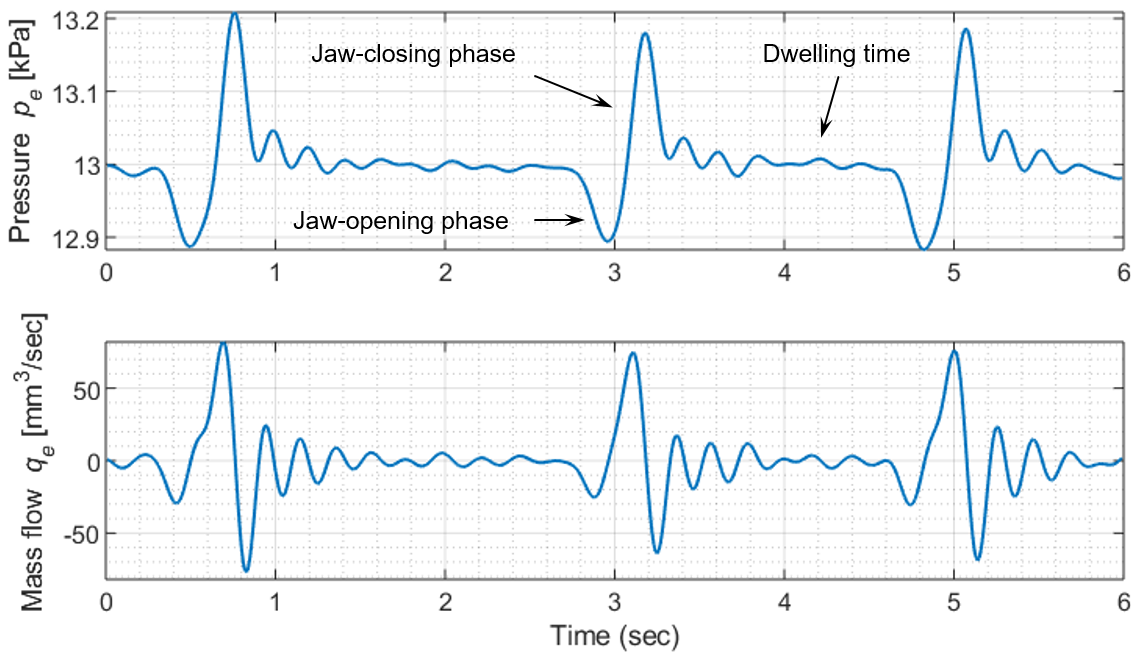
\includegraphics[width=\textwidth]{figures/deltaV.png}
	\caption{Earplug fluid pressure  and mass flow during mastication cycles}  \label{fig:mass_piston}
\end{subfigure}
\caption{Coupling between the energy source and the frequency-up converter}
\end{center}
\label{fig:frequency-up}
\end{figure}
\FloatBarrier
The \cref{fig:deltaV} shows the pressure
The bistable character of the resonator contributes to up the .






% The growing use of wireless devices and the miniaturization of electronic circuits have led to the development of Wireless Body Area Networks (WBAN) \cite{Latre2011}. These networks are composed of various sensors and actuators attached to clothing, or directly implanted on the human body. The diversity of devices and their wireless nature offer a new field of possibilities for innovative applications aimed at improving the health or life quality of users.\\










%% \appendix
%% \section{}
%% \label{}

%% If you have bibdatabase file and want bibtex to generate the
%% bibitems, please use
%%
%%  \bibliographystyle{elsarticle-num} 
%%  \bibliography{<your bibdatabase>}

%% else use the following coding to input the bibitems directly in the
%% TeX file.

%\begin{thebibliography}{00}
\bibliography{biblioArticle1.bib}
\bibliographystyle{elsarticle-num}
%\bibliographystyle{unsrt} 
%\end{thebibliography}


\end{document}
\endinput